\documentclass[12pt,a4paper,twoside,titlepage,openright,fleqn]{book}

\usepackage{thesis}

% User defined commands
% --------------------------
% --------------------------
% Macros and useful commands
% --------------------------
% --------------------------

% --------------------------
% Glossary
% --------------------------

\newcommand*\myglossaryentry[4]{
    % \index{#2@#1}
    \newglossaryentry{#2}{name={#1}, description={#3}, sort={#2}, #4}
}

\newcommand*\myacronym[2]{
    % \index{#1}
    \newacronym{#1}{#1}{#2}
}

% --------------------------
% Units
% --------------------------

\newcommand{\PeV}{{\rm \,PeV}}
\newcommand{\GeV}{{\rm \,GeV}}
\newcommand{\TeV}{{\rm \,TeV}}
\newcommand{\MeV}{{\rm \,MeV}}
\newcommand{\keV}{{\rm \,keV}}
\newcommand{\eV}{{\rm \,eV}}
\newcommand{\m}{{\rm \,m}}
\newcommand{\cm}{{\rm \,cm}}
\newcommand{\fm}{{\rm \,fm}}
\newcommand{\km}{{\rm \,km}}
\newcommand{\s}{{\rm \,s}}
\newcommand{\g}{{\rm \,g}}
\newcommand{\K}{{\rm \,K}}
\newcommand{\kyr}{{\rm \,kyr}}
\newcommand{\kyrs}{{\rm \,kyrs}}
\newcommand{\Myr}{{\rm \,Myr}}
\newcommand{\Myrs}{{\rm \,Myrs}}
\newcommand{\Gyr}{{\rm \,Gyr}}
\newcommand{\Gyrs}{{\rm \,Gyrs}}
\newcommand{\yr}{{\rm \,yr}}
\newcommand{\yrs}{{\rm \,yrs}}
\newcommand{\micron}{\,\mu\rm m}
\newcommand{\pc}{{\rm \,pc}}

% --------------------------
% Quantities
% --------------------------

\newcommand{\Msun}{M_\odot}
\newcommand{\Mstar}{M_\star}
\newcommand{\Rstar}{R_\star}
\newcommand{\vstar}{v_\star}
\newcommand{\vd}{v_d}
\newcommand{\tstar}{t_\star}
\newcommand{\Tstar}{T_\star}
\newcommand{\Tstareq}{T_{\rm eq}}
\newcommand{\Teff}{T_{\rm eff}}
\newcommand{\Lgam}{L_{\gamma}}

\newcommand{\muFn}{\mu_{F,n}}
\newcommand{\muFp}{\mu_{F,p}}
\newcommand{\muFe}{\mu_{F,e}}
\newcommand{\muFmu}{\mu_{F,\mu}}
\newcommand{\muFi}{\mu_{F,i}}
\newcommand{\qomax}{q_0^{\rm MAX}}
\newcommand{\qonorm}{q_0^{\rm norm}}
\newcommand{\qtr}{q^{\rm tr}}
\newcommand{\fMB}{f_{\rm MB}}
\newcommand{\fFD}{f_{\rm FD}}
\newcommand{\nFD}{n_{\rm FD}}
\newcommand{\Emax}{E_\chi^{\rm MAX}}
\newcommand{\sigmath}{\sigma_{\rm th}}
\newcommand{\sigmathi}{\sigma^{\rm th}_{i\chi}}
\newcommand{\kinFi}{\varepsilon_{F,i}}
\newcommand{\kinFn}{\varepsilon_{F,n}}
\newcommand{\tth}{t_{\rm therm}}
\newcommand{\tthn}[1]{\tth^{(n=#1)}}
\newcommand{\tthD}[1]{\tth^{(D#1)}}
\newcommand{\mbeff}{m_i^{\rm eff}}
\newcommand{\mneff}{m_n^{\rm eff}}
\newcommand{\mstar}{m_i^*}
\newcommand{\mcrit}{m_\chi^{\rm crit}}
\newcommand{\sigsurf}{\sigma_{\rm surf}}
\newcommand{\sigmav}{\langle \sigma_{\rm ann} v_\chi \rangle}

\newcommand{\erf}{{\rm \,Erf}}
\newcommand{\Msq}{|\overline{\mathcal M}|^2}


% --------------------------
% Editing
% --------------------------
\newcommand{\fixMV}[1]{\textbf{\textcolor{editcolor}{#1}}}

%%
%% VERSION HISTORY
%%    22 May 2006 - John Papandriopoulos - Original version
%%    12 Jul 2007 - John Papandriopoulos - Converted into template
%%    30 Sep 2015 - Maoyuan Liu - Draft version
%%    08 Aug 2020 - John Gargalionis - Draft version
%%    25 Sep 2023 - Michael Virgato - Draft version

% -----
% Basic
% -----

\usepackage{amsmath}
\usepackage{mathtools}
\usepackage{epsfig}
\usepackage{graphicx}
%Change to biblatex?
% \usepackage[numbers,sort&compress]{natbib}
\usepackage[backend=biber, style = numeric, url=false, isbn = false, sorting=none, citestyle=numeric-comp]{biblatex} 
% \addbibresource{references_zotero.bib}
\addbibresource{src/refs_main.bib}
\usepackage{color}
\usepackage{hyperref}

\usepackage{url}
\usepackage{enumitem}
% \usepackage{simplewick}
% \usepackage{simpler-wick}
\usepackage{pifont}
\newcommand{\cmark}{\text{\ding{51}}}
\newcommand{\xmark}{\text{\ding{55}}}
\usepackage{bm}

% For sans serif figure captions
% \usepackage[font=sf]{caption}
\usepackage{caption}
\usepackage{subcaption}
\usepackage{longtable}
\usepackage[version=3]{mhchem}

\usepackage{array}
\usepackage{makecell}
\newcolumntype{B}{>{\centering\arraybackslash}m{6cm}}
\newcolumntype{M}{>{\centering\arraybackslash}m{3cm}}
\newcolumntype{S}{>{\centering\arraybackslash}m{1.5cm}}

\usepackage{booktabs}
\usepackage{multirow}
\usepackage{colortbl}
\usepackage{tablefootnote}
\usepackage{csquotes} 
\usepackage{comment}

% math
\usepackage{slashed}



% Index
\usepackage{makeidx}
% \makeindex

% Glossary --> defitions of symbols and acronyms
\usepackage[toc,nonumberlist,nopostdot,abbreviations,automake]{glossaries-extra}
\usepackage{glossary-mcols}
\makeglossaries
\setglossarystyle{treegroup}

% ------
% Layout
% ------

% Suppress "This page intentionally left blank."
\newcommand*\markblankpages{}

% set page margins
%   these margins are set by the A4 paper ratios, 1:sqrt(2)
%   paperheight/paperwidth = paperwidth/textwidth = paperheight/textheight = sqrt(2)
%   outer/inner = bottom/top = sqrt(2)

%   Original version (top and bottom values for \symmetricmargin and \bookmargin
%   all the same)
  \usepackage[outer=36.02988mm,inner=25.47697mm,top=36.0317mm,bottom=50.9565mm]{geometry}
% \usepackage[outer=36.02988mm,inner=25.47697mm,top=21.8896mm,bottom=30.9565mm]{geometry}

%% For pdf copy
\newcommand*\symmetricmargin{
    \newgeometry{outer=30.7534mm,inner=30.7534mm,top=36.0317mm,bottom=50.9565mm}
  }

%% For book
\newcommand*\bookmargin{
  \newgeometry{outer=36.02988mm,inner=25.47697mm,top=36.0317mm,bottom=50.9565mm}
}

% For testing the formatting
\usepackage{lipsum}

\usepackage{tikz}
\usetikzlibrary{calc,decorations.markings, angles, quotes,backgrounds}
% \usepackage{tikz-feynman}

% ---------
% Eye candy
% ---------
\usepackage[
labelfont={small, bf, singlespacing},
textfont={small, singlespacing},
% justification={justified,RaggedRight},
singlelinecheck=false,
margin=0pt,
width=.9\textwidth,
figurewithin=chapter,
tablewithin=chapter]
{caption}
    
\usepackage[titletoc]{appendix}

% fancy chapter titles and quotes at beginning of title
\usepackage[beramono]{quotchap} 

\makeatletter
\renewcommand*{\sectfont}{\bfseries}
% \qsetcnfont{cm}
\renewcommand*{\chapnumfont}{%
  \usefont{T1}{\@defaultcnfont}{b}{n}\fontsize{100}{80}\selectfont% Default: 100/130
  \color{chaptergrey}%
}
\makeatother

% Draft watermark
\usepackage[contents={}]{background}
\usepackage[yyyymmdd,hhmmss]{datetime}

\newcommand*\DraftText{Draft compiled on \today\ at \currenttime}
\newcommand*\draft{
  \newcommand*{\archivalpapernote}{}
  \backgroundsetup{
    color=lightgray,
    position=current page.center,
    angle=90,
    vshift=0.45\paperwidth,
    opacity=1,
    scale=1,
    contents={\LARGE\ttfamily\DraftText}
  }
}

% -----
% My Colours
% -----

\definecolor{bluemv}{HTML}{2F76DC}
\definecolor{lightbluemv}{HTML}{62C3F8}
\definecolor{darkbluemv}{HTML}{003870}
\definecolor{lightbluemv}{HTML}{80DEEA}
\definecolor{magentamv}{HTML}{EC407A}
\definecolor{greenmv}{HTML}{5CA617}
\definecolor{darkredmv}{HTML}{FF1929}
\definecolor{redmv}{HTML}{f72a38}
\definecolor{orangemv}{HTML}{FF9239}
\definecolor{editcolor}{HTML}{e8be27}


\hypersetup{colorlinks, citecolor=bluemv, linkcolor=bluemv, urlcolor=bluemv, linktocpage=true}


% set draft watermark
% \draft

\newcommand{\Ncomm}[1]{{\footnotesize\color{red}\bf NB: #1}}

\begin{document}

%%
%% Frontmatter
%%
\begin{frontmatter}
  \frontmatterheadings
  % Dissertation title
\title{Dark Matter in Compact Objects (TBD)}

% Author
\author{Michael Virgato}

% Date of submission
\submissionmonth{XXX}
\submissionyear{XXX}

% Department
\department{School of Physics}

% University
% \university{\scshape The University of Melbourne}
\university{The University of Melbourne}

  % the title page is centered horizontally
  \symmetricmargin
  \maketitle
  %% Toggle this for pdf vs book
  % \bookmargin
  \begin{abstract}%
  DM in COs
  Heat up
  Maybe See
\end{abstract}

  \begin{publications}
 
  \begin{flushleft}
    Refs.~\cite{Bell:2020jou_sep_ImprovedTreatmentDark, Bell:2020lmm_mar_ImprovedTreatmentDark, , Bell:2020obw_sep_NucleonStructureStrong, Bell:2021fye_oct_Improvedtreatmentdark, Anzuini:2021lnv_nov_Improvedtreatmentdark, Bell:2023ysh_dec_ThermalizationAnnihilationDark} below are the journal publications, and preprints
    authored or co-authored during my PhD candidature. The authors are listed
    alphabetically in all of the titles.
  \end{flushleft}

  \journalpaperlist
  \begin{enumerate}[label={[\arabic*]}]
    \item Papers
  \end{enumerate}
\end{publications}

  \makedeclaration
  % \begin{contribution}
   I did $x$ and someone else did $y$.
\end{contribution}

  \begin{preface}


This thesis is comprised of seven chapters, with chapters~\ref{chapter:capture_intro} -~\ref{chapter:thermalisation} based on several of the papers produced during the completion of this degree, namely Refs.~\cite{Bell:2020jou_sep_ImprovedTreatmentDark, Bell:2020lmm_mar_ImprovedTreatmentDark, Bell:2021fye_oct_Improvedtreatmentdark, Anzuini:2021lnv_nov_Improvedtreatmentdark, Bell:2023ysh_dec_ThermalizationAnnihilationDark}. These papers can be thought of as a series of works, with the original motivation credited to Nicole Bell, Giorgio Busoni and Sandra Robles. Given that they build off each other, there is significant overlap between each paper so that they are each a self-contained piece of work.

The chapters of this thesis are written in a way that combines the ideas presented in these papers in a logical manner, with much of the overlapping content removed. 
The chapters of this thesis and my contributions to these works are as follows:
\begin{itemize}
    \item Chapter~\ref{chapter:introduction} forms an original introduction and review of the literature.
    \item Chapter~\ref{chapter:compactobjects} is an original introduction to compact objects. The discussion of the white dwarf equation of state and observational status is in large part taken from section 2 of Ref.~\cite{Bell:2021fye_oct_Improvedtreatmentdark} that was written by me.
    \item Chapter~\ref{chapter:capture_intro} begins with an original review of Gould's formalism for dark matter capture in the Sun. The remainder of the chapter combines results from Refs.~\cite{Bell:2020jou_sep_ImprovedTreatmentDark, Bell:2020lmm_mar_ImprovedTreatmentDark} to give a complete overview of the capture formalism developed in these papers. For Ref.~\cite{Bell:2020jou_sep_ImprovedTreatmentDark}, I made contributions to developing the code used in the numerical calculations, with version 1 of the code written by Giorgio Busoni, and to the analytic calculations for the interaction rates. I contributed to writing the sections discussing details of the formalism and the numerical results. In Ref.~\cite{Bell:2020lmm_mar_ImprovedTreatmentDark}, I made similar contributions to the writing and numerical calculations as the previous paper.
    \item The first half of Chapter~\ref{chapter:capture_leptons} discusses the main results for the capture of dark matter due to scattering on the leptonic species in neutron stars from Ref.~\cite{Bell:2020lmm_mar_ImprovedTreatmentDark}. The second half looks at dark matter interaction with electrons in white dwarfs in Ref.~\cite{Bell:2021fye_oct_Improvedtreatmentdark}. In this paper, the calculations and discussions involving dark matter-ion interactions are the work of Maura Ramirez-Quezada and are not included in this thesis. The calculations and text discussing the dark matter-electron interactions are my own work. In addition, I wrote the discussion and performed the numerical calculations of the white dwarf structure and equation of state.
    \item Chapter~\ref{chapter:capture_baryons} is based on the results of Ref~\cite{Anzuini:2021lnv_nov_Improvedtreatmentdark}. I contributed to the numerical calculations of $m^*$ (relevant for multiple scattering) and deep inelastic scattering. Much of the numerical code was reused from the previous papers. I also contributed to writing the sections discussing the interaction rates and the results of the capture rates and threshold cross-sections. 
    \item Chapter~\ref{chapter:thermalisation} is based on Ref.~\cite{Bell:2023ysh_dec_ThermalizationAnnihilationDark}. I performed all numerical calculations and wrote the first draft of the paper, save section 2, which was written by Sandra Robles. I contributed to the analytical approximations together with Giorgio Busoni.
    \item Chapter~\ref{chapter:conclusion} presents my concluding remarks on this thesis as a whole and the future directions of this work.
\end{itemize}
The plots presented in the published versions of the papers were all made by Sandra Robles. Only when necessary were these figures remade before being included in this thesis.
Any part of these papers I did not originally write was rewritten before being included in this thesis. 

The results of Ref.~\cite{Bell:2020obw_sep_NucleonStructureStrong} were not used in this thesis as I did not make significant contributions to the text.

Ref.~\cite{Bell:2024qmj_apr_HeavyDarkMatter} was written in large part by Sandra Robles and Giorgio Busoni and, as such, is not included in this thesis either. However, in this work, I performed the numerical calculations for the dark matter thermalisation times and wrote the first draft of that discussion.
\end{preface}

  \begin{acknowledgements}
  % General intro sentence
  % The completion of this thesis would not have been possible without all support 
  % Nicole

  First and foremost, thank you to my supervisor, Nicole Bell, for all the wisdom, guidance, and support you have provided me over the last five years. 

  % Collaborators
  I was fortunate enough to collaborate with Sandra Robles and Giorgio Busoni on many of the projects I worked on during my candidature. Thank you both for all that you have taught me over these years. In particular, I want to thank Sandra for always pushing me to do the best work possible. Your mentorship was truly appreciated.

  % Panel
  To the members of my advisory panel, Matthew Dolan and Andrew Melatos, thank you for all the guidance and encouragement you have provided over the years.

  % Office mates
  Returning to the office after nearly two years of COVID lockdowns solidified how important working alongside fellow students is to the PhD experience. In particular, I would like to thank Fred Hiskens, Maaz Hayat, Ayo Ore, Alex Ritter, Alexei Sopov, and Josh Wood for the countless hours of physics (and non-physics) related conversations we shared. You all made that office a truly wonderful place to work.
 
  % Friends
  I was lucky enough to meet and become good friends with many people in and around the physics department throughout my long tenure at this university. In particular, I would like to thank Marcel Hohmann, Mike Mews, Oliver Anagnostou, Daniel Marcantonio, Lachlan Milligan, and Neuton Li. Your friendship over these long years has been truly appreciated.

  % Parents and family
  Finally, I am incredibly thankful to my family for supporting me during this degree. Thank you for the love and encouragement you have provided over the years. 

  % Acknowledgement of country
  \vfill
  \noindent\rule{\textwidth}{0.5pt}
  \textit{I would like to acknowledge the traditional owners and custodians of the lands on which this work was completed, the Wurundjeri people of the Kulin nation, and pay my respects to Indigenous Elders past and present. Sovereignty has never been ceded. It is, was, and always will be, Aboriginal land.}
\end{acknowledgements}

  % \begin{dedication}
  No one.
\end{dedication}

  {\singlespacing
    \tableofcontents
    \clearpage
    \addcontentsline{toc}{chapter}{List of Figures}
    \listoffigures
    \clearpage
    \addcontentsline{toc}{chapter}{List of Tables}
    \listoftables
  }
\end{frontmatter}

%%
%% Main matter
%%
\begin{mainmatter}
  \mainmatterheadings
  \symmetricmargin
  %% General background
  \graphicspath{{img/chapter_1/}}

% \begin{savequote}
% ``Trying to reinvent the wheel is a lot of work. It's okay to make some tweaks and enjoy the ride." 
%     \qauthor{Karen Lamb}
% \end{savequote}

\chapter{Introduction}
\label{chapter:introduction}

% \begin{synopsis}
% Background on DM and its current status
% \end{synopsis}
%%%%%%%%%%%%%%%%%%%%%%%%%%%%%%%%%%%%%
%%%%%%%%%%%%%%%%%%%%%%%%%%%%%%%%%%%%%
%%%%%%%%%%%%%%%%%%%%%%%%%%%%%%%%%%%%%

Dark Matter is an enigma in modern physics. Despite the significant scientific
effort that has gone into trying to discern its nature, a definitive detection
proving its existence eludes us. Nevertheless, dark matter's influence 
on our Universe is undeniable, with evidence supporting its existence arising on \fixMV{all} scales, large and small.


%%%%%%%%%%%%%%%%%%%%%%%%%%%%%%%%%%%%%
%%%%%%%%%%%%%%%%%%%%%%%%%%%%%%%%%%%%%
%%%%%%%%%%%%%%%%%%%%%%%%%%%%%%%%%%%%%
\section{Evidence for Dark Matter}
%%%%%%%%%%%%%%%%%%%%%%%%%%%%%%%%%%%%%
%%%%%%%%%%%%%%%%%%%%%%%%%%%%%%%%%%%%%
%%%%%%%%%%%%%%%%%%%%%%%%%%%%%%%%%%%%%

Today, the amount of evidence in support of dark matter's existence is overwhelming. This evidence comes from astrophysical and cosmological observations inconsistent with a universe composed entirely of visible matter. This section serves as a review of this evidence. 

%%%%%%%%%%%%%%%%%%%%%%%%%%%%%%%%%%%%%
%%%%%%%%%%%%%%%%%%%%%%%%%%%%%%%%%%%%%
\subsection{Astrophysical Observations}
%%%%%%%%%%%%%%%%%%%%%%%%%%%%%%%%%%%%%
%%%%%%%%%%%%%%%%%%%%%%%%%%%%%%%%%%%%%

\subsubsection*{Galaxy Clusters}

Some of the first hints of dark matter's existence came from observations of galaxy clusters. Perhaps the most famous analysis was performed by Fritz Zwicky~\cite{Zwicky:1937zza_MassesNebulaeClusters}, who was puzzled by the high rotational velocities of galaxies within the Coma Cluster. By applying the virial theorem, equating the cluster's kinetic and gravitational potential energies, he found that the cluster would need to contain a much more significant amount of \textit{dunkle materie} (dark matter) than visible matter to accommodate these high velocities.

\subsubsection*{Rotation Curves of Spiral Galaxies}

The anomalous rotational velocities observed in galaxy clusters can also be observed at the galactic scale. The rotation curves of spiral galaxies, which relate the rotational velocities of stars to their distance from the galactic centre, were observed to be flat at large distances. From the observed distribution of visible matter, Newtonian mechanics predicts that the orbital velocity of a star a distance $r$ from the galactic centre, $v_\star(r)$, is related to the mass of the galaxy, $M(r)$, through
\begin{equation}
    v_\star(r) = \sqrt{\frac{G M(r)}{r}},
\end{equation}
indicating that the velocity should fall off as $1/\sqrt{r}$ at the outer regions of the galaxy where $M(r)$ is constant. Instead, observations of many spiral galaxies indicate that this velocity remains constant out to the galaxy's edge. 

A simple way to produce such a rotation curve is to introduce a spherically symmetric distribution of dark matter around the galaxy,
\begin{equation}
    \rho_{\mathrm{DM}}(r) = \frac{v_0^2}{4 \pi G r^2},
\end{equation}
that results in a constant rotational velocity of $v_0$ out to the galaxy edge. Detailed simulations of structure formation in a Cold Dark Matter (CDM) Universe indicate that the dark matter halo follows a Navaro-Frenk-White (NFW) profile, \fixMV{cite for NFW}
\begin{equation}
    \rho_{\mathrm{DM}}(r) = \frac{\rho_0}{\left( \frac{r}{r_\mathrm{s}}\right)\left( 1 + \frac{r}{r_\mathrm{s}}\right)^2},
\end{equation}
where $\rho_0$ and $r_\mathrm{s}$ are free parameters that must be fit to each halo. 
% More detailed simulations show that the true profile deviates slightly from an NFW, instead being more appropriately modelled by an Einasto profile. However, both profiles are observationally indistinguishable.

An example rotation curve for galaxy NGC 6503 is presented in Fig.~\ref{fig:gal_rotn_curve}, with the contributions from each of the matter components to the rotational velocity shown~\cite{Freese:2008cz_may_ReviewObservationalEvidence, Lelli:2016zqa_SPARCMassModels}. As can be seen, the visible matter constituting disk and gas components does not explain the observed rotational velocity. 

\begin{figure}[t!]
    \centering
    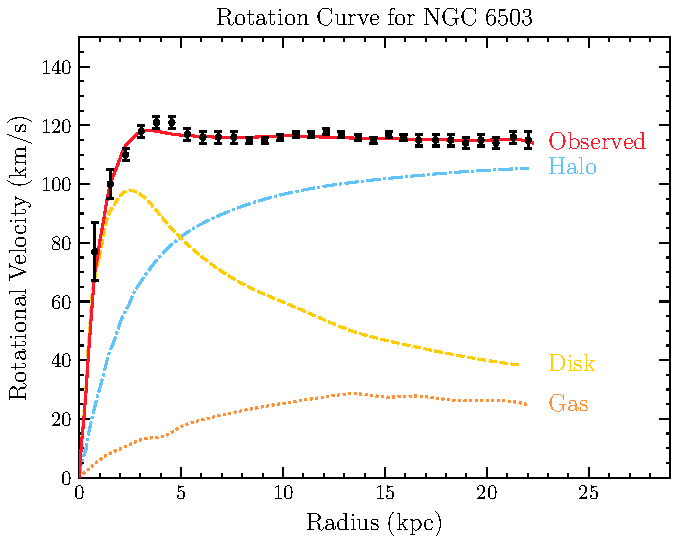
\includegraphics{gal_rotn_N6503}
    \caption{Galaxy rotation curve for NGC 6503, showing the contributions to the total velocity (red) from the DM halo (blue), disk (yellow), and gas components. Data used in making this plot was obtained from~\cite{Freese:2008cz_may_ReviewObservationalEvidence, Lelli:2016zqa_SPARCMassModels}.}
    \label{fig:gal_rotn_curve}
\end{figure}

\subsubsection*{Gravitational Lensing}

As General Relativity describes, the curvature of space-time around massive entities causes light to travel along curved paths. As such, the mass of astrophysical structures can be deduced from the extent to which objects in the background are gravitationally lensed. The disparity between the mass obtained from gravitational lensing and the mass of visible matter in the system is further evidence of dark matter's existence. 

\subsubsection*{The Bullet Cluster}

The bullet cluster is the result of two colliding galaxy clusters which the Chandra X-ray telescope imaged. When viewed in the X-ray, the smearing of the visible matter after the collision is clearly seen, as shown in the red regions of Fig.~\ref{fig:bullet_cluster}, which is expected from such a collision. However, when the gravitational potential was mapped using gravitational lensing, it was clear that the majority of the mass was displaced relative to the visible matter. This mass is attributed to the dark matter components of the original clusters. As indicated by the purple regions in Fig.~\ref{fig:bullet_cluster}, the dark matter halos seem to have passed through each other mostly unperturbed. This tells us that not only is the majority of the mass comprised of dark matter, but that the dark matter has extremely small interactions with both the visible matter and itself. 

\begin{figure}[t!]
    \centering
    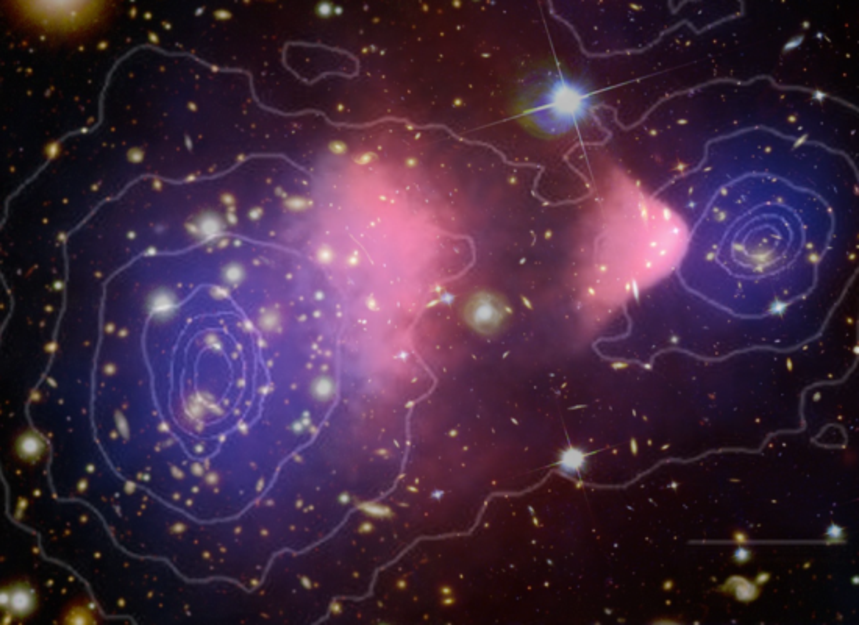
\includegraphics[width = 0.75\textwidth]{bullet_cluster}
    \caption{Image of the Bullet Cluster with contours of the gravitational potential superposed. The red regions indicate the baryonic matter after the collision, while the purple regions are the expected DM components deduced from gravitational lensing. \fixMV{cite}}
    \label{fig:bullet_cluster}
\end{figure}

%%%%%%%%%%%%%%%%%%%%%%%%%%%%%%%%%%%%%
%%%%%%%%%%%%%%%%%%%%%%%%%%%%%%%%%%%%%
\subsection{Cosmological Evidence}
%%%%%%%%%%%%%%%%%%%%%%%%%%%%%%%%%%%%%
%%%%%%%%%%%%%%%%%%%%%%%%%%%%%%%%%%%%%

Dark matter has played a major role in the cosmological history of our Universe. The current best cosmological model is the $\Lambda$-Cold Dark Matter model ($\Lambda$CDM), in which cold (i.e. non-relativistic) dark matter plays a prominent role. The relative amount of dark matter present in our Universe can be determined with measurements of the light element abundances produced via Big Bang Nucleosynthesis (BBN).

\subsubsection*{The Cosmic Microwave Background}
One of the best probes of cosmological models is the Cosmic Microwave Background (CMB). The CMB is the radiation that was emitted during recombination when the Universe had cooled enough for electrons and protons to combine and not be ionised by the photon bath. While the CMB temperature looks isotropic on large scales, fluctuations around the average value of $T_\mathrm{CMB} \sim 2.73\K$ are observed at very small scales. 
These anisotropies are the result of oscillations in the baryonic matter known as Baryon Acoustic Oscillations (BAO). These oscillations were produced due to the interplay between the outward pressure caused by matter interactions and the pull of gravitation due to dark matter. 

Measuring the angular power spectra of these anisotropies and fitting the cosmological parameters of the $\Lambda$CDM model tell us how the Universe's energy density ($\Omega_\mathrm{total}$), is partitioned between the matter ($\Omega_\mathrm{m}$), radiation  ($\Omega_\mathrm{rad}$), and dark energy  ($\Omega_\Lambda$) components. In a flat universe, of which we believe ours to be, these components should sum to $\Omega_\mathrm{tot} = 1$.
The Planck collaboration most recently performed a precise measurement of the CMB power spectrum in 2018, obtaining best-fit parameters
\begin{equation}
    \Omega_\mathrm{m} = 0.311 \pm 0.006,\quad \Omega_\Lambda = 0.689 \pm 0.006.
\end{equation}

Combining the predicted baryon density from BBN with the CMB observations breaks down the matter abundance into the dark ($\Omega_\mathrm{DM}$)  and baryonic ($\Omega_\mathrm{b}$) components yielding
\begin{equation}
    \Omega_\mathrm{DM}h^2 = 0.1193 \pm 0.0009,\quad \Omega_\mathrm{DM}h^2 = 0.02242 \pm 0.00014,
\end{equation}
where $h$ is the dimensionless Hubble constant such that the Hubble parameter today is $H_0 = 100\, h\km\s^{-1}\;\mathrm{Mpc}$. 

\subsubsection*{Large Scale Structure}
After recombination, the pressure on the baryonic matter from photons subsided, allowing the small density perturbations to grow. This would lead to the growth of stars, galaxies, and the large-scale structure we observe today~\cite{Springel:2006vs_LargescalestructureUniverse}. N-body simulations of the Universe's evolution require a cold dark matter component for this structure to form. While a small component of the dark matter can be warm, hot dark matter would wash out small-scale structures~\cite{Springel:2005nw_Simulatingjointevolution}.  

%%%%%%%%%%%%%%%%%%%%%%%%%%%%%%%%%%%%%
%%%%%%%%%%%%%%%%%%%%%%%%%%%%%%%%%%%%%
%%%%%%%%%%%%%%%%%%%%%%%%%%%%%%%%%%%%%
\section{Potential Models of Dark Matter}
%%%%%%%%%%%%%%%%%%%%%%%%%%%%%%%%%%%%%
%%%%%%%%%%%%%%%%%%%%%%%%%%%%%%%%%%%%%
%%%%%%%%%%%%%%%%%%%%%%%%%%%%%%%%%%%%%

The general consensus amongst physicists is that dark matter has a particle nature, similar to the visible matter of the Standard Model. Models may be as simple as dark matter being described by a single field or there could be an extensive hidden sector with complicated symmetry structures. Given the few details we know about dark matter, there exists an enormous library of models that can produce a viable dark matter candidate. However, there are generic properties a good dark matter candidate must satisfy, namely:
\begin{itemize}
    \item \textbf{Stable on Cosmological Timescales:} Dark matter must either be stable or have a lifetime significantly longer than the age of the Universe in order to be present in its current abundance. 
    
    \item \textbf{Neutral or milli-charged under Electromagnetism:} Dark matter, as its name suggests, does not significantly interact with light. By requiring that dark matter be completely decoupled from the Standard Model plasma by the time of recombination yields an upper bound on the milli-charge dark matter can carry of~\cite{McDermott:2010pa_TurningLightsHow} 
    \begin{equation}
        q_\mathrm{DM}/e < \begin{cases}
            3.5\times10^{-7} \left( \frac{m_\mathrm{DM}}{1\GeV}\right)^{0.58},\quad m_\mathrm{DM} > 1\GeV\\
            4.0\times 10^{-7}\left( \frac{m_\mathrm{DM}}{1\GeV}\right)^{0.35},\quad m_\mathrm{DM} <1\GeV,
        \end{cases}
    \end{equation}
    
    \item \textbf{Small Self-Interactions:} The standard $\Lambda$CDM cosmology assumes that the dark matter is collisionless. However, small dark matter self-interactions can help resolve existing small-scale structure issues~\cite{Tulin:2017ara_feb_DarkMatterSelfinteractions, Spergel:1999mh_Observationalevidenceselfinteracting}. Current limits on the self-interaction cross section are $\sigma_{\mathrm{DM-DM}}/m_\mathrm{DM} < 0.48\cm^2/\mathrm{g}$ come from merging galaxy clusters~\cite{Randall:2008ppe_ConstraintsSelfInteractionCrossSection} and the ellipticity of galaxies obtained from X-ray observations~\cite{Buote:2002wd_ChandraEvidenceFlattened}.
\end{itemize}
A selection of the more prominent dark matter candidates is shown in Fig.~\ref{fig:DM_models_landscape}. The key features of a few of these models are discussed below.

\begin{figure}[t!]
    \centering
    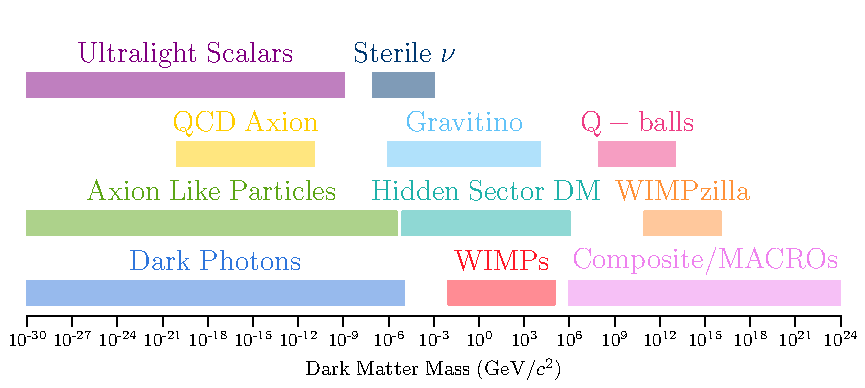
\includegraphics{DM_model_landscape}
    \caption{Illustrative landscape of dark matter models and the mass range for which they predict a valid candidate.}
    \label{fig:DM_models_landscape}
\end{figure}

\subsubsection*{WIMPs}
The Weakly Interacting Massive Particle (WIMP) is perhaps the most well-known dark matter candidate. WIMPs rose to fame thanks to the so-called ``WIMP miracle"~\cite{Feng:2010gw_DarkMatterCandidates}. This refers to the fact that particles with weak scale masses and annihilation cross sections just so happen to have the correct relic abundance of dark matter when produced via the freeze-out mechanism~\cite{Jungman:1995df_Supersymmetricdarkmatter}. In this scenario, the final WIMP abundance depends on the total annihilation cross-section, $\langle\sigma v\rangle$, with only a very mild dependence on the DM mass~\cite{Steigman:2012nb_PreciseRelicWIMP}, 
\begin{equation}
    \Omega_{\mathrm{DM}}h^2 \sim 0.12 \; \left(\frac{2.2\times 10^{-26}\cm^3 \s^{-1}}{\langle \sigma v\rangle}\right).
\end{equation}

The canonical weak-scale WIMP has been tightly constrained from direct and indirect detection limits, leading it to be disfavoured as a dark matter candidate. The term ``WIMP"  is now typically used to refer to any particle dark matter candidate that is produced thermally in the early Universe. Such a particle can have a mass in the range $10\MeV\lesssim m_\mathrm{WIMP} \gtrsim 100\TeV$. Lighter WIMPs will have non-negligible contributions to the effective number of neutrino species, $N_{eff}$, which is constrained through BBN and the Cosmic Microwave Background CMB to be $N_{eff} = 2.99 \pm 0.17$~\cite{Planck:2018vyg_sep_Planck2018results}. Masses larger than $\sim 100\TeV$ are excluded from partial wave unitarity~\cite{Griest:1989wd_UnitarityLimitsMass}. 

\subsubsection{Axions}

The original axion was proposed by Peccei and Quinn~\cite{Peccei:1977hh_CPConservationPresence} as part of a dynamical solution to the ``Strong CP Problem". This refers to the measured value of the neutron electric dipole moment (nEDM) being anomalously small, with a current upper bound of $|d_n| < 0.18\times 10^{-26}\;e\cm$~\cite{Abel:2020pzs_feb_MeasurementPermanentElectric}. This can be translated to an upper bound on the CP-violating QCD $\theta$-parameter such that $|\theta_{QCD}|\lesssim 10^{-10}$, raising questions as to why this value seems to be fine-tuned to such a small value. 

The Peccei-Quinn solution to this problem introduces a new, anomalous, global  $U(1)_{\mathrm{PQ}}$ symmetry and promotes $\theta_\mathrm{QCD}$ to be a dynamical field.
The axion emerges as the pseudo-Goldstone boson associated with the breaking of $U(1)_\mathrm{PQ}$, such is in the two most prominent UV completions of the axion, the KSVZ~\cite{Kim:1979if_WeakInteractionSinglet, Shifman:1979if_CanConfinementEnsure} and DFSZ~\cite{_PossibleSuppressionAxion, Dine:1981rt_SimpleSolutionStrong} models. In these models, the axion produced in the early Universe can serve the role of cold dark matter today. This makes it a very compelling dark matter candidate, as it solves two of the biggest mysteries of physics in one neat package. 

However, solving the Strong CP problem can be rather restrictive on the model parameters. For example, the QCD axion's coupling to the photon is not a free parameter and depends on the scale at which the PQ symmetry is broken. Many models introduce a light pseudoscalar particle that is not associated with a solution to the Strong CP problem but has a coupling to the photon that takes the same form as the QCD axion. Such pseudoscalars are known as ``Axion Like Particles" (ALPs) and can similarly make a good dark matter candidate.

\commMV{Add some more candidates}

%%%%%%%%%%%%%%%%%%%%%%%%%%%%%%%%%%%%%
%%%%%%%%%%%%%%%%%%%%%%%%%%%%%%%%%%%%%
\subsection{Dark Matter in an Effective Fields Theory Framework}
\label{subsec:DM_EFTs}
%%%%%%%%%%%%%%%%%%%%%%%%%%%%%%%%%%%%%
%%%%%%%%%%%%%%%%%%%%%%%%%%%%%%%%%%%%%

\subsection{Overview of Effective Field Theory}
Given the sheer quantity of potential dark matter models and candidates, a model-independent approach for analysing experimental results is often desired. An economic analysis method is to use an Effective Field Theory (EFT) to describe the dark matter-Standard Model interactions. Effective theories are prevalent in all of physics, e.g., describing light using ray optics vs Maxwell's equations or the orbits of planets using Newtonian gravity vs General relativity. The delineating factor in choosing a formalism is the scale (energy, length, etc.) we are interested in. 
\commMV{Add in the usual EFT diagram}
Experiments will only be sensitive to interactions that can occur below some energy scale, i.e. $13.6\TeV$ at the LHC or $~1\GeV$ in direct detection experiments; we are only interested in describing the interactions that occur below this scale.

One follows two main schools of thought when constructing an EFT. First, there is the \textit{top-down} approach. Here, you begin with a particular complete model in mind that consists of heavy and light fields. At energies below the production threshold of the heavy fields, these degrees of freedom can be ``integrated out" of the theory. This process leaves an effective theory for the interactions amongst the light fields. The interactions that would be mediated by the heavy fields appear as non-renormalisable operators that are suppressed by this high energy scale, $\Lambda$. 

The second method, known as the \textit{bottom-up} approach, is more agnostic to the high-energy physics that might be in play. In this method, one constructs all possible operators that obey the required symmetries of the theory up to a desired mass dimension. Operators of mass dimension greater than four are then suppressed by powers the required number of powers of the high energy cutoff scale, $\Lambda$. This cutoff scale indicates the energy at which the EFT begins to break down and should at least be larger than the masses of the fields in the EFT. The Lagrangian constructed in this manner is made out of a tower of operators, $\mathcal{O}_i^{(n)}$, forming
\begin{equation}
    \mathcal{L}_\mathrm{EFT} \supset \sum_{n>4}   \sum_{i = 1}^{j_n} \frac{C_i^{(n)}}{\Lambda^{n-4}}\mathcal{O}_i^{(n)},
\end{equation}
where we sum over all $j_n$ operators present at mass dimension $n$. The $C_i^{(n)}$ are called Wilson coefficients and are typically energy dependent.


In the context of dark matter, there are many EFTs describing the interaction at various energy scales. For example, dark matter scatting off nuclei in direct detection experiments is described by a non-relativistic EFT built out of the momentum transfer, relative velocity and spin operators of the dark matter and targets~\cite{Cirelli:2013ufw_oct_Toolsmodelindependentbounds, Fitzpatrick:2012ix_EffectiveFieldTheory}. At higher energy scales where relativistic effects become important, the EFT is instead constructed from relativistic fields, such as dark matter that may be produced in colliders.

Generally, an EFT will have fewer free parameters than the underlying UV theories, typically the dark matter mass and the high energy cutoff scale. This is in contrast with the dozens or so parameters often present in complete models. This allows for a simpler interpretation of experimental results as you will be fitting to a lower dimensional parameter space. 

\commMV{Move the next sections later?}
\subsection{Dimension 6 EFT Operators for Dirac Fermion Dark Matter}
This work's approach will focus on dimension 6 EFT operators that describe the interactions of Dirac fermion dark matter with standard model fermions. These operators will have a structure 
\begin{equation}
    \mathcal{L}_\mathrm{EFT}^{(6)} \sim \frac{1}{\Lambda^2}(\bar{\chi}\Gamma_\mathrm{DM} \chi)(\bar{f}\Gamma_{\mathrm{SM}}f),
\end{equation}
where the $\Gamma_i$ determines the Lorentz structure of the interaction by taking appropriate combinations from the set
\begin{equation}
    \Gamma_i\in \{1, i\gamma_5, \gamma^\mu, i\gamma^\mu \gamma^5, \sigma^{\mu\nu}, i \sigma^{\mu\nu}\gamma^5\}.
\end{equation}
For example, the case of $\Gamma_\chi = \Gamma_\mathrm{SM} = 1$ yields scalar currents for both the DM and SM fermions and would correspond to integrating out a heavy scalar mediator in the UV theory. There are 10 such operators at dimension six that form a linearly independent basis. These are given in Table~\ref{tab:opers_defn_full}, along with spin-averaged squared matrix element for dark matter scattering with a fermion. The coupling constants, $g_f$, are given in terms of the fermion Yukawa couplings, $y_f$, and the EFT cutoff scale, $\Lambda_f$. Hence, these operators describe interactions between dark matter and the elementary fermions of the Standard Model: the leptons and quarks. 




\begin{table}[t!]
\centering
\setlength{\tabcolsep}{0.25em}   
\begin{tabular}{  c  c  c  c  c }
\toprule
  Name & Operator & $g_f$  & $|\overline{M}(s,t,m_i)|^2$   \\\midrule\midrule
  D1 & $\bar\chi  \chi\;\bar f  f $ & $\frac{y_f}{\Lambda_f^2}$  & $ g_f^2\frac{\left(4 m_{\chi }^2-t\right) \left(4 m_{\chi }^2-\mu ^2   t\right)}{\mu ^2}$ \\  
  D2 & $\bar\chi \gamma^5 \chi\;\bar f f $ & $i\frac{y_f}{\Lambda_f^2}$ & $g_f^2\frac{t \left(\mu ^2 t-4 m_{\chi }^2\right)}{\mu ^2}$ \\  
  D3 & $\bar\chi \chi\;\bar f \gamma^5  f $&  $i\frac{y_f}{\Lambda_f^2}$  &  $g_f^2 t \left(t-4 m_{\chi }^2\right)$ \\ 
  D4 & $\bar\chi \gamma^5 \chi\; \bar f \gamma^5 f $ & $\frac{y_f}{\Lambda_f^2}$  & $g_f^2 t^2$  \\
  D5 & $\bar \chi \gamma_\mu \chi\; \bar f \gamma^\mu f$ & $\frac{1}{\Lambda_f^2}$ &  $2 g_f^2 \frac{2 \left(\mu ^2+1\right)^2 m_{\chi }^4-4 \left(\mu ^2+1\right) \mu ^2 s m_{\chi }^2+\mu ^4 \left(2 s^2+2 s t+t^2\right)}{\mu^4}$ \\ 
  D6 & $\bar\chi \gamma_\mu \gamma^5 \chi\; \bar  f \gamma^\mu f $ & $\frac{1}{\Lambda_f^2}$ & $2  g_f^2\frac{2 \left(\mu ^2-1\right)^2 m_{\chi }^4-4 \mu ^2 m_{\chi }^2 \left(\mu ^2 s+s+\mu ^2 t\right)+\mu ^4 \left(2 s^2+2 s   t+t^2\right)}{\mu^4}$ \\ 
  D7 & $\bar \chi \gamma_\mu  \chi\; \bar f \gamma^\mu\gamma^5  f$ & $\frac{1}{\Lambda_f^2}$ &  $2  g_f^2 \frac{2 \left(\mu ^2-1\right)^2 m_{\chi }^4-4 \mu ^2 m_{\chi }^2 \left(\mu ^2 s+s+t\right)+\mu ^4 \left(2 s^2+2 s t+t^2\right)}{\mu^4}$ \\  \
  D8 & $\bar \chi \gamma_\mu \gamma^5 \chi\; \bar f \gamma^\mu \gamma^5 f $ & $\frac{1}{\Lambda_f^2}$ & $2  g_f^2 \frac{2 \left(\mu ^4+10 \mu ^2+1\right) m_{\chi }^4-4 \left(\mu ^2+1\right) \mu ^2  m_{\chi }^2 (s+t)+\mu ^4 \left(2 s^2+2 s t+t^2\right)}{\mu ^4}$ \\  
  D9 & $\bar \chi \sigma_{\mu\nu} \chi\; \bar f \sigma^{\mu\nu} f $ & $\frac{1}{\Lambda_f^2}$ & $8  g_f^2 \frac{4 \left(\mu ^4+4 \mu ^2+1\right) m_{\chi }^4-2 \left(\mu ^2+1\right) \mu ^2 m_{\chi  }^2 (4 s+t)+\mu ^4 (2 s+t)^2}{\mu ^4}$ \\  
 D10 & $\bar \chi \sigma_{\mu\nu} \gamma^5\chi\; \bar f \sigma^{\mu\nu} f $ & $\frac{i}{\Lambda_f^2}$ &  $8  g_f^2\frac{4 \left(\mu ^2-1\right)^2 m_{\chi }^4-2 \left(\mu ^2+1\right) \mu ^2 m_{\chi }^2 (4 s+t)+\mu ^4 (2 s+t)^2}{\mu^4}$\\  \bottomrule
\end{tabular}
\caption{Dimension 6 EFT operators~\cite{Goodman:2010ku_ConstraintsDarkMatter} for the coupling of Dirac DM to fermions (column 2), together with the squared matrix elements DM-fermion scattering (column 5), where $s$ and $t$ are Mandelstam variables, $\mu=m_\chi/m_T$, and $m_T$ is the target mass. 
\label{tab:opers_defn_full} }
\end{table}

\subsection{Going from DM-Quark to DM-Nucleon Interactions}

The operators in Table~\ref{tab:opers_defn_full} describe dark matter interactions at the quark level, as these are the degrees of freedom most models are formulated with. However, we will primarily be interested in dark matter scattering with baryons, which requires taking the matrix element of the quark operators between baryon states, i.e. $\langle {\cal B} | \bar q \, \Gamma_q q| {\cal B}\rangle$. These matrix elements can be calculated through the application of Chiral Perturbation Theory (ChPT), giving a baryon level EFT. The operators of this EFT will have the same form as those in Table~\ref{tab:opers_defn_full}, with the obvious replacement of $f\rightarrow \cal B$, as well as additional form factors that take into account the structure of the baryons.

The required form factors for each operator have been calculated at zero momentum transfer in Ref.~\cite{Cirelli:2013ufw_oct_Toolsmodelindependentbounds} and are given by 
\begin{align}
c_{\cal B}^S(0) &= \frac{2 m_{\cal B}^2}{v^2}\left[\sum_{q=u,d,s}f_{T_q}^{(\cal B)}+\frac{2}{9}f_{T_G}^{(\cal B)}\right]^2,\\
c_{\cal B}^P(0) &= \frac{2 m_{\cal B}^2}{v^2}\left[\sum_{q=u,d,s}\left(1-3\frac{\overline{m}}{m_q}\right)\Delta_q^{(\cal B)}\right]^2,\\
c_{\cal B}^V(0) &= 9,\\
c_{\cal B}^A(0) &=  \left[\sum_{q=u,d,s}\Delta_q^{(\cal B)}\right]^2,\\
c_{\cal B}^T(0) &= \left[\sum_{q=u,d,s}\delta_q^{(\cal B)}\right]^2,
\end{align}
where  $v=246$ GeV is the vacuum expectation value of the SM Higgs field, $\cal B$ is the baryonic species,  $\overline{m}\equiv(1/m_u+1/m_d+1/m_s)^{-1}$ and $f_{T_q}^{(\cal B)}$, $f_{T_G}^{(\cal B)}=1-\sum_{q=u,d,s} f_{T_q}^{(\cal B)}$, $\Delta_q^{(\cal B)}$ and $\delta_q^{(\cal B)}$ are the hadronic matrix elements, determined either experimentally or by lattice QCD simulations\footnote{The superscript letters $S,\;P,\;V,\;A$ and $T$ stand for Scalar, Pseudoscalar, Vector, Axial-vector and Tensor interactions respectively. The corresponding operators are: D1-2 for $S$; D3-4 for $P$; D5-6 for $V$, D7-8 for $A$; and D9-10 for $T$.}. The specific values of these matrix elements for various baryons are provided in Appendix~\fixMV{ADD APPENDIX}.

These form factors are perfectly viable when considering interactions with momentum transfers $\lesssim 1\GeV$ such as in direct detection experiments. For energies greater than this, the internal structure of the baryon begins to be resolved, and an additional momentum-dependent form factor is required to account for this~\cite{_ElectromagneticStructureNucleon},
\begin{equation}
    F_{\cal B}(t) = \frac{1}{\left( 1 - t/Q_0\right)^2},
\end{equation}
where $t$ is the Mandelstam variable, and $Q_0$ is an energy scale that depends on the hadronic form factor. For simplicity, we will conservatively take $Q_0 = 1 \GeV$ for all operators.
Putting everything together, the squared coupling constants for dark matter-baryon interactions are obtained by making the replacement
\begin{equation}
    g_f^2 \rightarrow \frac{c^I_{\cal B}(t)}{\Lambda_q^4} \equiv \frac{1}{\Lambda_q^4}c_{\cal B}^I(0)F^2_{\cal B}(t),\quad I\in {S, P, V, A, T},
\end{equation}
in the matrix elements in the final column of Table~\ref{tab:opers_defn_full}.



%%%%%%%%%%%%%%%%%%%%%%%%%%%%%%%%%%%%%
%%%%%%%%%%%%%%%%%%%%%%%%%%%%%%%%%%%%%
%%%%%%%%%%%%%%%%%%%%%%%%%%%%%%%%%%%%%
\section{Current Status of Dark Matter Constraints}
%%%%%%%%%%%%%%%%%%%%%%%%%%%%%%%%%%%%%
%%%%%%%%%%%%%%%%%%%%%%%%%%%%%%%%%%%%%
%%%%%%%%%%%%%%%%%%%%%%%%%%%%%%%%%%%%%

In broad terms, there are three main ways that we can search for evidence of dark matter, often termed ``make it, shake it or break it". ``Make it" refers to dark matter being produced at colliders; ``break it" to searching for dark matter annihilation signals; and ``shake it" to direct detection of dark matter scattering. An illustrative way of depicting these processes is shown in Fig.~\fixMV{add usual diagram}. This section discusses the current status of these detection methods. 


%%%%%%%%%%%%%%%%%%%%%%%%%%%%%%%%%%%%%
%%%%%%%%%%%%%%%%%%%%%%%%%%%%%%%%%%%%%
\subsection{Collider Bounds}
%%%%%%%%%%%%%%%%%%%%%%%%%%%%%%%%%%%%%
%%%%%%%%%%%%%%%%%%%%%%%%%%%%%%%%%%%%%

If dark matter is produced in a collider, it will simply leave the 
detector without depositing any energy. 
In order to determine if such an invisible particle was produced, 
conservation of energy-momentum is used to determine if 
there are any events that are missing energy. In practice, what 
is searched for is missing momentum that is transverse to the beamline.

Currently, dark matter has not been observed to be produced in particle colliders. This non-observation has instead been used to constrain the dark matter mass and production cross sections or couplings of various models. 
These limits are typically interpreted in a model-dependent manner, as different dark matter - Standard model couplings can significantly alter the production rates.
As mentioned above, EFTs can be used to explore a variety of interactions in a somewhat model-independent way.
However, many applications of this nature did not hold up to scrutiny, as the EFTs were being applied at energies outside their regions of validity~\cite{Busoni:2013lha_jan_ValidityEffectiveField, Buchmueller:2013dya_EffectiveFieldTheory, Busoni:2014haa_ValidityEffectiveField, Busoni:2014sya_ValidityEffectiveField}, and so care is needed when applying such methods. 

 The ATLAS and CMS experiments at the LHC have performed analyses on various dark matter production mechanisms, including the exchange of a $Z/Z'$ or Higgs, EFTs and heavy mediators, and mono-jet searches~\cite{CMS:2017jdm_jul_Searchdarkmatter} \footnote{These searches refer to a single jet being produced alongside a pair of dark matter particles. This jet could be of Standard Model or dark sector origin, with the latter commonly referred to as ``mono-X" searches.}. Collider searches also offer complimentary probes of the dark matter-nucleon scattering cross-section~\cite{Ruppin:2014bra_oct_Complementaritydarkmatter}. 
 
 It is important to note that an observation of an invisible massive particle at a collider is not enough to infer that it is dark matter. Such an observation only tells us that such a particle exists but nothing about its abundance, meaning it could just be a sub-component of a larger dark sector. In order to identify whether or not this was a dark matter detection, complimentary observations from direct or indirect detectors would be required. 
 
%%%%%%%%%%%%%%%%%%%%%%%%%%%%%%%%%%%%%
%%%%%%%%%%%%%%%%%%%%%%%%%%%%%%%%%%%%%
\subsection{Direct Detection Searches}
%%%%%%%%%%%%%%%%%%%%%%%%%%%%%%%%%%%%%
%%%%%%%%%%%%%%%%%%%%%%%%%%%%%%%%%%%%%

Direct detection experiments vary wildly depending on the dark matter 
mass range they are trying to probe. For ALP dark matter that is wavelike, haloscope experiments 
such as ADMX~\cite{ADMX:2009iij_SQUIDbasedmicrowavecavity} and MADMAX~\cite{MADMAX:2019pub_mar_Newexperimentalapproach} 
attempt to convert ALPs to photons via the Primakoff effect. 
Searches for WIMP dark matter look for the dark matter scattering with some detector
material, causing it to recoil and release some energy. Given our focus on WIMP dark matter, 
this section will review the experimental status of these detectors.

The differential rate at which the incoming flux of dark matter will scatter
within a detector with $N_T$ targets, as a function of the recoil energy, $E_R$,
is given by
\begin{equation}
    \frac{d R(E_R, t)}{dE_R} = N_T \frac{\rho_\mathrm{DM}}{m_\mathrm{DM}}\int_{v>v_\mathrm{min}}^{v_\mathrm{esc}}v f(\Vec{v} + \vec{v}_E)\frac{d\sigma}{dE_R}\,d^3v,
\end{equation}
 and depends on the quantities:
\begin{itemize}
    % \item $\rho_\mathrm{DM}$ is the ambient dark matter density;
    % \item $m_\mathrm{DM}$ is the dark matter mass;
    \item $v_\mathrm{min}$ is the minimum dark matter velocity required by kinematics for a scattering event to occur;
    \item $v_\mathrm{esc} = 528\km\s^{-1}$ is the Milky Way escape velocity;
    \item $\vec{v}_E$ is the velocity of the Earth through the dark matter halo\footnote{This accounts for the orbit of the Earth around the Sun, which induces an annual modulation in the flux of DM.};
    \item $f(\vec{v} - \vec{v}_E)$ is the dark matter velocity distribution in the Earth's frame;
    \item $d\sigma/dE_R$ is the differential scattering cross-section.
\end{itemize}
Given the low interaction rate of dark matter, the expected event rate in 
detectors is very low, around one event per day, per kilogram of target material, per kiloelectronvolt deposited.
Having such a low event rate requires the detector to be situated in 
an extremely low background environment, such as underground laboratories. 

Direct detection experiments aim to probe two main types of dark matter interactions:
Spin-dependent (SD) and spin-independent (SI) scattering. SD interactions couple
to the overall spin of the target, while SI interactions are agnostic to this.
Therefore, experiments searching for SI interactions benefit from using nuclei with a large atomic number, $A$,
as the interaction cross-section will involve a coherent sum over all nucleons.
This leads to an $A^2$ enhancement of SI interactions compared to the SD counterpart.

\begin{figure}
    \centering
    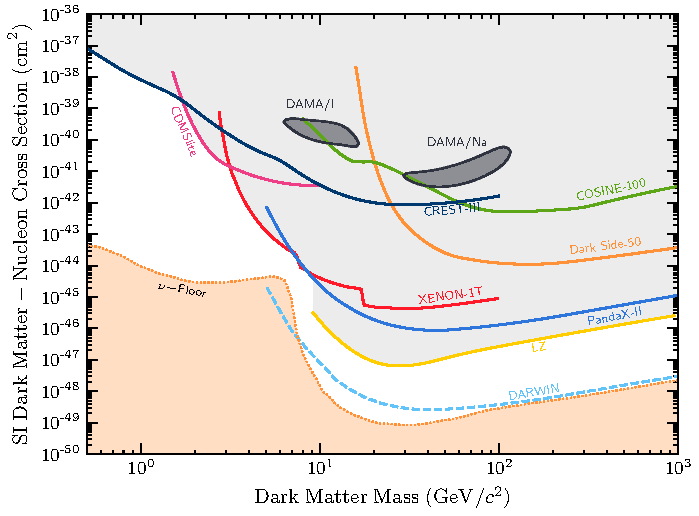
\includegraphics{img/chapter_1/DM_limits_SI.pdf}
    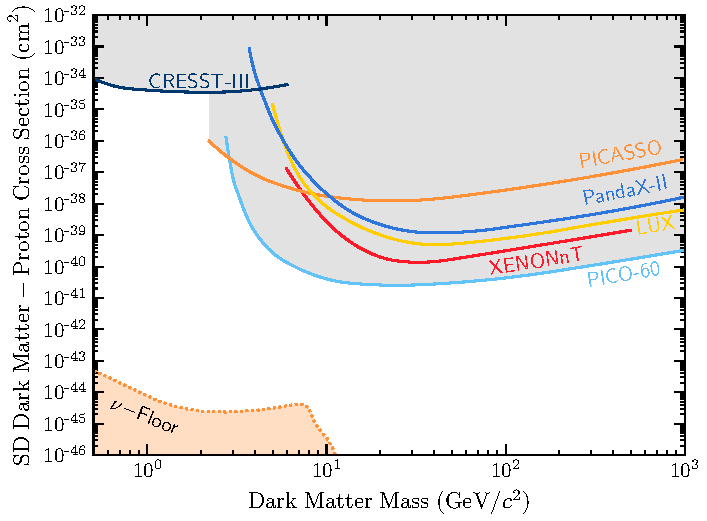
\includegraphics{img/chapter_1/DM_limits_SD_p.pdf}
    \caption{Current status of direct detection searches for dark matter. \textbf{Top:} Spin-independent dark matter-nucleon scattering. \textbf{Bottom:} Spin-dependent dark matter-proton scattering.}
    \label{fig:direct_detection_lims}
\end{figure}

The current leading constraints on the dark matter-nucleon scattering cross-section
are shown in Fig.~\ref{fig:direct_detection_lims}, with SI in the top panel and SD in the bottom.
The SI limits are set by liquid noble gas experiments (LZ~\cite{LZ:2022lsv_jul_FirstDarkMatter}, 
XENON-1T~\cite{XENON:2020gfr_mar_SearchCoherentElastic}, PandaX-II~\cite{PandaX-4T:2021bab_dec_DarkMatterSearch},
and DarkSide-50~\cite{DarkSide:2022dhx_mar_SearchDarkMatterNucleon}), solid-state cryogenic detectors (CRESST-III~\cite{CRESST:2019jnq_nov_FirstresultsCRESSTIII}, CDMSlite~\cite{SuperCDMS:2023sql_jun_SearchLowmassDark}, with projected DARWIN sensitivities~\cite{Aalbers:2022dzr_dec_Nextgenerationliquidxenon}), 
and room temperature crystals (DAMA/LIBRA~\cite{Savage:2008er_CompatibilityDAMALIBRA}, and COSINE-100~\cite{COSINE-100:2021xqn_nov_StrongconstraintsCOSINE100}). 

The SD experiments require their targets to carry non-zero spin for the dark matter to couple to. 
$\ce{^{19}F}$ is the favourable choice proton scattering, as it has an unpaired proton giving it its overall spin.
The leading constraints come from superheated liquid experiments such as the PICO-60~\cite{PICO:2019vsc_jul_Darkmattersearch} as well as PICASSO~\cite*{Behnke:2016lsk_apr_FinalResultsPICASSO}
In terms of the SD proton scattering shown in Fig~\ref{fig:direct_detection_lims},
These interactions are also searched for by many of the same experiments in the SI case, with the inclusion of
LZ's predecessor LUX~\cite{LUX:2017ree_jun_LimitsspindependentWIMPnucleon}.

The orange dashed line represents the neutrino floor\footnote{Calling this the ``neutrino fog" rather than floor has been gaining traction in recent years~\cite{OHare:2021utq_dec_Foghorizonnew}}, a theoretical lower limit on the discoverability of WIMP-like dark matter. In this region of parameter space, doctors will become sensitive to the irreducible background from neutrino scattering, which will produce signals almost indistinguishable from a true dark matter interaction. A significant amount of effort is being put toward overcoming this hindrance, with the main strategy being to take advantage of the directionality of dark matter flux~\cite{Grothaus:2014hja_jun_DirectionalDarkMatter}.

Many experiments begin to lose sensitivity to low-mass dark matter ($m_\mathrm{DM}\lesssim 10\GeV$) as the targets recoil with energies below the detector threshold. Current energy thresholds can reach as low as $\sim {\cal O} (100\eV)$, which is on the same order of magnitude as the recoil energy due to a $1\GeV$ dark matter collision. The sensitivity also falls off at a slower rate at larger masses, though this is due to the number of dark matter particles that pass through the detector given $N_\mathrm{DM} = \rho_\mathrm{DM}/m_\mathrm{DM}$, and the dark matter density is known to be $0.4\GeV \cm^{-3}$.

Direct detection limits also assume that the scattering cross-section is independent of the dark matter velocity and momentum transfer in the interaction. Given that the local dark matter dispersion velocity is predicted to be $v_d = 270\km\s^{-1} \approx 10^{-3}c$, a back-of-the-envelope estimation for the momentum transfer gives $q_\mathrm{tr}\lesssim 100 \MeV$. Therefore, cross-sections proportional to $v_\mathrm{DM}$ or $q_\mathrm{tr}$ will result in significantly lower event rates and hence much weaker limits than the unsuppressed interactions. 

This leads us to indirect detection methods, which can provide complementary probes to direct detection while also exploring interactions that are difficult, if not impossible, for terrestrial-based detectors to observe.
%%%%%%%%%%%%%%%%%%%%%%%%%%%%%%%%%%%%%
%%%%%%%%%%%%%%%%%%%%%%%%%%%%%%%%%%%%%
\subsection{Indirect Detection}
%%%%%%%%%%%%%%%%%%%%%%%%%%%%%%%%%%%%%
%%%%%%%%%%%%%%%%%%%%%%%%%%%%%%%%%%%%%

Indirect detection experiments aim to infer the presence of dark matter through its annihilation or decay into Standard Model states. 
These searches look for anomalies in astrophysical data, though dark matter accumulating within the Earth's core can also produce a detectable signal~\cite{Lee:2013iua_jan_Constrainingdarkmatter,ANTARES:2016bxz_jun_SearchDarkMatter}. The signals searched for include: 
\begin{itemize}
    \item Gamma-rays at terrestrial-based telescopes such as HESS~\cite{HESS:2018cbt_may_SearchgRayLine, Montanari:2023bzn_jul_Searchdarkmatter, HESS:2006zwn_ObservationsGalacticCenter}, VERITAS~\cite{VERITAS:2017tif_apr_DarkMatterConstraints, Ryan:2023yzu_jul_SearchDarkMatter, McGrath:2023oto_jul_IndirectsearchDark, Ryan:2023yzu_jul_SearchDarkMatter}, MAGIC~\cite{MAGIC:2009tyk_MAGICGammaRayTelescope, MAGIC:2011nta_SearchesDarkMatter, MAGIC:2011nta_SearchesDarkMatter, MAGIC:2009tyk_MAGICGammaRayTelescope} and HAWC~\cite{HAWC:2017mfa_feb_DarkMatterLimits, HAWC:2017udy_feb_SearchDarkMatter, HAWC:2017udy_feb_SearchDarkMatter, HAWC:2017mfa_feb_DarkMatterLimits, Proper:2015xya_jul_FirstLimitsDark, Harding:2015bua_jul_DarkMatterAnnihilation} as well as the Fermi-LAT~\cite{Fermi-LAT:2015att_nov_SearchingDarkMatter,Fermi-LAT:2015kyq_jun_UpdatedSearchSpectral,Fermi-LAT:2012ugx_FermiLATSearch, Fermi-LAT:2010qeq_ConstraintsCosmologicalDark, Su:2010qj_GiantGammarayBubbles} satellite;

    \item Neutrino signals at IceCube~\cite{IceCube:2016dgk_mar_Searchannihilatingdark, IceCube:2012ugg_mar_Searchdarkmatter}, ANTARES~\cite{ANTARES:2016bxz_jun_SearchDarkMatter,ANTARES:2016obx_may_SearchSecludedDark,ANTARES:2016xuh_aug_LimitsDarkMatter}, Super-K~\cite{Super-Kamiokande:2015xms_apr_Searchneutrinosannihilation,Super-Kamiokande:2004pou_Searchdarkmatter,Feng:2008qn_TestingDarkMatter}, and will be searched for at the upcoming Hyper-K~\cite{Bell:2020rkw_sep_SearchingSubGeVDark,Bell:2021esh_nov_Searchingdarkmatter,Bell:2022ycf_nov_Darkmatterpollution}, JUNO~\cite{Franarin:2018gfk_jun_JUNOSensitivityResonant} experiments.

    \item Cosmic-Rays by the AMS-02 experiment~\cite{Giesen:2015ufa_sep_AMS02antiprotonslast, Bergstrom:2013jra_oct_NewLimitsDark}
\end{itemize}

Signals from dark matter annihilation are best searched for by looking at regions where the dark matter density is expected to be high, boosting the annihilation rate. 
Natural places to look include the Galactic Centre~\cite{Ipek:2014gua_sep_RenormalizableModelGalactic,Fermi-LAT:2017opo_may_FermiGalacticCenter}, dwarf-spheroidal galaxies~\cite{Bonnivard:2015xpq_oct_Darkmatterannihilation}, and celestial bodies where dark matter can accumulate over time.
This last option is of primary interest to this work.

Stars have long been used to study various models of dark matter. 
ALPs of dark photons can be produced within the plasma of stars, altering the energy transport properties within them.
This can ultimately lead to deviations in the evolution of the star, which can be used to place some of the strongest constraints on these models~\cite{An:2013yfc_oct_Newstellarconstraints, Dolan:2022kul_oct_Advancingglobularcluster,Dolan:2023cjs_jun_ConstrainingDarkPhotons, }.
WIMP-like dark matter from the halo that couples to visible matter can scatter within the objects. 
The dark matter may lose enough energy in these interactions to become gravitationally bound to the object, leading to a population of dark matter being accumulated over time~\cite{Press:1985ug_Capturesungalactic, Gould:1987ju_WeaklyInteractingMassive, Gould:1987ir_ResonantEnhancementsWIMP,Jungman:1995df_Supersymmetricdarkmatter,Busoni:2017mhe_oct_Evaporationscatteringmomentum}. 

The capture of dark matter within the Sun has been extensively studied. The formalism set up by Gould~\cite{Gould:1987ir_ResonantEnhancementsWIMP,Gould:1987ju_WeaklyInteractingMassive,Gould:1991va_Bigbangarcheology} has remained quite successful, with many authors building on these foundations over time~\cite{Busoni:2017mhe_oct_Evaporationscatteringmomentum,Garani:2017jcj_may_DarkmatterSun,Bramante:2017xlb_sep_Multiscatterstellarcapture}
The captured dark matter can thermalise within the Sun's core, where it may annihilate and produce an observational signal. 
This could be via direct annihilation to neutrinos~\cite{Super-Kamiokande:2011wjy_IndirectSearchWIMPs,Super-Kamiokande:2015xms_apr_Searchneutrinosannihilation,ANTARES:2016obx_may_SearchSecludedDark,ANTARES:2016xuh_aug_LimitsDarkMatter,IceCube:2016dgk_Searchannihilatingdark}, or to some other long-lived state that can escape the Sun and decay into visible states~\cite{Batell:2009zp_SolarGammaRays,Schuster:2009au_TerrestrialSolarLimits,Bell:2011sn_Enhancedneutrinosignals,Feng:2016ijc_jun_DarkSunshineDetecting,Leane:2017vag_jun_PowerfulSolarSignatures}.
Additionally, WIMPs can also alter the energy transport within the Sun~\cite{Gould:1989hm_THERMALCONDUCTIONMASSIVE,Gould:1989ez_CosmionEnergyTransfer,Vincent:2013lua_apr_Thermalconductiondark,Geytenbeek:2016nfg_mar_Effectelectromagneticdipole}.

In comparison to DD searches, interpretation of indirect detection data will require additional model-dependent assumptions, namely the relevant annihilation channels of the dark matter. 
The most general limits can be placed by assuming that the dark matter only has a single annihilation channel, i.e. it annihilates to a $\tau^+\tau^-$ final state 100\% of the time. 
Under these assumptions, limits on the SD dark matter-proton cross-section have been placed that exceed current DD constraints, due to the rather large abundance of Hydrogen within the Sun. Constraints from the IceCube collaboration are shown in Fig.~\ref{fig:IceCube_2016_SD}

\begin{figure}[!t]
    \centering
    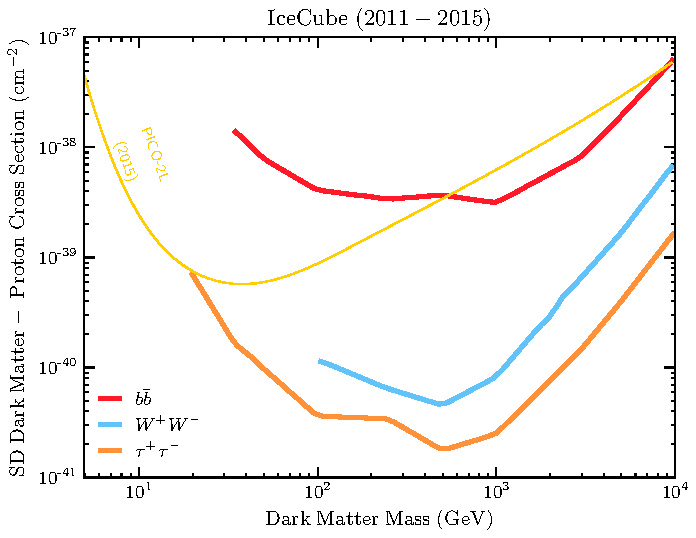
\includegraphics{IceCube_2016.pdf}
    \caption{Limits on the SD dark matter-proton cross-section from the IceCube collaboration assuming 100\% branching fraction to $b\bar{b}$ (red), $W^+ W^-$ (blue) or $\tau^+ \tau^-$ (orange) final states. Also shown is the result from the PICO-2L DD experiment. This plot was recreated with data taken from Ref.~\cite{IceCube:2016dgk_mar_Searchannihilatingdark}.}
    \label{fig:IceCube_2016_SD}
\end{figure}

The smallest dark matter mass that can be probed using solar capture is determined by the evaporation mass of the Sun. Below this mass, the dark matter will be efficiently evaporated out of the Sun at the same rate it is captured, thus no annihilation can take place~\footnote{A more rigorous definition of evaporation and evaporation mass will be presented later in the thesis.}.
Additionally, as with direct detection, the Sun will be far less sensitive to interactions that are proportional to the velocity/momentum transfer. 

Overcoming the first issue requires either a colder star or one that is much heavier. The second requires dark matter to scatter with the constituent material at relativistic energies to overcome the suppression in the cross-sections. 
Fortunately, there exists objects that meet all these criteria, allowing for a wider variety of dark matter models to be explored then direct detection or traditional indirect detection experiments: compact objects.

%%%%%%%%%%%%%%%%%%%%%%%%%%%%%%%%%%%%%
%%%%%%%%%%%%%%%%%%%%%%%%%%%%%%%%%%%%%
%%%%%%%%%%%%%%%%%%%%%%%%%%%%%%%%%%%%%
\section{Compact Objects as Dark Matter Probes}
%%%%%%%%%%%%%%%%%%%%%%%%%%%%%%%%%%%%%
%%%%%%%%%%%%%%%%%%%%%%%%%%%%%%%%%%%%%
%%%%%%%%%%%%%%%%%%%%%%%%%%%%%%%%%%%%%

The main goal behind this work is to explore how compact objects can be used to probe a wide variety of dark matter interactions that terrestrial direct detection experiments are insensitive to. By compact objects, we are referring to Neutron Stars (NSs) and White Dwarfs (WDs), and not Black Holes that also fall into this category.


Compact objects offer a unique laboratory for studying dark matter and its interactions with the Standard Model in environments unachievable anywhere else in the Universe. They generate strong gravitational fields and are composed of incredibly dense matter, with NSs reaching super-nuclear densities in their central cores. The capture rate within these objects is therefore enhanced due to these properties, with benefits over solar capture including:


\begin{itemize}
\item \textbf{Gravitational focusing of the DM flux:} The strong gravitational field will increase the impact parameter of the infalling dark matter. This increases the effective size of the capturing body, increasing the flux of dark matter passing through it. 

\item \textbf{Realtivistic Interaction Energies:} In general, the infalling dark matter will be accelerated to (semi-)relativistic velocities ($\sim 0.2 - 0.7 c$). Moreover, the stellar constituents will also have relativistic energies. As such, interactions that are momentum/velocity dependent will suffer far less suppression than in DD experiments. 

\item \textbf{Large Number of Targets:} The extremely high densities of these objects correspond to a considerable number of targets for scattering to occur. This allows these objects to probe very small scattering cross-sections, with NSs in particular expected to reach as low as $\sim 10^ {-45}\cm^2$. 

\item \textbf{\fixMV{Forgot the last point....}}
\end{itemize}

In the past, capture in NSs has been applied primarily in the context of sending gravitational collapse into black holes~\cite{McDermott:2011jp_ConstraintsScalarAsymmetric,Kouvaris:2011fi_ExcludingLightAsymmetric,Guver:2012ba_may_Capturedarkmatter, Garani:2018kkd_may_NewAnalysisNeutron,Bramante:2013nma_jan_Boundsselfinteractingfermion,Bertoni:2013bsa_dec_DarkMatterThermalization,Bell:2013xk_jun_Realisticneutronstar}, and the modifications of NS merger rates as well as the gravitational wave signatures of these mergers~\cite{Bramante:2017ulk_mar_SearchingDarkMatter, Ellis:2017jgp_jun_SearchDarkMatter, Ellis:2018bkr_jun_DarkMatterEffects,Nelson:2018xtr_jul_Darkhalosneutron}. Capture in WDs has also been considered, with a variety of different applications of the capture process~\cite{Steigerwald:2019efv_dec_DarkMatterThermonuclear, Panotopoulos:2020kuo_jun_Constraintslightdark, McCullough:2010ai_CaptureInelasticDark, Hooper:2010es_InelasticDarkMatter, Bramante:2015cua_sep_Darkmatterignition, Bertone:2007ae_CompactStarsDark}. 

In recent years, dark matter induced heating of NSs has reemerged as a potential detection frontier~\cite{Raj:2017wrv_feb_Neutronstarsdark, Baryakhtar:2017dbj_sep_DarkKineticHeating, Bell:2018pkk_sep_HeatingNeutronStars,Joglekar:2019vzy_sep_Relativisticcapturedark, Acevedo:2019agu_mar_WarmingNuclearPasta, Bell:2019pyc_jun_CaptureLeptophilicDark, Garani:2019fpa_aug_Darkmatterinteractions,Chatterjee:2022dhp_jul_Faintlightold}. It was shown that dark matter could reheat old, isolated NSs in our local neighbourhood back up to temperatures that would cause them to radiate as blackbody peaked in the near-infrared. 
The aim is to locate the NSs with radio telescopes such as the Square-Kilometer-Array (SKA), and determine their age through their spindown rate. 
Once located, the star's temperature can be determined through observations from infrared telescopes such as the James Webb Space Telescope (JWST).

This heating occurs in two stages. The dark matter will first deposit its kinetic energy into the star through the scatterings required for capture and its subsequent thermalisation within the NS core, with this process called \textit{kinetic heating}. If the dark matter can annihilate, it will deposit its mass energy, assuming the products are trapped within the star, termed \textit{annihilation heating}. These processes are illustrated in Fig.~\ref{fig:cartoon_NS_heat}. Assuimng a NS in our local neighbourhood, i.e., within 

\begin{figure}[!t]
    \centering
    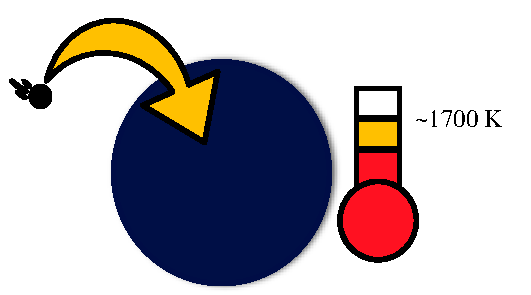
\includegraphics[width=0.45\textwidth]{img/chapter_1/kin_heat_NS.pdf}
    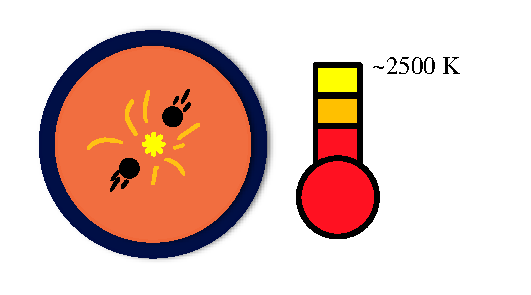
\includegraphics[width=0.45\textwidth]{img/chapter_1/ann_heat_NS.pdf}
    \caption{Illustration of DM-induced heating of compact objects. \textbf{Left:} kinetic heating due to DM scattering, raising the temperature to $\sim 1700 \K$. \textbf{Right:} Annihilation heating contributes an additional $\sim 800\K$. This image is inspired by Ref.~\cite{Raj:2017wrv_feb_Neutronstarsdark}.}
    \label{fig:cartoon_NS_heat}
\end{figure}

In order to accurately determine the limits on dark matter interactions that such an observation could place, one first requires an accurate calculation of the capture rate. However, all previous calculations relied on the formalism set up by Gould for capture in the Sun, with only minor modifications made to accommodate the extreme nature of the compact objects. 

Chapters~\ref{chapter:capture_1} and~\ref{chapter:capture_2} of this thesis are devoted to reformulating Gould's capture formalism to account for the physics specific to compact objects in a self-consistent manner. These include a relativistic treatment of the kinematics, using General Relativity to calculate the correct dark matter flux passing through the star, and accounting for Pauli blocking of the final state target using Fermi-Dirac statistics for the stellar constituents. In addition, we incorporate the internal structure of these objects by calculating the radial profiles for the relevant microscopic quantities (e.g., chemical potentials and number densities) via the adoption of a realistic equation of state.

Further considerations are required when considering dark matter interactions with the baryonic matter inside NSs. Due to the high density of the NS interior, the baryonic matter undergoes strong interactions amongst themselves and should not be treated as a free Fermi gas. Instead, adopting an equation of state that accounts for these interactions is required. These interactions modify the mass of the baryons, leading them to obtain an effective mass smaller than their vacuum mass. Furthermore, as we will see, the dark matter may interact with the baryons with momentum transfers on the order of $10\GeV$. This is high enough that the dark matter will begin to resolve the internal structure of the baryon. To account for this, the momentum dependence of the baryon form factors that are typically neglected in direct detection and solar capture must be reintroduced.

This formalism is made in preparation for a thorough analysis of the timescales involved in the dark matter heating of compact objects. The enrgy deposited in both the kinetic and annihilation heating stages does not occur instantaneously, and the timescales involved in them need to be compared to the age of the star in question. We will define kinetic heating timescale as the time required for dark matter to deposit 99\% of its initial kinetic energy into the star. For annihilation heating to occur, the dark matter must reach a state of capture-annihilation equilibrium within the stellar core. In standard calculations of this timescale, the dark matter must first become thermalised with the star. Only then can annihilations occur efficiently enough to heat the star. 


We will work with the EFT operators in Table~\ref{tab:opers_defn_full} that describe Dirac fermion dark matter interacting with Standard Model leptons. Each operator will be studied in isolation, i.e., by considering a Lagrangian that contains only one of the operators rather than a linear superposition of multiple. This way, we can analyse specific types of interactions independently, allowing us to take as model-independent an approach to phenomenology as possible. 
  
  %% 
  \graphicspath{{img/chapter_2/}}



\chapter{Compact Objects for Particle Physics}
\label{chapter:compactobjects}

\begin{synopsis}
Introduce COs, formation, structure etc...  
\end{synopsis}
%%%%%%%%%%%%%%%%%%%%%%%%%%%%%%%%%%%%%
%%%%%%%%%%%%%%%%%%%%%%%%%%%%%%%%%%%%%
%%%%%%%%%%%%%%%%%%%%%%%%%%%%%%%%%%%%%


\fixMV{Check masses in Shapiro}

The lifecycle of main sequence stars can end in various ways
depending on the progenitor star's mass. Lighter stars ($~0.6 - 10 \Msun$ at  
the onset of hydrogen burning) will eventually end their lives as a 
White Dwarf. Meanwhile, 



%%%%%%%%%%%%%%%%%%%%%%%%%%%%%%%%%%%%%
%%%%%%%%%%%%%%%%%%%%%%%%%%%%%%%%%%%%%
%%%%%%%%%%%%%%%%%%%%%%%%%%%%%%%%%%%%%
\section{Internal structure}
%%%%%%%%%%%%%%%%%%%%%%%%%%%%%%%%%%%%%
%%%%%%%%%%%%%%%%%%%%%%%%%%%%%%%%%%%%%

In this thesis we will only be considering spherically symmetric and static stars. 
The internal structure of 

For non-relativistic stars, such as our Sun, the structure equations are
rather simple, them being
\begin{align}
\frac{d M}{dr}  &= 4 \pi r^2,\\
\frac{d P }{dr} &= -\rho(r) G M(r) r^2,
\end{align}
where $M$ is the mass of the star at radius $r$, $P$ is the pressure,
and $\rho(r)$ is the density.
The first equation is known as the mass equation, and the second is the
condition for hydrostatic equilibrium. 

We are instead interested in compact objects, where the extreme densities 
of these stars 

In order to solve this system, 
The equation of state describes the relation between the pressure 
and energy of the constituent matter.


%%%%%%%%%%%%%%%%%%%%%%%%%%%%%%%%%%%%%
%%%%%%%%%%%%%%%%%%%%%%%%%%%%%%%%%%%%%
\subsection{White Dwarfs}
%%%%%%%%%%%%%%%%%%%%%%%%%%%%%%%%%%%%%
%%%%%%%%%%%%%%%%%%%%%%%%%%%%%%%%%%%%%

FMT equation of state

%%%%%%%%%%%%%%%%%%%%%%%%%%%%%%%%%%%%%
%%%%%%%%%%%%%%%%%%%%%%%%%%%%%%%%%%%%%
\subsection{Neutron Stars}
%%%%%%%%%%%%%%%%%%%%%%%%%%%%%%%%%%%%%
%%%%%%%%%%%%%%%%%%%%%%%%%%%%%%%%%%%%%


Beta Equlibrium
%%%%%%%%%%%%%%%%%%%%%%%%%%%%%%%%%%%%%
%%%%%%%%%%%%%%%%%%%%%%%%%%%%%%%%%%%%%
%%%%%%%%%%%%%%%%%%%%%%%%%%%%%%%%%%%%%
\section{Observational Status}
%%%%%%%%%%%%%%%%%%%%%%%%%%%%%%%%%%%%%
%%%%%%%%%%%%%%%%%%%%%%%%%%%%%%%%%%%%%
%%%%%%%%%%%%%%%%%%%%%%%%%%%%%%%%%%%%%

%%%%%%%%%%%%%%%%%%%%%%%%%%%%%%%%%%%%%
%%%%%%%%%%%%%%%%%%%%%%%%%%%%%%%%%%%%%
\subsection{White Dwarfs}
%%%%%%%%%%%%%%%%%%%%%%%%%%%%%%%%%%%%%
%%%%%%%%%%%%%%%%%%%%%%%%%%%%%%%%%%%%%

%%%%%%%%%%%%%%%%%%%%%%%%%%%%%%%%%%%%%
%%%%%%%%%%%%%%%%%%%%%%%%%%%%%%%%%%%%%
\subsection{Neutron Stars}
%%%%%%%%%%%%%%%%%%%%%%%%%%%%%%%%%%%%%
%%%%%%%%%%%%%%%%%%%%%%%%%%%%%%%%%%%%%



  \graphicspath{{img/chapter_3/}}
%%%%%%%%%%%%%%%%%%%%%%%%%%%%%%%%%%%%%
%%%%%%%%%%%%%%%%%%%%%%%%%%%%%%%%%%%%%
%%%%%%%%%%%%%%%%%%%%%%%%%%%%%%%%%%%%%

\chapter{Improved Treatment of Dark Matter Capture in Compact Objects}
\label{chapter:capture_1}

\begin{synopsis}
Review capture in the Sun, move to what's needed for COs in general, then specify to WDs (ions + electrons) and NS (interacting baryons)
\end{synopsis}
%%%%%%%%%%%%%%%%%%%%%%%%%%%%%%%%%%%%%
%%%%%%%%%%%%%%%%%%%%%%%%%%%%%%%%%%%%%
%%%%%%%%%%%%%%%%%%%%%%%%%%%%%%%%%%%%%

The capture rate of dark matter within celestial bodies is an essential quantity of interest throughout this work.
In this chapter, we focus on building up the formalism of dark matter 
capture within compact objects, outlining how this differs from the 
established formalism for capture in the Sun. We restrict our analysis to 
scattering off of point-like targets relevant for leptonic species, 
i.e. electrons in White Dwarfs and electrons and muons in Neutron Stars, though much of the formalism is introduced with neutron targets.



%%%%%%%%%%%%%%%%%%%%%%%%%%%%%%%%%%%%%
%%%%%%%%%%%%%%%%%%%%%%%%%%%%%%%%%%%%%
%%%%%%%%%%%%%%%%%%%%%%%%%%%%%%%%%%%%%
\section{Dark Matter Capture in the Sun}
\label{ch3:sec:solar_capture_full}
%%%%%%%%%%%%%%%%%%%%%%%%%%%%%%%%%%%%%
%%%%%%%%%%%%%%%%%%%%%%%%%%%%%%%%%%%%%
%%%%%%%%%%%%%%%%%%%%%%%%%%%%%%%%%%%%%

Before jumping into the capture formalism relevant to compact objects, it will serve us well to review the formalism laid out by Gould for capture in the Sun~\cite{Gould:1987ju_WeaklyInteractingMassive, Gould:1987ir_ResonantEnhancementsWIMP}. 

To begin, we consider the flux of dark matter particles that pass through a spherical shell a large distance $R$ from the star, where the gravitational field is negligible. For this, we need to know the distribution function of the relative velocity between the DM and the stellar constituents. 
The velocity distribution function will be spatially isotropic, and so for simplicity we will assume that the DM follows a Maxwell-Boltzmann distribution function, 
\begin{equation}
    f_\infty(\tilde{u}_\chi) d\tilde{u}_\chi= 4 \pi \left( \frac{3}{2 \pi} \right)^{3/2}\frac{\tilde{u}_\chi^2}{v_d^2} \exp\left(-\frac{3 \tilde u_\chi^2}{2 v_d^3}\right)\,d\tilde u_\chi, 
\end{equation}
where $\tilde u_\chi$ is the DM velocity in the halo, and $v_d$ is the DM halo velocity dispersion.

Taking into account the motion of the star through the halo and the thermal motion of the constituents, which are assumed to follow a Maxwell-Boltzmann distribution, gives the relative velocity between the DM and targets, $ u_\chi$. 
The distribution function for the relative velocity can be expressed as~\cite{Busoni:2017mhe_oct_Evaporationscatteringmomentum}
\begin{equation}
    f_{\mathrm{MB}}(u_\chi, \Tstar)du_\chi = \frac{u_\chi}{v_\star} \sqrt{\frac{3 }{2 \pi (v_d^2 + 3 T_\star /\mi)}} \left( e^{-\frac{3(u_\chi - v_\star)^2}{2(v_d^2 + 3 T_\star /\mi)}} - e^{-\frac{3(u_\chi + v_\star)^2}{2(v_d^2 + 3 T_\star /\mi)}} \right)du_\chi,
    \label{ch3:eq:MB_finit_T}
\end{equation}
where $v_\star$ is the star's velocity in the halo rest frame\footnote{This is the frame where the DM has an average velocity of zero.}, $T_\star$ is the temperature of the star, and $\mi$ is the mass of the target.

Returning to the large spherical shell of radius $R$, given the velocity distribution function, we can obtain the flux of DM through this surface. The rate of DM particles passing through a surface element $d\tilde{A}$ with velocity between $u_\chi$ and $u_\chi + du_\chi$, with an angle to the normal of $d\tilde{A}$ between $\tilde\theta$ and $\tilde \theta + d\tilde \theta$ and an azimuthal angle between $\tilde \phi$ and $\tilde \phi + d\tilde \phi$ is given by~\cite{Press:1985ug_Capturesungalactic}
\begin{align}
    \frac{dN_\chi}{dt} &= \frac{\rho_\chi}{m_\chi}f_{\mathrm{MB}}(u_\chi, \Tstar) \vec{u}\cdot d\vec{\tilde{A}}\, d u_\chi\, \frac{d\tilde \Omega}{4\pi}\\
    & = \frac{\rho_\chi}{m_\chi}\fMB(u_\chi, \Tstar)u_\chi \cos\tilde\theta \,d\tilde{A}\, d u_\chi\,  \frac{d\cos\tilde\theta \,d\tilde\phi}{4\pi}\\
    & = \frac{1}{4}\frac{\rho_\chi}{m_\chi}\fMB(u_\chi, \Tstar)u_\chi d\tilde{A}\, d u_\chi\,d\cos^2\tilde\theta,
\end{align}
where we have integrated over the azimuthal angle $\tilde \phi$ due to the isotropy of the system. The number density of the DM is included through the $\rho_\chi/m_\chi$ factor. 
Integrating over the area of the sphere is trivial due to isotropy, leaving us with 
\begin{align}
    \frac{dN_\chi}{dt} &= \pi \frac{\rho_\chi}{m_\chi} f(u_\chi, \Tstar)u_\chi\, d u_\chi \, d\cos^2\tilde\theta,
\end{align}
with the integration interval for $\cos^2\tilde\theta$ being $(0, 1)$.

As the DM begins to infall from this large distance $R$ to a closer distance $r$, the star's gravitational field will boost the velocity by the local escape velocity $v_e(r)$ such that
\begin{align}
    w^2_\chi(r) &= u^2_\chi + v_e^2(r),\\
    v_e^2(r) & = \frac{2 G M_\star}{R_\star} + \int_r^{R_\star} \frac{G M_\star(r')}{r'^2}\,dr'.
\end{align}
Due to the conservation of angular momentum, we can relate the angular momentum of the DM at the two distances $R$ and $r$ such that
\begin{equation}
    J_\chi = m_\chi R u_\chi \sin \tilde\theta = m_\chi r w_\chi(r) \sin\theta \leq m_\chi r w_\chi(r) \equiv J_{\mathrm{max}},
\end{equation}
where $\theta$ is the incident angle of the DM at the closer distance $r$, and we have defined the maximum angular momentum $J_{\mathrm{max}}$ corresponding to a linear DM trajectory.

Changing integration variables from $\cos^2\tilde \theta$ to $J_\chi$ allows us to write the number of DM particles passing through the shell per unit volume as
\begin{equation}
    \frac{dN_\chi}{dt} = 2\pi \frac{\rho_\chi}{m_\chi} \frac{\fMB(u_\chi, \Tstar)}{u_\chi} r^2 w_\chi^2(r) \frac{J_\chi dJ_\chi}{J^2_\mathrm{max}}\,du_\chi.\label{ch3:eq:shell_flux}
\end{equation}
The geometry of the system is shown in Fig.~\ref{ch3:fig:capturegeometry} for clarity.

\begin{figure}
    \centering
    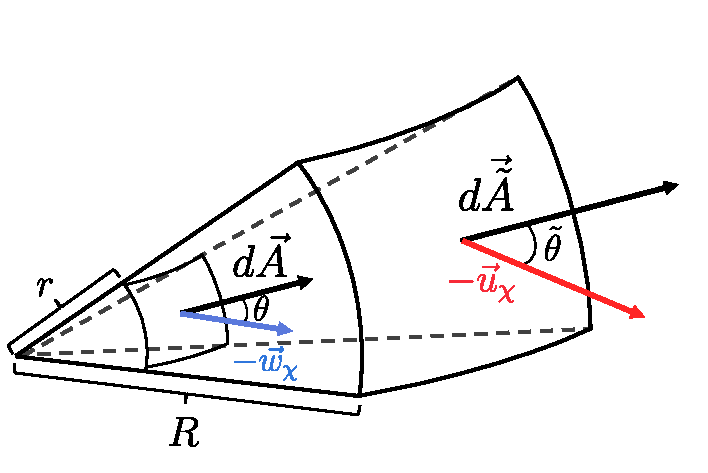
\includegraphics{img/chapter_3/capture_geometry.pdf}
    \caption{Geometry of the capture process, showing two elements of spheres with radii $r$ close to the star  }
    \label{ch3:fig:capturegeometry}
\end{figure}

The probability that the DM interacts with the constituents of the shell depends on the interaction rate, $\Omega(w_\chi)$, multiplied by the time spent in the shell, $dt = dr/\dot r$. Hence, the probability of scattering within the shell is
\begin{equation}
    \Omega(w_\chi) \frac{dr}{\dot r} = 2  \Omega(w_\chi)\frac{1}{w_\chi}\left(1 - \left(\frac{J_\chi}{r w_\chi}\right)^2 \right)^{-1/2} \Theta(J_{\mathrm{max}} - J_\chi)\,dr,\label{ch3:eq:int_prob_1}
\end{equation}
where the factor of 2 is due to the DM having two opportunities to pass through the shell, once when incoming and another after turning around\footnote{The radial velocity $\dot r$ is a standard result in orbital mechanics and can be obtained from the central force Lagrangian.}. The step-function is put in to ensure the angular momentum does not exceed its maximum allowed value. 

For a scattered DM to be considered captured, it must lose enough energy in the collision to become gravitationally bound. The rate at which a DM particle scatters from an initial velocity $w_\chi$ to a final velocity $v<v_e(r)$ is given by~\cite{Gould:1987ju_WeaklyInteractingMassive, Gould:1987ir_ResonantEnhancementsWIMP, Busoni:2017mhe_oct_Evaporationscatteringmomentum}
\begin{align}
    \Omega^{-}(w_\chi) &= \int_0^{v_e} R^-(w_\chi \rightarrow v) dv,\label{ch3:eq:down_rate_1}\\
    R^-(w_\chi \rightarrow v) & = \int n_T(r) \frac{d\sigma_{\chi T}}{dv} |\vec{w}_\chi -\vec{u}_T| f_T(u_T) \,d^3\vec{u}_T, \label{ch3:eq:diff_int_NR_gen}
\end{align}
with $R^-(w_\chi \rightarrow v)$ being the differential interaction rate, $n_T$ is the target number density, $u_T$ is the target velocity and $f_T(u_T)$ is the corresponding distribution function, and $d\sigma_{\chi T}/dv$ is the differential cross-section. The minus superscript is used to signify that this is the down scattering rate, i.e. the rate of interactions leading to the DM losing energy. 

Finally, we obtain the capture rate by multiplying Eqs.~\ref{ch3:eq:shell_flux} and~\ref{ch3:eq:int_prob_1} and integrate over the angular momentum to give the result
\begin{equation}
    C =\int_0^{R_\star} \,dr\, 4\pi r^2 \int_0^\infty\,du_\chi\, \frac{\rho_\chi}{m_\chi} \frac{\fMB(u_\chi, \Tstar)}{u_\chi} w_\chi(r)\Omega^-(w_\chi).
\end{equation}
This result is rather generic, as the choice of DM model will only dictate the form of the differential cross-section in  Eq.~\ref{ch3:eq:diff_int_NR_gen}. As written above, the distribution function for the relative velocity far from the star can be any isotropic distribution function. The MB form was chosen as it allows for a simple analytic form of the total capture rate. 

% To give a simple example, we neglect the thermal motion of the constituents, reducing the rate to
% \begin{align}
%     R^-(w_\chi \rightarrow v) = \frac{4 \mu_+^2}{\mu} n_T \frac{v}{w_\chi} \frac{d\sigma_{\chi T}}{d\cos\theta_{\mathrm{CM}}} \Theta\left(v - w\frac{|\mu_-|}{\mu_+}\right).
% \end{align}
% where $n_T$ is the local number density of the targets, and we have introduced the useful quantities $\mu$, $\mu_\pm$ that are
% \begin{equation}
%     \mu = \frac{m_\chi}{\mi}, \quad  \mu_\pm = \frac{\mu \pm 1}{2}.
% \end{equation}
% For the case of constant DM-target cross-section, we can compute the integral in Eq.~\ref{ch3:eq:down_rate_1}
% \begin{align}
%     R^-(w_\chi \rightarrow v) &= \frac{4 \mu_+^2}{\mu} n_T \frac{v}{w_\chi}\frac{\sigma_{\chi T}}{2} \Theta\left(v - w\frac{|\mu_-|}{\mu_+}\right),\\
%     \Omega^-(w_\chi) & = \frac{2\mu_+^2}{\mu} \frac{n_T \sigma_{\chi T}}{w_\chi} \left(v_e^2 - \frac{\mu_-^2}{\mu_+^2}w_\chi^2\right)\Theta\left(v_e^2 - \frac{\mu_-^2}{\mu_+^2}w_\chi^2\right).
% \end{align}

% It may be the case that the DM does not lose enough energy in a single scatter to become gravitationally bound to the star. If so, the capture probability must be modified for multi-scatter capture. \commMV{Gould and Bramante...}

%%%%%%%%%%%%%%%%%%%%%%%%%%%%%%%%%%%%%
%%%%%%%%%%%%%%%%%%%%%%%%%%%%%%%%%%%%%
%%%%%%%%%%%%%%%%%%%%%%%%%%%%%%%%%%%%%
\section{Capture in Compact Objects}
\label{ch3:sec:captrue_new_full}
%%%%%%%%%%%%%%%%%%%%%%%%%%%%%%%%%%%%%
%%%%%%%%%%%%%%%%%%%%%%%%%%%%%%%%%%%%%
%%%%%%%%%%%%%%%%%%%%%%%%%%%%%%%%%%%%%

Having reviewed the capture process in non-relativistic stars, we can begin discussing the necessary modifications required when considering relativistic stars. In this section, we consider the two major modifications that need to be made: 
\begin{itemize}
    \item The corrections from General Relativity due to the extreme gravitational fields. This ultimately alters the flux of DM passing through the star, boosting it through gravitational focusing.
    \item Accounting for the relativistic and degenerate nature of the star's constituents in the interaction rate.
\end{itemize}

The former is generic to neutron stars and white dwarfs, while the latter is required for all NS constituents, but only the electrons in a WD are degenerate and relativistic. The ions of the WD are non-relativistic and non-degenerate and, hence, can the solar capture formalism can be applied in this case. 

%%%%%%%%%%%%%%%%%%%%%%%%%%%%%%%%%%%%%
%%%%%%%%%%%%%%%%%%%%%%%%%%%%%%%%%%%%%
\subsection{General Relativistic Corrections to the Capture Rate}
\label{ch3:subsec:GR_corr_capture}
%%%%%%%%%%%%%%%%%%%%%%%%%%%%%%%%%%%%%
%%%%%%%%%%%%%%%%%%%%%%%%%%%%%%%%%%%%%

Far from the star, the physics is the same as in the previous section. The deviations arise as the DM falls into he gravitational potential of the star. We begin by following the DM along its trajectory, moving from a distance $R\gg R_\star$ to a closer distance $r$. Hence, we are working in the DM rest frame and calculating the rate at which the DM passes through the shell \textit{per unit of proper time}, $\tau$. The proper time interval is related to the metric through
\begin{equation}
    d\tau^2 = B(r) dt^2 - A(r) dr^2 - r^2 d\Omega^2,
\end{equation}
with $B(r)$ and $A(r)$ defined in Chapter~\ref{chapter:compactobjects}. 

Following the same arguments as in the non-relativistic case, the flux of DM passing through the shell is 
\begin{equation}
    \frac{d N_\chi}{d\tau} = 2\pi \frac{\rho_\chi}{m_\chi}\frac{\fMB(u_\chi)}{u_\chi}\,du_\chi\,\frac{J_\chi \, dJ_\chi}{m_\chi^2},
\end{equation}
which takes the same form as Eq.~\ref{ch3:eq:shell_flux}, with the physical difference being that this is the rate with respect to the proper time. Additionally, as we will be considering cold stars, we take the $\Tstar\rightarrow 0$ limit of the DM-target relative velocity distribution, such that 
\begin{align}
    f_{\mathrm{MB}}(u_\chi) & = \lim_{\Tstar\rightarrow 0}f_{\mathrm{MB}}(u_\chi, \Tstar)\\
    & = \frac{u_\chi}{v_\star} \sqrt{\frac{3 }{2 \pi (v_d^2 + 3 T_\star /\mi)}} \left( e^{-\frac{3(u_\chi - v_\star)^2}{2(v_d^2 + 3 T_\star /\mi)}} - e^{-\frac{3(u_\chi + v_\star)^2}{2(v_d^2 + 3 T_\star /\mi)}} \right),
    \label{ch3:eq:MB}
\end{align}

The probability that DM scatters within the shell and is captured is $2\hat{\Omega}^-(r) d\tau$,
where $\hat{\Omega}^-(r)$ is the interaction rate with respect to the proper time, and $d\tau$ is the proper time taken to move from coordinate $r$ to $r + dr$. The factor of 2 once again accounts for the DM crossing the shell twice per orbit. For calculation purposes, we need to relate this to the interaction rate seen by a distant observer, $\Omega^-(r)$, that is done through
\begin{equation}
    \hat{\Omega}^-(r) d\tau = \frac{1}{\sqrt{g_{tt}}}\Omega^-(r)d\tau= \frac{1}{\sqrt{B(r)}}\Omega^-(r)d\tau.
\end{equation}
Now, the proper time that the DM spends inside a shell of thickness $dr$ will be\footnote{See Appendix~\ref{appendix:kin_heating} for the derivation of $\dot r = \frac{dr}{dt}$.}
\begin{equation}
    d\tau = \left( \frac{d\tau}{dt}\right) dt = B(r) \frac{dr}{\dot r} = \frac{\sqrt{B(r)} dr}{\sqrt{\frac{1}{A(r)} \left[ 1 - B(r)\left( 1 + \frac{J_\chi^2}{m_\chi^2 r^2} \right) \right]}}.
\end{equation}

The differential capture rate can then be written as 
\begin{equation}
    dC =  2\pi  \frac{\rho_\chi}{m_\chi}\frac{\fMB(u_\chi)}{u_\chi}\,du_\chi\,\frac{dJ^2_\chi}{m_\chi^2} \frac{\Omega^-(r)\sqrt{A(r)} \,dr}{\sqrt{1 - B(r)\left( 1 + \frac{J_\chi^2}{m_\chi^2 r^2} \right)}}.
\end{equation}
As the total number of targets in the star, $N_T$, needs to satisfy
\begin{equation}
    N_T = \int_0^{R_\star} 4\pi r^2 n_T(r)\sqrt{A(r)}\,dr,
\end{equation}
where $n_T(r)$ is the number density that appears in the interaction rate, we absorb the factor $\sqrt{A(r)}$ into the definition of $n_T(r)$, such that $\Omega^-(r)\sqrt{A(r)}\rightarrow \Omega^-(r)$. This is due to the number densities obtained by solving the TOV equations already account for the $\sqrt{A(r)}$ factor. 

As before, we have $w_\chi^2(r) = u_\chi^2 + v_e^2(r)$, however as the escape velocity will be significantly larger than the ambient DM velocity far from the star, we can safely approximate $w_\chi^2(r)\approx v_e^2(r)$. 
In the relativistic case, the escape velocity can be defined as
\begin{equation}
    v_e^2(r) = \left(\frac{dl}{d\tau}\right)^2 = A(r) \left(\frac{dr}{d\tau}\right)^2 + r^2 \left(\frac{d\phi}{d\tau}\right)^2 = 1 - B(r),
    \label{ch3:eq:vesceq}
\end{equation}
where $dl$ is a length element. 
The large boost from the escape velocity also removes the $u_\chi$ dependence in the kinematics of the interactions and allows us to perform the integration over the initial DM velocity, yielding an overall factor of
\begin{equation}
    \int_0^\infty \frac{\fMB(u_\chi)}{u_\chi} du_\chi = \frac{1}{v_\star}\erf\left(\sqrt{\frac{3}{2}}\frac{v_\star}{v_d}\right).
\end{equation}

To integrate over $J^2_\chi$, we need the maximum angular momentum the DM can achieve as it passes through the shell. This can be obtained by requiring the argument of the radical above to remain positive, giving
\begin{equation}
    J_\mathrm{max} = \sqrt{\frac{1 - B(r)}{B(r)}} m_\chi r.
\end{equation}
The factor of $1/\sqrt{B}$ arises due to the gravitational focusing of the incoming flux of DM~\cite{Kouvaris:2007ay_WIMPAnnihilationCooling}.
% The angular momentum is given by
% \begin{equation}
%     J_\chi = m_\chi r^2\frac{d\phi}{d\tau}  \leq \frac{m_\chi}{\sqrt{B(r)}} r w_\chi(r) = J_\mathrm{max},
% \end{equation}
% This can be obtained by requiring that the contents of the square root above remain positive, giving
% \begin{equation}
%     J_\mathrm{max}^2 = \frac{1-B(r)}{B(r)} m_\chi^2 r^2,
% \end{equation}

Putting everything together, and integrating over the radius of the star, we are left with the final result for the capture rate of
\begin{equation}
    C =\frac{4\pi}{v_\star}\frac{\rho_\chi}{m_\chi} \erf\left(\sqrt{\frac{3}{2}}\frac{v_\star}{v_d}\right) \int_0^{R_\star}  r^2\frac{\sqrt{1 - B(r)}}{B(r)}\Omega^-(r)\,dr.
    \label{ch3:eq:cap_rel_full_1}
\end{equation}
All that remains is determining the form of the interaction rates for relativistic energies.


%%%%%%%%%%%%%%%%%%%%%%%%%%%%%%%%%%%%%
%%%%%%%%%%%%%%%%%%%%%%%%%%%%%%%%%%%%%
\subsection{Geometric Limit and Threshold Cross-Section}
\label{ch3:subsec:geom_lim_threshold_xs}
%%%%%%%%%%%%%%%%%%%%%%%%%%%%%%%%%%%%%
%%%%%%%%%%%%%%%%%%%%%%%%%%%%%%%%%%%%%

In the previous section, we derived an expression for the capture rate assuming that the DM is captured after a single scatter, and that it only scatters once along its orbit through the NS. This first assumption is true for DM light enough to lose enough energy in this single interaction, which for nucleon targets turns out to be $m_\chi\lesssim 10^6\GeV$. The latter assumption is a statement that we are working in the optically thin regime, such that the cross-section is much less than the ``threshold cross-section'', $\sigmath$. The value of the threshold cross-section is defined as the cross-section for which the capture rate evaluated in the optically thin regime is equal to the geometric limit \cite{Bell:2018pkk_sep_HeatingNeutronStars},  
%
\begin{equation}
C_\mathrm{geom} =  \frac{\pi R_\star^2(1-B(R_\star))}{v_\star B(R_\star)} \frac{\rho_\chi}{m_\chi} \erf\left(\sqrt{\frac{3}{2}}\frac{v_\star}{v_d}\right).
\label{ch3:eq:capturegeom}
\end{equation}
% 
This is the capture rate for which the entire flux of DM passing through the surface of the star is captured at the surface. Hence, it serves as an upper bound to the capture rate, with cross-sections greater than $\sigmath$ saturating the capture rate to this value.
Note the $1/B(\Rstar)$ factor in the equation above. In stars and planets where classical Newtonian mechanics can be applied, gravitational focusing would result in a factor  $v_{esc}^2/\vstar =  (1-B(\Rstar))/\vstar$ in Eq.~\ref{ch3:eq:capturegeom}, where we have used Eqs.~\ref{ch3:eq:vesceq} and \ref{ch2:eq:B_boundary_condition}. 
In neutron stars, on the other hand, general relativity introduces an additional factor of $1/B(\Rstar)$, which can be obtained from the derivation of the flux of DM particles accreted to a NS with a Schwarzschild metric (Eq.~\ref{ch3:eq:cap_rel_full_1})~\cite{Goldman:1989nd_WeaklyInteractingMassive,Kouvaris:2007ay_WIMPAnnihilationCooling}.

For scattering on neutrons, the threshold cross-section is approximately
\begin{align}
\sigma_{th} =  \begin{cases}
\, \sigma_\mathrm{ref} \frac{\GeV}{m_\chi}, \quad &m_\chi \lesssim 1\GeV \quad \ \ \text{ (Pauli blocking  regime)}, \\
\, \sigma_\mathrm{ref}, \quad &1\GeV \lesssim m_\chi \lesssim 10^6\GeV,  \\
\, \sigma_\mathrm{ref} \frac{m_\chi}{10^6\GeV}, \quad &m_\chi\gtrsim 10^6\GeV \quad  \text{(Multiscattering regime)},
\end{cases}
\label{ch3:eq:sigmath}
\end{align}
where we take the canonical value of
\begin{equation}
    \sigma_\mathrm{ref}\sim 1.7 \times 10^{-45}\cm^2,
\end{equation}
which assumes the NS is a solid sphere such that $\sigmaref\sim m_n \pi \Rstar^2/\Mstar$ with $m_n$ the neutron mass.

For scattering off other targets, Pauli blocking is relevant for $\qomax \lesssim  \mu_{\rm target}$ 
while multi-scattering is relevant for $m_\chi \gtrsim \qomax/v_{\star}^2$, where $\qomax$ is the maximum energy transfered in a collision, as will be discussed later.  In addition, because the other target species have a lower abundance than neutrons, the reference cross-section, $\sigma_\mathrm{ref}$, will be higher. The values of $\sigma_{th}$ in Eq.~\ref{ch3:eq:sigmath}, and their regions of applicability, can thus be altered appropriately for other target species of interest.

%%%%%%%%%%%%%%%%%%%%%%%%%%%%%%%%%%%%%
%%%%%%%%%%%%%%%%%%%%%%%%%%%%%%%%%%%%%
\subsection{Interaction Rate for Relativistic Energies and Degenerate Targets}
\label{ch3:subsec:int_rate_degen_rel}
%%%%%%%%%%%%%%%%%%%%%%%%%%%%%%%%%%%%%
%%%%%%%%%%%%%%%%%%%%%%%%%%%%%%%%%%%%%

Our next goal is to write down an interaction rate suitable for describing the interactions between relativistic particles and account for the degeneracy of the target species. This will be achieved by modifying the non-relativistic interaction rate of Eq.~\ref{ch3:eq:down_rate_1} through the use of relativistic kinematics and the use of Lorentz invariant quantities, and the correct distribution functions for degenerate fermion targets.

As shown in Eqs.~\ref{ch3:eq:down_rate_1} and~\ref{ch3:eq:diff_int_NR_gen}, the interaction rate between non-relativistic, non-degenerate species $i$ can be expressed as
\begin{equation}
    \Omega^{-}(r) = \int dv \frac{d\sigma}{dv} |\vec{w}_\chi -\vec{u}_i| n_i(r) \fMB(u_i)d^3u_i.
    \label{ch3:eq:NR_int_rate_simple}
\end{equation}
First, we address the degeneracy of the targets by exchanging the Maxwell-Boltzmann distribution function for a Fermi-Dirac (FD) distribution, $\fFD(\Ei,r)$, via the replacement
\begin{equation}
    n_i(r) \fMB(u_i)d^3 u_i \rightarrow \frac{g_s}{(2\pi)^3}\fFD(\Ei, r),
    \label{ch3:eq:number_density_replacement}
\end{equation}
where $g_s = 2$ is the number of spin states of the target species, $p$ is the 3-momentum of the incoming target, and $\Ei$ is its corresponding energy. The radial dependence of the FD distribution stems from its implicit dependence on the chemical potential of the target. Rewriting this expression in a more computationally friendly manner in terms of the relevant kinematic quantities results in 
\begin{equation}
    \frac{g_s}{(2\pi)^3}\fFD(\Ei, r) = \frac{p \Ei}{2\pi^2}\fFD(\Ei, r) d\Ei d\cos\theta_{uw},
    \label{ch3:eq:free_Fermi_number}
\end{equation}
where we have expressed the angular component of the $d^3 p$ differential in terms of the angle between the incoming DM and target. This angle can be traded for the more useful quantity $s$, the centre of mass energy through
\begin{equation}
    \frac{d\cos\theta_{uw}}{ds} = \frac{1}{2 p p_\chi} = \frac{1}{2 p \sqrt{E_\chi^2 - m_\chi^2}} = \frac{1}{2 p m_\chi}\sqrt{\frac{B(r)}{1 - B(r)}},
\end{equation}
as the initial DM energy is $E_\chi = m_\chi/\sqrt{B(r)}$.

Next, we calculate the initial relative velocity, $|\vec{w}_\chi -\vec{u}_i|$, using relativistic kinematics, expressing it in terms of the Mandalstam $s$, 
\begin{equation}
    |\vec{w}_\chi -\vec{u}_i| = \frac{\sqrt{s^2 - 2 s (1 + \mu^2)\mi^2 + (1 - \mu^2)^2 \mi^4}}{s - (1 + \mu^2) \mi^2},
\end{equation}
where $\mu = m_\chi/\mi$.

Given that it is most common to present the relativistic differential scattering cross-section $d\sigma/d\cos\thetacm$ as a function of the Mandalstam variables $s$ and $t$, with $\thetacm$ the centre of mass frame scattering angle, we make the replacement
\begin{equation}
    dv \frac{d\sigma}{dv} = dt\frac{d\sigma}{dt} = dt \frac{d\sigma}{d\cos\thetacm}\frac{d\cos\thetacm}{t}.
\end{equation}
The final Jacobian factor can be expressed as
\begin{equation}
    \frac{d\cos\thetacm}{dt} = \frac{2s}{s^2 - 2 s (1 + \mu^2)\mi^2 + (1 - \mu^2)^2 \mi^4},
\end{equation}
for the elastic scattering we consider here.

Finally, we note that the first application of this capture formalism was for neutron targets, with the analysis completed before we had considered the additional effects from the form factors and strong interactions discussed in subsection~\ref{ch1:subsec:quark_to_nucleon_EFT}. These effects will be incorporated into this formalism in a self-consistent way next chapter. The initial approach that was taken to account for the fact that we are using realistic neutron number density profiles, despite the expression in Eq.~\ref{ch3:eq:number_density_replacement} being for a free Fermi gas, is to introduce a correction factor as in Ref.~\cite{Garani:2018kkd_may_NewAnalysisNeutron},
\begin{equation}
    \zeta(r) = \frac{n_i(r)}{n_\mathrm{free}(r)},
\end{equation}
where $n_\mathrm{free}(r)$ is obtained by integrating Eq.~\ref{ch3:eq:free_Fermi_number} over all phase space. In the zero-temperature approximation, the result is

\begin{equation}
    n_\mathrm{free}(r) = \frac{1}{3\pi^2}\left[ \kinFi(r)(2\mi + \kinFi(r))\right]^{3/2}.
\end{equation}

Compiling everything together leads to the final expression for the interaction rate being
\begin{equation}
    \begin{split}
        \Omega^-(r) = \int dt\,d\Ei\,ds\,\zeta(r) \frac{d\sigma}{d\cos\thetacm}\frac{\Ei}{2\pi^2 \mi}&\sqrt{\frac{B(r)}{1 - B(r)}} \frac{s}{\beta(s)\gamma(s)}\\
        &\times\fFD(\Ei, r)(1 - \fFD(\Ei', r)),
    \end{split}
    \label{ch3:eq:int_rate_capture_full}
\end{equation}
where we have introduced the helper functions
\begin{align}
    \beta(s) & = s - (\mi^2 + m_\chi^2),\\
    \gamma(s) & = \sqrt{\beta^2(s) - 4 \mi^2 m_\chi^2}.
\end{align}
We have also introduced the Pauli blocking factor, $1 - \fFD(\Ei', r)$, to account for the phase space available to the final state target. The energy of this final state particle, $\Ei'$, is in general a messy function of $\Ei$, $t$, $s$, and $r$, and can be obtained from the kinematics of the scattering. This result is presented in Appendix~\ref{app:kinematics}.

The integration intervals are 
\begin{align}
    t_\mathrm{min} & = - \frac{\gamma(s)}{s},\\
    t_\mathrm{max} & = 0,\\
    s_\mathrm{min} & = \mi^2 + m_\chi^2 + 2 \frac{\Ei \mchi}{\sqrt{B(r)}} - 2\mchi\sqrt{\frac{1 - B(r)}{B(r)}} \sqrt{\Ei^2 - \mi^2}, \\
    s_\mathrm{max} & = \mi^2 + m_\chi^2 + 2 \frac{\Ei \mchi}{\sqrt{B(r)}} + 2\mchi\sqrt{\frac{1 - B(r)}{B(r)}} \sqrt{\Ei^2 - \mi^2}, \\
    E_{i,\mathrm{min}} & = \mi,\\
    E_{i,\mathrm{max}} & = \frac{\mi}{\sqrt{B(r)}}.
\end{align}

As we will be dealing with NSs at low temperatures, we can take the $\Tstar\rightarrow 0$ limit and replace the FD functions with step functions, 
\begin{align}
    \fFD(\Ei, r) &\rightarrow \Theta(\kinFi(r) +\mi - \Ei),\\
    1 - \fFD(\Ei', r) & \rightarrow  \Theta(\Ei'-\mi - \kinFi(r) ).
\end{align}
The first step function can be used to further restrict the $\Ei$ integration interval to be $[\mi, \mi + \kinFi(r)]$. In practice, we work with the kinetic energies of the targets rather than their total energy, as this is the quantity that directly changed in the interactions. Therefore, unless otherwise specified, we will take $\Ei$ to mean the target kinetic energy, with the integration range being $0\le \Ei\le \kinFi$.

This expression resembles that of Ref.~\cite{Garani:2018kkd_may_NewAnalysisNeutron}, but uses a relativistic formalism instead. In Appendix~\ref{sec:weakfieldlimit}, we show that Eq.~\ref{ch3:eq:int_rate_capture_full} reduces to the classical expression for the interaction rate in the non-relativistic limit. 


%%%%%%%%%%%%%%%%%%%%%%%%%%%%%%%%%%%%%
%%%%%%%%%%%%%%%%%%%%%%%%%%%%%%%%%%%%%
%%%%%%%%%%%%%%%%%%%%%%%%%%%%%%%%%%%%%
\section{The Differential Interaction Rate}
\label{ch3:sec:diff_int_rate}
%%%%%%%%%%%%%%%%%%%%%%%%%%%%%%%%%%%%%
%%%%%%%%%%%%%%%%%%%%%%%%%%%%%%%%%%%%%
%%%%%%%%%%%%%%%%%%%%%%%%%%%%%%%%%%%%%

In the previous section, we have calculated the interaction rate, $\Omega^-(r)$, assuming the initial DM energy takes its pre-capture value, $E_\chi = \mchi /B(r)$. However, we are also interested in an expression for the interaction rate valid for arbitrary DM energy. This will be required when we consider capture via multiple scatterings, and it will also be necessary to study the subsequent scattering interactions that follow capture and lead to the DM thermalising within the NS.
In principle, it is possible to calculate this rate numerically by binning $\Omega^-$, Eq.~\ref{ch3:eq:int_rate_capture_full}, in the energy loss, i.e. multiplying $\Omega^-$ by $\frac{1}{E_i-E_j}\Theta(E_i+\Ei-\Ei')\Theta(\Ei'-\Ei-E_j)$ and integrating over the bin $[E_j,E_i]$. 
However, it is possible to derive analytic expressions for the differential rate, valid in the zero-temperature approximation. To do so, we use the definition of the scattering rate in Ref.~\cite{Reddy:1997yr_Neutrinointeractionshot,Bertoni:2013bsa_dec_DarkMatterThermalization} 
\begin{equation}
    \begin{split}
        \Gamma^-(E_\chi) &= 2\int \frac{d^3k'}{(2\pi)^3}\int \frac{d^3p}{(2\pi)^3}\int \frac{d^3p'}{(2\pi)^3} \frac{|\overline{M}|^2}{(2E_\chi)(2E'_\chi)(2\Ei)(2\Ei')}\\
        &\hspace{4em}\times(2\pi)^4\delta^4\left(k_\mu+p_\mu-k_\mu'-p_\mu'\right) \fFD(\Ei)(1-\fFD(\Ei')),
    \end{split}
\label{ch3:eq:scattrate}
\end{equation}
where $\Msq$ is the squared matrix element,
$k^\mu=(E_\chi,\vec{k})$ and $k^{'\mu}=(E'_\chi,\vec{k'})$ are the DM initial and final momenta, and $p^\mu=(\Ei,\vec{p})$ and $p^{'\mu}=(\Ei',\vec{p'})$ are the target particle initial and final momenta, respectively.
To see that $\Gamma^-$ is indeed the same as $\Omega^-$ in Eq.~\ref{ch3:eq:int_rate_capture_full}, multiply and divide by
$v_{rel}=|\vec{w}-\vec{u}_i|$ to reintroduce the quantum field theoretic definition of differential cross-section, 
\begin{align}
    d\sigma & = \frac{\Msq}{2 E_\chi 2\Ei|\vec{w} - \vec{u}_i|}d^2\Pi_\mathrm{LIPS},\\
    d^2\Pi_\mathrm{LIPS} &= \frac{1}{2E'_\chi}\frac{d^3 k'}{(2\pi)^3}\frac{1}{ 2\Ei'}\frac{d^3 p'}{(2\pi)^3}(2\pi)^4\delta^4(k_\mu + p_\mu - k'_\mu - p'_\mu),\\
    \implies\frac{d\sigma}{d\cos\thetacm} &= \frac{1}{16 \pi}\frac{\beta(s)}{2 s \beta(s) - \gamma^2(s)}\Msq,
\end{align}
where $d^2\Pi_\mathrm{LIPS}$ is the 2-body Lorentz invariant phase space.

The advantage of Eq.~\ref{ch3:eq:int_rate_capture_full} is that it can be used to calculate the capture rate for any interaction given the differential cross-section. The disadvantage is that this computation has to be evaluated numerically, which can be computationally intensive. For this reason, shall now use Eq.~\ref{ch3:eq:scattrate} to derive analytic expressions that will allow us to speed up computations and, in addition, calculate the shape of the interaction rate as a function of the energy loss. 

The interaction rate for $d\sigma \propto s^m t^n$ is 
\begin{align}
    \begin{split}
        \Gamma^{-}(E_\chi)- & = \sum_{n,m}  \frac{(-1)^n \alpha_{n,m}}{128\pi^3 E_\chi k }\int_0^{E_\chi -m_\chi} dq_0\int \frac{dt_E t_E^n}{(t_E + q_0^2)^{m+\frac{1}{2}}}\\
        &\hspace{4em}\times\sum_{r=0}^m \mathcal{V}_{m,r}\sum_{j = 0}^r\binom{r}{j} \kinFi^{r-j}  \frac{(-1)^{j} q_0^{j+1}}{j+1} h_j\left( \frac{\Ei^{t^-} - \kinFi}{q_0}\right),
    \end{split}
    \label{ch3:eq:gamma_full_text}
\end{align}
for elastic scattering with $t_E=-t=q^2-q_0^2$, where $q_0=\Ei'-\Ei$ is the DM energy loss, 
\begin{equation}
\Ei^{\, t^{-}} = -\left(m_n+\frac{q_0}{2}\right) + \sqrt{\left(m_n+\frac{q_0}{2}\right)^2+\left(\frac{\sqrt{q^2-q_0^2}}{2}-\frac{m_n q_0}{\sqrt{q^2-q_0^2}}\right)^2}, 
\end{equation}
is the minimum energy of the neutron before the collision, obtained from kinematics,  and $h_j(x)$ is a step function with a smooth transition, 
\begin{equation}
    h_j(x) = \begin{cases}
        & 0, \quad x >0\\
        & (-x)^{j+1},\quad -1<x <0\\
        & 1,\quad x<-1
    \end{cases}.
\end{equation}
The full derivation of this interaction rate can be found in Appendix~\ref{app:interaction_rates}. 
Our result for $\Gamma^-$ is an extension of that presented in Ref.~\cite{Bertoni:2013bsa_dec_DarkMatterThermalization}, where the interaction rate was calculated only in the case of low energy and a constant matrix element. It is valid at all energy ranges.
The differential interaction rate $\frac{d\Gamma}{d q_0}(E_\chi,q_0)$ is then just the integrand of Eq.~\ref{ch3:eq:gamma_full_text}.
We will use $\frac{d\Gamma}{d q_0}$ to obtain normalised shapes for the differential interaction spectrum, while we will use $\Omega^-$ when we need the total interaction rate, such as in the capture rate. 


%%%%%%%%%%%%%%%%%%%%%%%%%%%%%%%%%%%%%%%
\begin{figure}[t!bp]
    \centering
    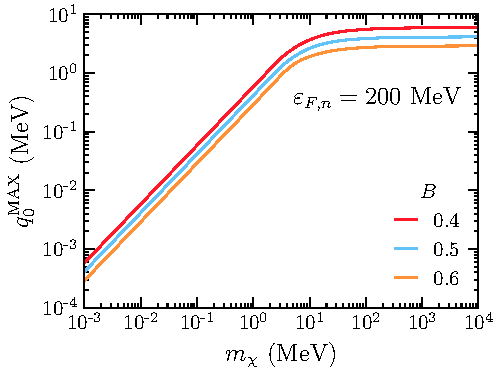
\includegraphics[width = 0.495\textwidth]{capture_1/q0max_mdm.pdf}
    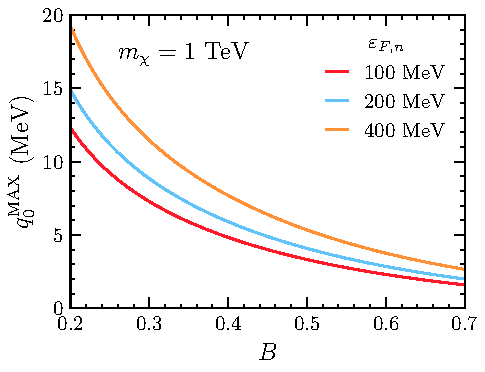
\includegraphics[width = 0.495\textwidth]{capture_1/q0max_B.pdf}

    \caption{Left: $\qomax$ vs. $m_\chi$ for $\kinFn=200\MeV$ and different values of B. 
    Right: $\qomax$ as a function of $B$ for different values of $\kinFi$ and $m_\chi=1\TeV$.}
    \label{ch3:fig:q0max}
\end{figure}
%%%%%%%%%%%%%%%%%%%%%%%%%%%%%%%%%%%%%%

%%%%%%%%%%%%%%%%%%%%%%%%%%%%%%%%%%%%%%
\begin{figure}[t!bp]
    \centering
    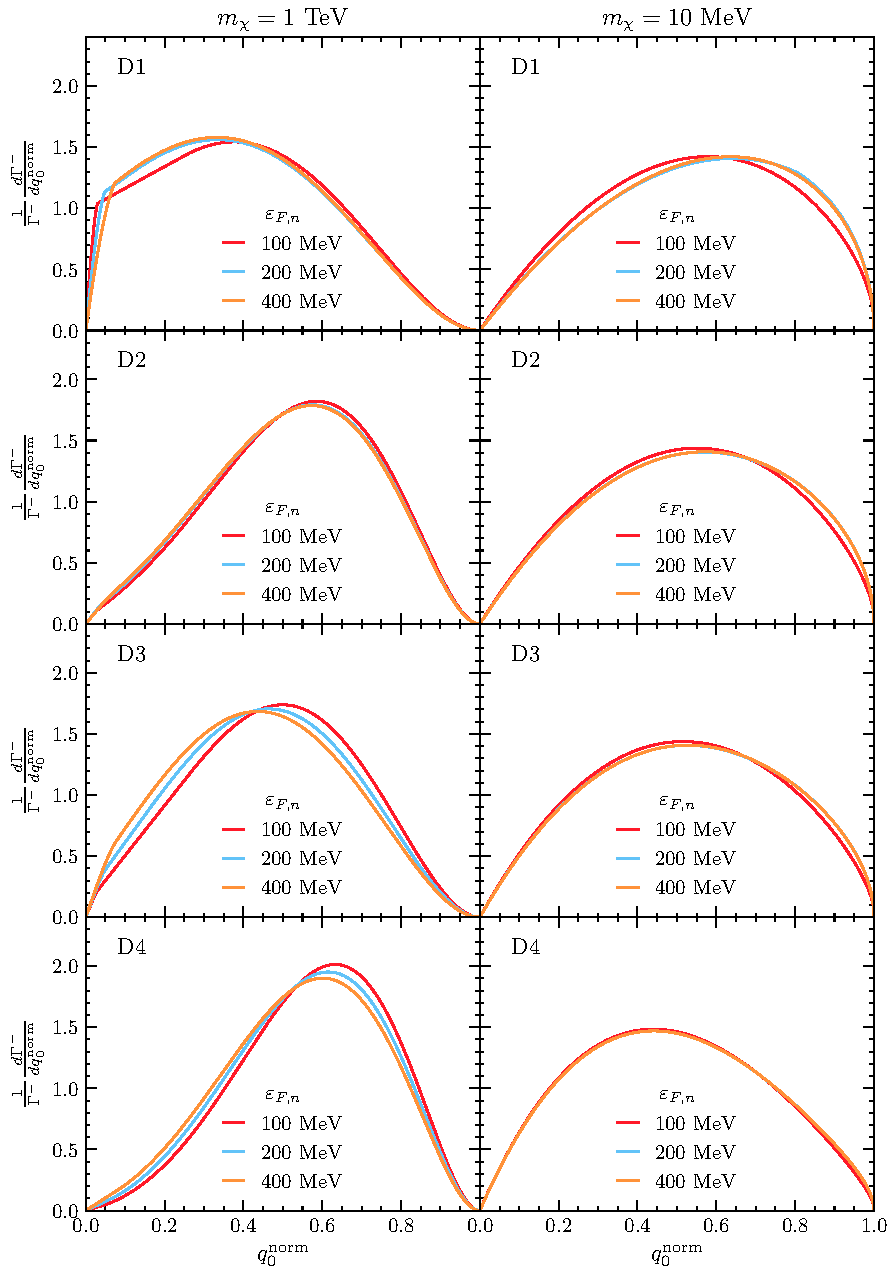
\includegraphics[width = 0.87\textwidth]{capture_1/norm_diff_intrate.pdf}    
    \caption{Normalised differential interaction rates $\frac{1}{\Gamma}\frac{d\Gamma}{d\qonorm}$ as a function of $\qonorm$ for different values of $\kinFn$, $m_\chi=1\TeV$ (left) and $m_\chi=10\MeV$ (right), $B=0.5$ and  operators D1 (first row), D2 (second row), D3 (third row) and D4 (fourth row). Profiles do not depend on $m_\chi$ in the limits $m_\chi\gg m_n$ (left) and $m_\chi\ll m_n$ (right).  }
    \label{ch3:fig:diffintratesd14}
\end{figure}
%%%%%%%%%%%%%%%%%%%%%%%%%%%%%%%%%%%%%%


Kinematics, and the phase space allowed by $h_j(x)$ in Eq.~\ref{ch3:eq:gamma_full_text}, determine the maximum energy that a DM particle can lose in a single scattering interaction, $\qomax$. The details of how to obtain $\qomax$ are given in Appendix~\ref{app:subsec:down_scatter_derivation}.
For DM capture, the value of $\qomax$ depends primarily on the DM mass, as is illustrated in the left panel of Fig.~\ref{ch3:fig:q0max}. We can see that for low $m_\chi$, $\qomax\propto m_\chi$, while, for $m_\chi\gg m_n$, it plataues to values between $\qomax\sim 3 - 6 \GeV$. 
%
Both $\qomax$ and $\frac{d\Gamma}{dq_0}$ also depend on $\kinFn$ and $B$. Changing $\kinFn$ has a very mild effect on the value of $\qomax$ (see right panel of Fig.~\ref{ch3:fig:q0max}) and on the shape of the normalised spectrum (see Fig.~\ref{ch3:fig:diffintratesd14}). On the other hand, increasing $B$ has the main effect of reducing   $\qomax$ (see right panel of Fig.~\ref{ch3:fig:q0max}), but only a mild effect on the shape of the profile expressed as a function of the normalised energy loss 
\begin{equation}
    \qonorm = \frac{q_0}{\qomax}. 
\end{equation}

We apply our results for $\frac{d\Gamma}{d q_0}$ to DM-neutron interactions, and in particular those with differential cross-sections that depend only on the transferred momentum $t=(k^\mu-k^{'\mu})^2$ and not on the centre of mass energy $s=(p^\mu+k^\mu)^2$.

In Fig.~\ref{ch3:fig:diffintratesd14} we show the normalised differential rates as a function of $\qonorm$ for the four operators D1-D4. The left-hand panels are in the limit $m_\chi\gg m_n$. We can observe that D1 has a softer spectrum, while the D2 and D4 spectra peak towards higher values of $q_0$. Varying the chemical potential $\kinFn$ has a very mild effect, shifting the spectrum to lower values of $q_0$ with increasing values of $\kinFn$.
Note that at small values of $\qonorm$ there is a sudden change in the slope of the normalised differential rate, which occurs for all operators but is more evident in D1 (top left panel). This is due to the zero temperature approximation, implicit in Eq.~\ref{ch3:eq:gamma_full_text}, where Heaviside functions were used to approximate FD distributions (see Appendix~\ref{app:subsec:down_scatter_derivation}); using a finite temperature would produce a smoother spectrum at small $\qonorm$. 

In the right-hand panels of Fig.~\ref{ch3:fig:diffintratesd14}, we explore the low DM mass region $m_\chi\ll m_n$. 
In this case, all operators give rise to similar profiles, the sole difference being that the peak of the profile is now shifted to lower  $\qonorm$ for D4 in contrast to D1, with intermediate values for D2 and D3. This is a consequence of Pauli blocking, with this effect depending on the specific power of $t$ that dominates the spectrum. Profiles with lower $n$ ($d\sigma\propto t^n$) peak at higher $\qonorm$ (see Fig.~\ref{ch3:fig:diffintratesd14}, right panels). For D4 we have $\Msq\propto t^2$, while the matrix elements of D2 and D3 are linear combinations of $t$ and $t^2$, and D1 is a combination of all powers of $t$. Comparing the right panels of Fig.~\ref{ch3:fig:diffintratesd14} with Fig.~\ref{app:fig:diffgamma}, we observe that the lowest power of $t$ determines the shape of the final differential interaction rate. Finally, varying $\kinFn$ has a very mild effect, this time shifting the spectrum mostly to higher values of $q_0$ for higher $\kinFn$.

The fact that the lowest power of $t$ dictates the features of the differential interaction rate is true also for the interactions that have a dependence on $s$. As such, by understanding the properties of the interaction rates with $\Msq\propto t^n$, we can understand the rates for all the operators in Table.~\ref{ch1:tab:opers_defn_full}.


%%%%%%%%%%%%%%%%%%%%%%%%%%%%%%%%%%%%%%%%%
\subsection{Pauli Blocking}
\label{ch3:subsec:PB_cap}
%%%%%%%%%%%%%%%%%%%%%%%%%%%%%%%%%%%%%%%%%
% The DM interaction rate, Eq.~\ref{ch3:eq:scattrate}, is proportional to the number of target particles (nucleons/leptons) in the initial state with energy $\Ei$, and to the number of available final states with energy $\Ei+q_0$. 

The DM interaction rate, Eq.~\ref{ch3:eq:scattrate}, will be proportional to the number of target particles available to scatter off. Classically, this is the total number of targets within the star. However, the quantum degeneracy of the species within compact objects, due to the extreme densities, leads to a reduction in the number of available initial state target particles the DM can scatter off.
To understand this, consider the $T\rightarrow 0$ approximation, in which all initial states with energies $\Ei < \kinFi$ are occupied. These states are known as the ``Fermi sea". In order for the DM to scatter off one of these states, it must impart enough energy to kick the target out of the Fermi sea, such that 
\begin{equation}
    \Ei' = \Ei + q_0 > \kinFi,
\end{equation}
imposing a lower limit on the energy transfer required for an interaction to take place. This effectively reduces the number of available targets to only those with kinetic energies between $\kinFn - q_0$ and $\kinFi$. 
This suppression of the initial state phase space is known as Pauli blocking (PB), and is a completely quantum phenomenon.
In this limit, we necessarily have $\Gamma^-\rightarrow 0$ for $q_0\rightarrow 0$. 
It is also worth noting that Pauli blocking only affects the interaction rate when $q_0\le \kinFn$.


%%%%%%%%%%%%%%%%%%%%%%%%%%%%%%%%%%%%%%%%%
\begin{figure}[t!bp]
    \centering
    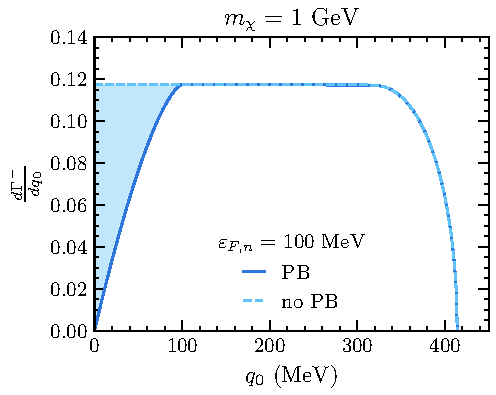
\includegraphics[width=.48\textwidth]{capture_1/diff_intrate_n0_mu_100MeV_mdm1GeV.pdf}
    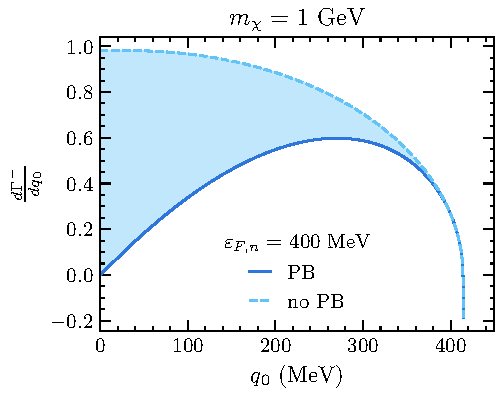
\includegraphics[width=.48\textwidth]{capture_1/diff_intrate_n0_mu_400MeV_mdm1GeV.pdf}\\
    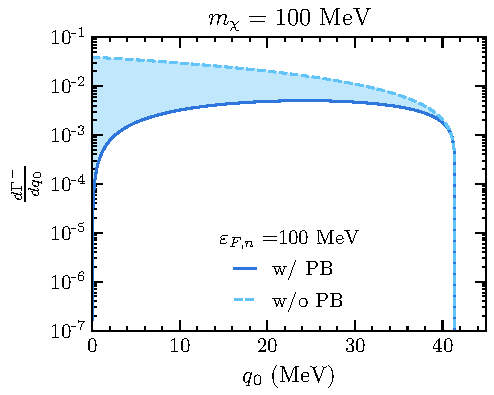
\includegraphics[width=.48\textwidth]{capture_1/diff_intrate_n0_mu_100MeV_mdm100MeV.pdf}
    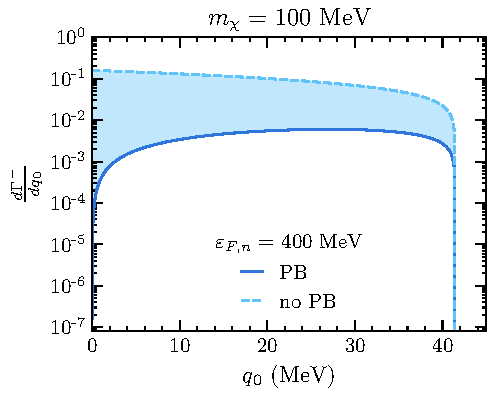
\includegraphics[width=.48\textwidth]{capture_1/diff_intrate_n0_mu_400MeV_mdm100MeV.pdf}\\
    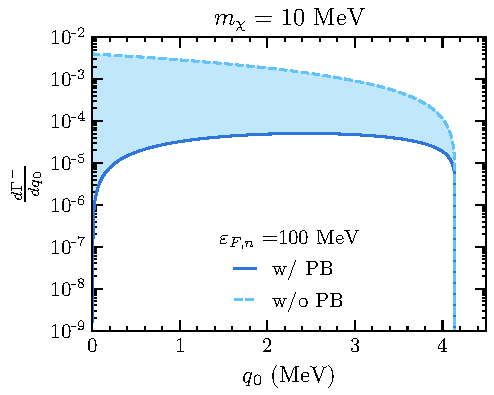
\includegraphics[width=.48\textwidth]{capture_1/diff_intrate_n0_mu_100MeV_mdm10MeV.pdf}
    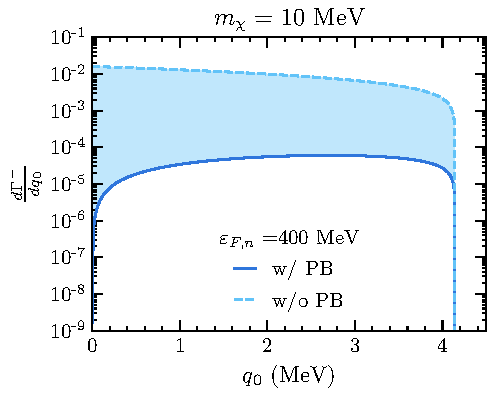
\includegraphics[width=.48\textwidth]{capture_1/diff_intrate_n0_mu_400MeV_mdm10MeV.pdf}
    \caption{Differential interaction rates $\frac{d\Gamma}{dq_0}$  
    as a function of the energy loss $q_0$ for different values of $m_\chi$ and $\kinFn$, constant cross-section and $B=0.5$. Blue lines refer to the result that includes Pauli blocking, while the light blue dashed lines refer to the result without PB. Left column:  $\kinFn=100\MeV$, right column: $\kinFn=400\MeV$. Top: $m_\chi=1\GeV$, middle: $m_\chi=100\MeV$, bottom: $m_\chi=10\MeV$.  }
    \label{ch3:fig:gammaNPBmu}
\end{figure}
%%%%%%%%%%%%%%%%%%%%%%%%%%%%%%%%%%%%%%%%%




To assess the impact of PB on the DM differential interaction rate, in Fig.~\ref{ch3:fig:gammaNPBmu} we compare the rate 
with (blue solid lines) and without (light blue dashed lines) Pauli blocking, for $B=0.5$ and constant DM-neutron cross-section. When Pauli blocking can be neglected, the interaction rate is obtained straightforwardly from Eq.~\ref{ch3:eq:scattrate} by stripping away the $(1 - \fFD(\Ei'))$ factor. 
The difference between the computations is shaded in light blue. In the top left panel, we see that the rate begins to be suppressed from PB at $q_0 \sim \kinFi = 100\MeV$ for a 1~GeV DM.
% we can see how the differential rate changes by switching Pauli blocking on or off, for $\kinFn=100\MeV$.
%  The rate calculated without PB is flat for $q_0\lesssim 200\MeV$, while when Pauli suppression is active it undergoes a smooth transition towards $0$ for $q_0<\kinFn$. 
In the top right plot, we increase the neutron chemical potential from $\kinFn=100\MeV$ to $\kinFn=400\MeV$. Given that in this case $\qomax \sim 0.4 m_\chi \sim 400\MeV$, almost the whole energy range is affected by PB. The higher $\kinFn$ changes the spectra (both with and without PB) such that the unsuppressed rate is no longer flat at low $q_0$. The PB suppressed rate reaches a maximum at values of $q_0$ slightly below $\qomax$, and then decreases towards $0$ at lower $q_0$.
In the middle panels, $m_\chi=100\MeV$, and $\qomax\sim40\MeV\ll\kinFn$. In this case, it is evident that PB affects the spectrum over the full $q_0=\qomax$ range. In the bottom row, we set $m_\chi=10\MeV$. As expected, for lighter DM,  the effects of PB are even more pronounced.



To understand how the effect of PB varies throughout the star, we can analyse the radial profiles of the capture rates $dC/dr$.
In Fig.~\ref{ch3:fig:diffcap} we plot the differential capture rate as a function of the NS radius, with and without Pauli blocking. We see that Pauli blocking is most significant at low DM mass, below about 1~GeV, and becomes insignificant for higher masses. Pauli blocking has a larger impact on the differential capture rate deeper into the NS interior and has a negligible effect at the surface. This is particularly apparent in the top left panel of Fig.~\ref{ch3:fig:diffcap}. This is because the chemical potential is higher in the NS interior than it is near the crust, as seen in the radial $\kinFi$ profile in the bottom left panel of Fig.~\ref{ch2:fig:BSk_profiles}.

%%%%%%%%%%%%%%%%%%%%%%%%%%%%%%%%%%%%%%%%%
\begin{figure}
    \centering
    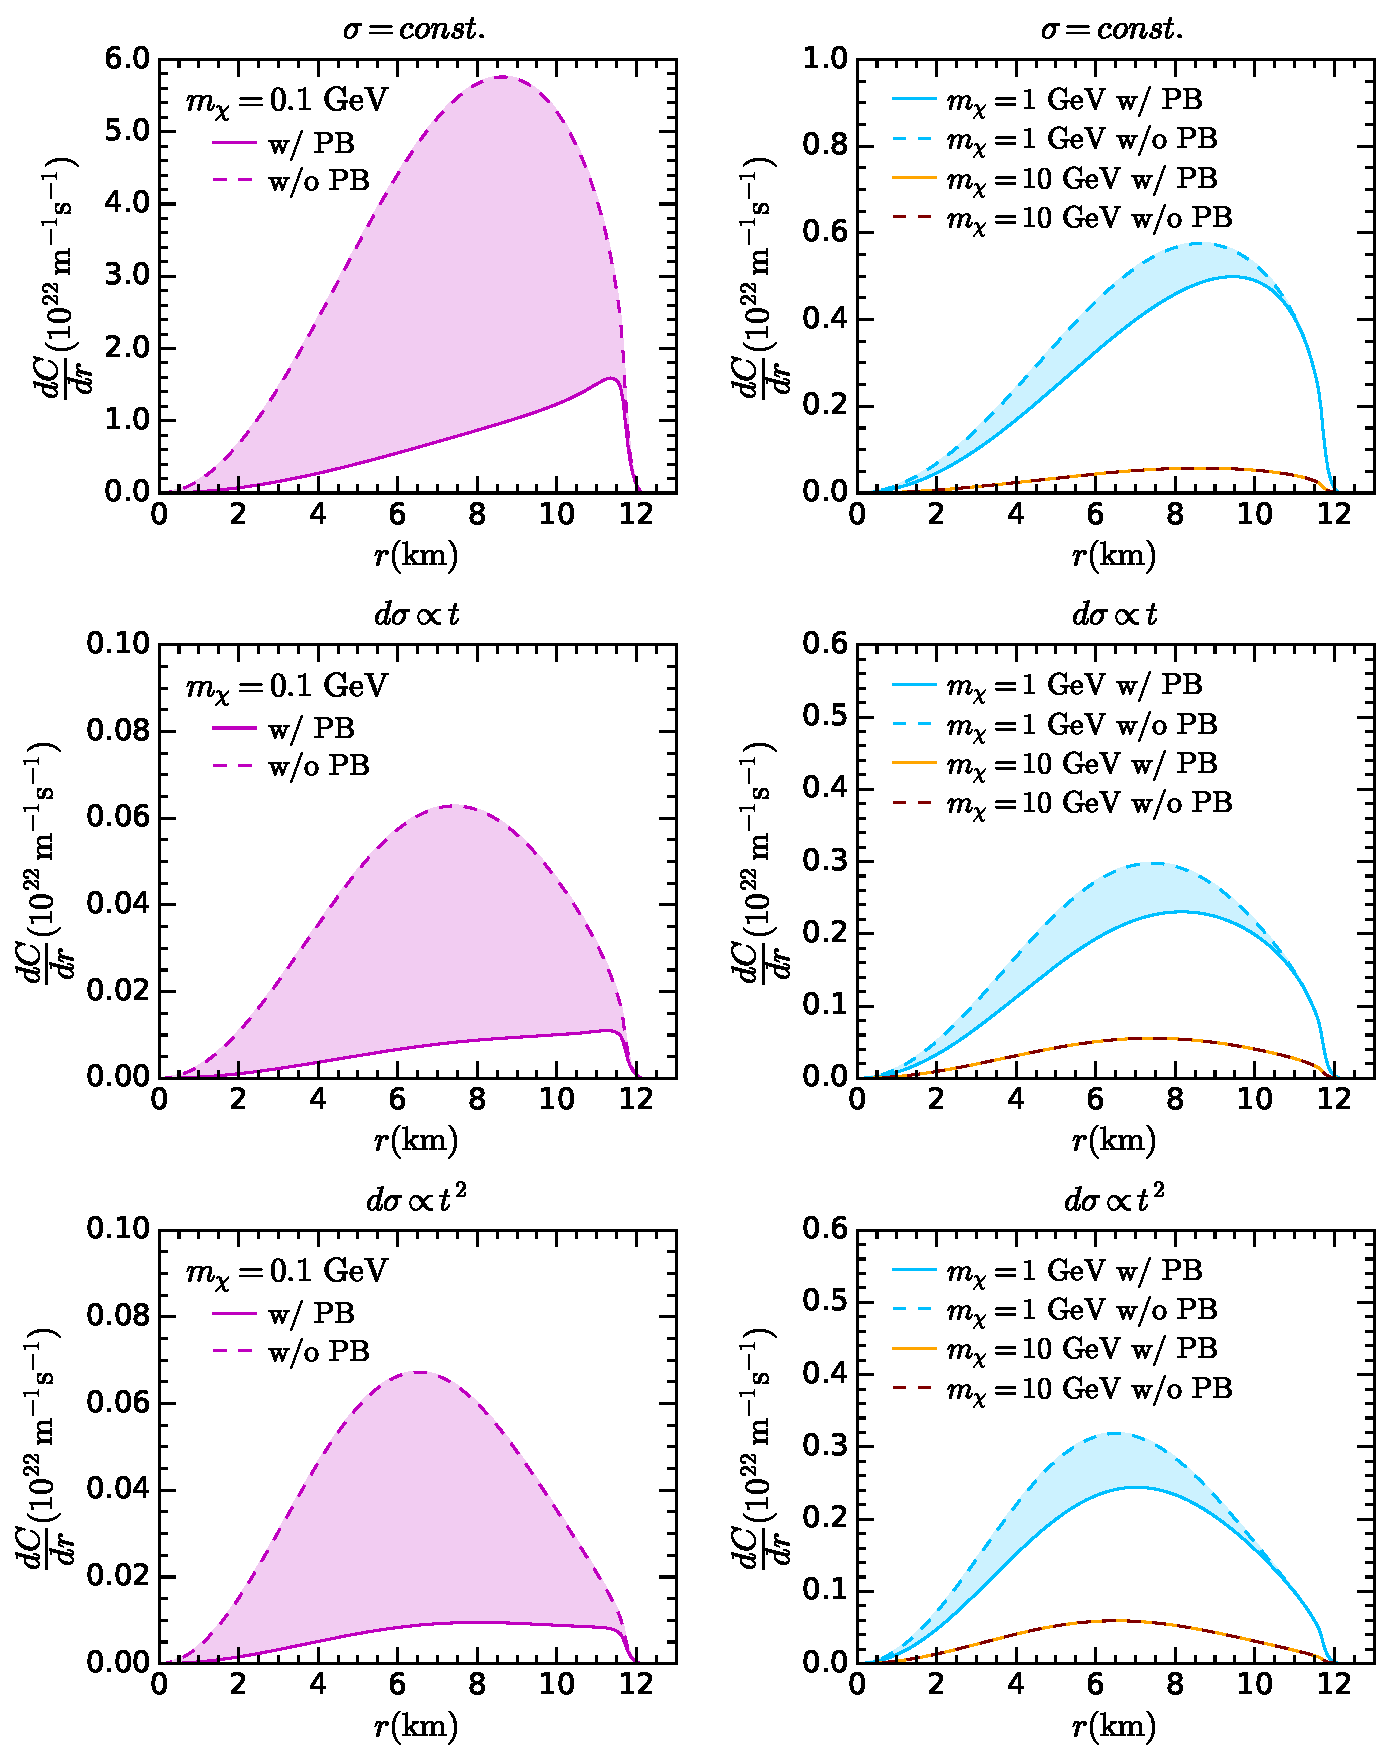
\includegraphics[width=.85\textwidth]{capture_1/diff_cap_rate.pdf}        
    \caption{Differential capture rate as a function of the NS radius $r$, with (solid) and without (dashed) Pauli blocking, for the EoS benchmark BSk24-2. Top: constant cross-section, center: $d\sigma\propto t$, bottom: $d\sigma\propto t^2$.}
    \label{ch3:fig:diffcap}
\end{figure}
%%%%%%%%%%%%%%%%%%%%%%%%%%%%%%%%%%%%%%%%%

%%%%%%%%%%%%%%%%%%%%%%%%%%%%%%%%%%%%%%%%%
%%%%%%%%%%%%%%%%%%%%%%%%%%%%%%%%%%%%%%%%%
%%%%%%%%%%%%%%%%%%%%%%%%%%%%%%%%%%%%%%%%%
\section{Capture in the Low, Intermediate and High Mass Regimes}
\label{ch3:sec:capture_analysis}
%%%%%%%%%%%%%%%%%%%%%%%%%%%%%%%%%%%%%%%%%
%%%%%%%%%%%%%%%%%%%%%%%%%%%%%%%%%%%%%%%%%
%%%%%%%%%%%%%%%%%%%%%%%%%%%%%%%%%%%%%%%%%

Having assembled all the required machinery, we are ready to explore the properties of the capture rate in the three mass regimes outlined in Eq.~\ref{ch3:eq:sigmath}.  Given the computational load required to evaluate Eq.~\ref{ch3:eq:cap_rel_full_1} in general, we aim to provide approximations that are numerically more efficient where possible. We also discuss the high DM mass regime where multiple scatterings are required for capture, and how this is affected by Pauli blocking. 


%%%%%%%%%%%%%%%%%%%%%%%%%%%%%%%%%%%%%%%%%
%%%%%%%%%%%%%%%%%%%%%%%%%%%%%%%%%%%%%%%%%
\subsection{Low and intermediate DM mass range}
\label{ch3:sec:captureintermediate}
%%%%%%%%%%%%%%%%%%%%%%%%%%%%%%%%%%%%%%%%%
%%%%%%%%%%%%%%%%%%%%%%%%%%%%%%%%%%%%%%%%%


In sections~\ref{ch3:sec:captrue_new_full} and \ref{ch3:sec:diff_int_rate}, we have derived general expressions to numerically calculate the DM capture and interaction rates,  
Eqs.~\ref{ch3:eq:cap_rel_full_1} and \ref{ch3:eq:int_rate_capture_full} respectively.   
Using these expressions, we can write 
the complete expression for the capture rate as a function of the differential DM-neutron cross-section 
\begin{equation}
    \begin{split}
        C = \frac{2\rho_\chi}{\pi \vstar m_\chi^2} {\rm Erf}\left(\sqrt{\frac{3}{2}}\frac{\vstar}{v_d}\right)\int_0^{\Rstar}  dr  \frac{r^2\zeta(r)}{\sqrt{B(r)}} &\int dt d\Ei ds \frac{d\sigma}{d\cos\thetacm}\frac{\Ei s}{\beta(s)\gamma(s)}\\
        &\times \fFD(\Ei,r)(1-\fFD(\Ei',r)), 
    \end{split}
\label{ch3:eq:capturefinal}
\end{equation}
where the functions $\beta$ and $\gamma$ were given in section~\ref{ch3:subsec:int_rate_degen_rel}. Recall that in the limit $T\rightarrow0$,  $\fFD(\Ei,r)$ and $1-\fFD(\Ei',r)$  reduce to the step functions,  $\Theta(\kinFi(r)-\Ei)$ and  $\Theta(\Ei'-\kinFi(r))$, respectively. 


Exchanging the differential cross-section for the squared matrix allows for easier examination of the operators in Table~\ref{ch1:tab:opers_defn_full}, and so we write the capture rate as
\begin{equation}
    \begin{split}
        C &=  \frac{\rho_\chi}{8\pi^2 \vstar m_\chi^2} {\rm Erf}\left(\sqrt{\frac{3}{2}}\frac{\vstar}{v_d}\right)\int_0^{\Rstar}   dr  \frac{r^2 \zeta(r) }{\sqrt{B(r)}} & \int dt d\Ei ds \frac{|\overline{M}|^2 \Ei}{2s\beta(s)-\gamma^2(s)} \frac{s}{\gamma(s)} \\
        &\times \fFD(\Ei,r)(1-\fFD(\Ei',r)). 
    \end{split}
    \label{ch3:eq:capturefinalM2}
\end{equation}
This expression can be used to numerically calculate the single scatter capture rate of DM in compact objects, in the optically thin regime. In general, this must be used for low-mass DM where PB is in effect.

As discussed in section~\ref{ch3:subsec:PB_cap}, PB eventually becomes negligible for DM with masses $\gtrsim \muFi$. Hence, between this mass and the point where multiple scattering becomes important, PB can be neglected and a simplified capture rate be obtained. For nucleon targets, this range is between $1\GeV\lesssim m_\chi\lesssim 10^6\GeV$, which we call the intermediate mass range.

The resulting simplified capture rate differs slightly depending on whether the matrix element depends only on $t$, or if it has explicit $s$ dependence. We present the full derivations of these results in Appendix~\fixMV{ADD APPENDICIES}
First, for $|\overline{M}|^2=a t^n$, the previous expression can be simplified to 
\begin{gather}
        C \sim C_\mathrm{approx} = \frac{4\pi}{\vstar} \frac{\rho_\chi}{m_\chi}{\rm Erf}\left(\sqrt{\frac{3}{2}}\frac{\vstar}{v_d}\right)\int_0^{\Rstar}  r^2 dr \, n_i(r)  \frac{1-B(r)}{B(r)} \langle\sigma(r)\rangle 
\label{ch3:eq:csimplelargemtext}, \\
\langle\sigma(r)\rangle = \left\langle\int dt \frac{d\sigma}{dt} \right\rangle_s =   \frac{a}{16\pi m_\chi^2 } \frac{1}{n+1}\left(\frac{4(1-B(r))m_\chi^2}{B(r)(1+\mu^2)}\right)^{n}. 
\label{ch3:eq:xsecave}
\end{gather}
For $s$-dependent matrix elements the result is very similar, with the only difference being that the cross-section is not averaged over $s$, and instead $s$ is fixed to a particular value as detailed in Appendix~\fixMV{ADD APPENDIX}. Writing the matrix element as $\Msq \propto \bar{g}(s)t^n$, for with $g$ some function of $s$, we arrive at the result
\begin{gather}
    C \sim C_{\mathrm{approx}, s} = \frac{4\pi}{\vstar} \frac{\rho_\chi}{m_\chi}{\rm Erf}\left(\sqrt{\frac{3}{2}}\frac{\vstar}{v_d}\right)\int_0^{\Rstar}  r^2 dr \, n_i(r)  \frac{1-B(r)}{B(r)} \sigma(r)
\label{ch3:eq:csimplelargemtext_sdep}, \\
\begin{split}
    \sigma(r) = \int dt \frac{d\sigma}{dt} & =   \frac{1}{16\pi \left(\mi^2 \mchi^2 + 2\mi \mchi/\sqrt{B(r)}\right)}\frac{\bar{g}(s_0)}{(n+1)}\\
    &\hspace{6em}\times\left[\frac{4(1 - B(r)) \mchi^2}{B(r)(1 + \mu^2) + 2\sqrt{B(r)}\mu}\right]^n,
\label{ch3:eq:xsecave_sdep}
\end{split}\\
s_0 = \mi^2 + \mchi^2 + 2\frac{\Ei\mchi}{\sqrt{B(r)}}.
\end{gather}
As with the differential interaction rates, it is the $t$-dependence of the matrix elements that dictate the key features of the capture rate.

%%%%%%%%%%%%%%%%%%%%%%%%%%%%%%%%%%%%%%%
\begin{figure}
    \centering
    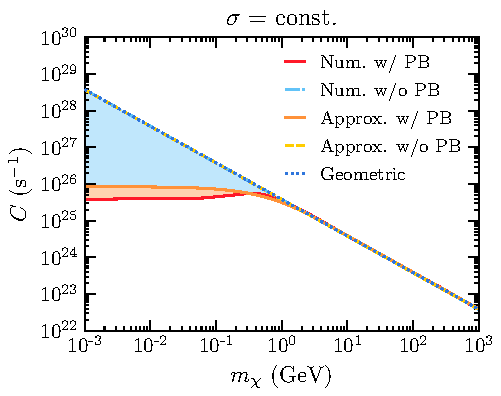
\includegraphics[width=.48\textwidth]{capture_1/capture_rate_n0.pdf}
    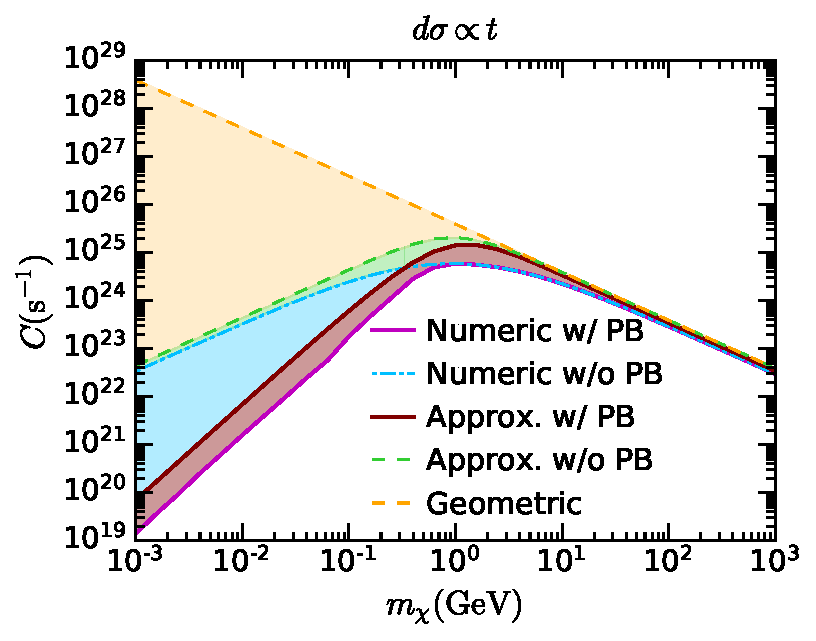
\includegraphics[width=.48\textwidth]{capture_1/capture_rate_n1.pdf}\\
    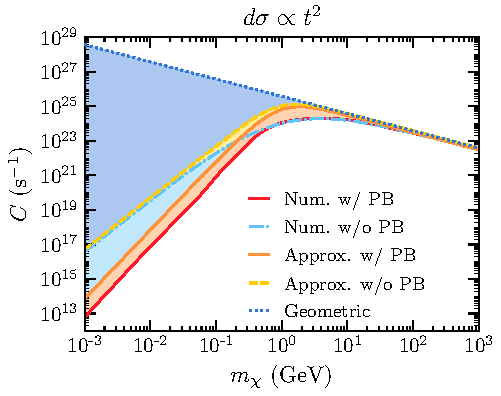
\includegraphics[width=.48\textwidth]{capture_1/capture_rate_n2.pdf}
    \caption{Capture rate as a function of the DM mass with cross-sections normalised to $\sigma=\sigmaref\sim 1.7 \times 10^{-45} \cm^2$, for EoS BSk24-2, calculated with and without Pauli blocking. Top left: constant cross-section. Top right: $d\sigma\propto t$, bottom: $d\sigma\propto t^2$, where $t$ is the Mandelstam variable. All rates are normalised to the geometric limit at large DM mass. }
    \label{ch3:fig:approxc}
\end{figure}
%%%%%%%%%%%%%%%%%%%%%%%%%%%%%%%%%%%%%%%


In Fig.~\ref{ch3:fig:approxc}, we show the capture rate as a function of the DM mass for matrix elements proportional to $t^n$, for $n=0,1,2$ and the NS benchmark model BSk24-2. Numerical results obtained using Eq.~\ref{ch3:eq:capturefinalM2} are shown in solid red; results using the same equation but removing the theta function that enforces Pauli blocking are depicted in light blue; and the approximation for intermediate DM masses, Eq.~\ref{ch3:eq:csimplelargemtext}, in yellow. We show the geometric limit, Eq.~\ref{ch3:eq:capturegeom}, in blue for comparison. 
The capture rates were all normalised to the geometric limit at large DM mass where PB is negligible. 
In the same plots, we also show in brown the result obtained from using a modified version of Eq.~\ref{ch3:eq:csimplelargemtext} to include Pauli blocking.
This is achieved by including the ratio between the differential the interaction rate, $\Gamma^-$, calculated with and without Pauli blocking. This comparison was done in section~\ref{ch3:subsec:PB_cap} for various values of $B$ and $\kinFn$.

From Fig.~\ref{ch3:fig:approxc}, we can see that Eq.~\ref{ch3:eq:csimplelargemtext} is indeed a good approximation to the numerical results obtained without Pauli blocking, and can be safely used for DM masses from a few $\GeV$ up to $m_\chi\sim10^6\GeV$, where multiple scattering becomes relevant. 
On the other hand, for $m_\chi\lesssim 100\MeV$ the brown line is no longer a good approximation to the numerical result with Pauli blocking, as it always overestimates the capture rate by nearly an order of magnitude. Therefore, to accurately account for the effects of PB for low mass DM, the complete expression for the capture rate, Eq.~\ref{ch3:eq:capturefinalM2} must be used and evaluated numerically.

We now compare our full numerical capture rate calculation, Eq.~\ref{ch3:eq:capturefinalM2}, with that of Ref.~\cite{Garani:2018kkd_may_NewAnalysisNeutron}, in Fig.~\ref{ch3:fig:Cratecomp}. The capture rates calculated in Ref.~\cite{Garani:2018kkd_may_NewAnalysisNeutron} correctly include the stellar structure and Pauli blocking, however, they do not account for general relativistic corrections, and the authors only considered the case of a constant cross-section, $\sigma=10^{-45}\cm^2$. Top make the comparison as fair as possible, we have selected NS configurations that match those of Figs.~1 and 14 of Ref.~\cite{Garani:2018kkd_may_NewAnalysisNeutron}, namely their Model A (BSk20-1):  $\Mstar\simeq1.52\Msun$, $\Rstar\simeq11.6\km$ and Model D (BSk21-2): $\Mstar\simeq2.11\Msun$ and $\Rstar\simeq12.0\km$. We denote these new benchmark models as BSk26-1 (left panel of Fig.~\ref{ch3:fig:Cratecomp}) and BSk24-5 (right panel). Note that we were not able to use the BSk20 and BSk21 functionals, since there are no publicly available fits for the chemical potentials and particle abundances for those EoS families. However, as discussed earlier in section \ref{ch2:subsec:NS_EoS}, BSk26 (BSk24) yields configurations that are almost indistinguishable from those obtained with BSk20 (BSk21)~\cite{Perot:2019gwl_Rolesymmetryenergy}.

We can see in the left panel of Fig.~\ref{ch3:fig:Cratecomp} that in the non-Pauli suppressed region, $m_\chi \gtrsim 1\GeV$, our capture rate calculation in the optical thin limit (solid magenta) exceeds that of Ref.~\cite{Garani:2018kkd_may_NewAnalysisNeutron} (dot-dashed blue) by a factor of $\sim 4$. When Pauli blocking is active, our capture rate calculation is about one order of magnitude higher than the classical calculation.  Recall that Ref.~\cite{Garani:2018kkd_may_NewAnalysisNeutron}  accounts for neither gravitational focusing nor relativistic kinematics. 
We also show in dashed light blue the approximation given in Ref.~\cite{McDermott:2010pa_TurningLightsHow}, which accounts for Pauli blocking with a suppression factor that depends on the neutron Fermi momentum $\sim m_\chi v_{esc}/p_{F,n}$ for $m_\chi < m_n$. Though this approximation fails to reproduce the capture rate shape due to Pauli blocking in the DM mass range $[0.1\GeV,10\GeV]$, it underestimates the capture rate by only a factor of 2 when the DM mass is below 0.1 GeV. 
Finally, we compare the geometric limit of Eq.~\ref{ch3:eq:capturegeom}  (solid orange) that incorporates GR effects~\cite{Bell:2018pkk_sep_HeatingNeutronStars} with the non-relativistic expression in Ref.~\cite{Garani:2018kkd_may_NewAnalysisNeutron} (dot-dashed brown). We observe that the former is $\sim 67 \%$ greater than the latter, mostly due to the $1/B(\Rstar)$ GR correction \cite{Goldman:1989nd_WeaklyInteractingMassive,Kouvaris:2007ay_WIMPAnnihilationCooling}. Similar conclusions are obtained when comparing capture rate calculations for Model D of Ref.~\cite{Garani:2018kkd_may_NewAnalysisNeutron} (their Fig.~14) with our approach, as illustrated in the right panel of Fig.~\ref{ch3:fig:Cratecomp}.

%%%%%%%%%%%%%%%%%%%%%%%%%%%%%%%%%%%%%%%%
\begin{figure}
    \centering
    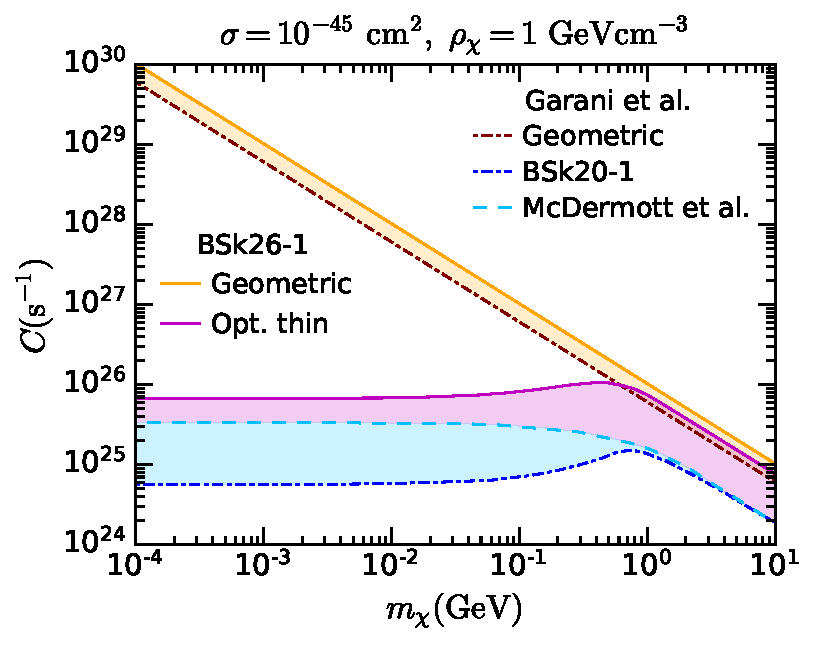
\includegraphics[width=.48\textwidth]{capture_1/capture_rate_n0_comp1.pdf}
    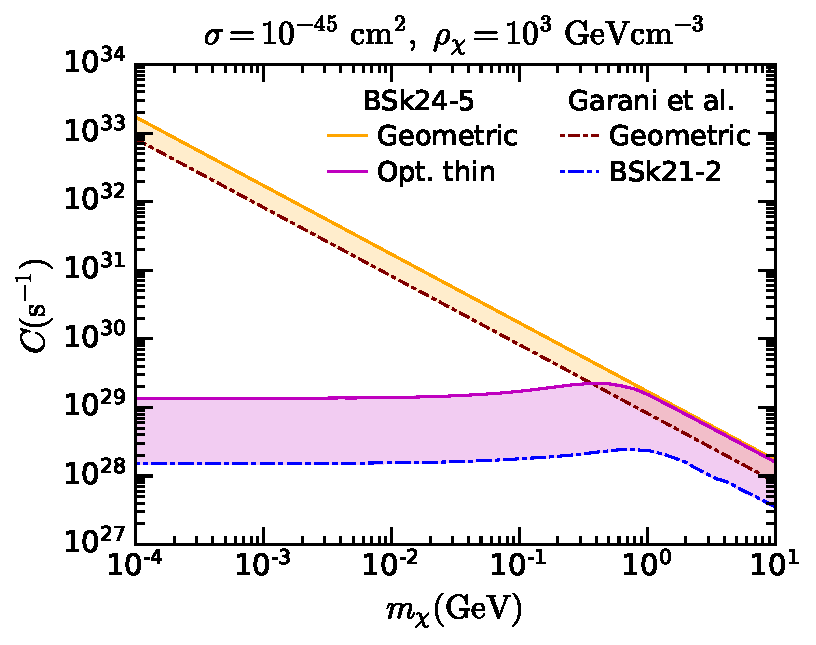
\includegraphics[width=.48\textwidth]{capture_1/capture_rate_n0_comp2.pdf}    
    \caption{Left: Capture rate in the optically thin  (magenta) and geometric (orange) limits as a function of the DM mass for constant cross-section $\sigma=10^{-45}\cm^2$, $\rho_\chi=1\GeV\cm^{-3}$ and BSk26 functional for $\Mstar\simeq1.52\Msun$ and $\Rstar\simeq11.6\km$ denoted as BSk26-1. Capture rate calculations from Ref.~\cite{Garani:2018kkd_may_NewAnalysisNeutron} for a NS configuration with EoS BSk20-1~\cite{Potekhin:2013qqa_Analyticalrepresentationsunified} equivalent to BSk26-1, are shown for comparison. Right: Same as left but for $\rho_\chi=10^3\GeV\cm^{-3}$ and the benchmark model BSk24-5 equivalent to BSk21-2 in Ref.~\cite{Garani:2018kkd_may_NewAnalysisNeutron}: $\Mstar\simeq2.11\Msun$ and $\Rstar\simeq12.0\km$. 
    }
    \label{ch3:fig:Cratecomp}
\end{figure}
%%%%%%%%%%%%%%%%%%%%%%%%%%%%%%%%%%%%%%%%

%%%%%%%%%%%%%%%%%%%%%%%%%%%%%%%%%%%%%%%%
%%%%%%%%%%%%%%%%%%%%%%%%%%%%%%%%%%%%%%%%
\subsection{Large Mass Regime: Multiple Scattering}
\label{sec:largemassandsigma}
%%%%%%%%%%%%%%%%%%%%%%%%%%%%%%%%%%%%%%%%
%%%%%%%%%%%%%%%%%%%%%%%%%%%%%%%%%%%%%%%%


The capture rate expressions obtained in the previous section assume that the cross-section is small enough that the star is in the ``optically thin'' regime, and that a single scatter is sufficient to capture the DM. These assumptions break down if the DM-target cross-section is $\gtrsim\mathcal{O}(\sigmath)$, or if the DM mass exceeds $m_\chi \sim 10^6\GeV$, respectively. 
In this section, we focus on addressing the latter concern as we work in the optically thin regime for the remainder of this work\footnote{The discussion on the effect of the NS opacity in $\sigma\sim \sigmath$ regime can be found in Ref.~\cite{Bell:2020jou_sep_ImprovedTreatmentDark}.}. 
To that end, we now explain how to modify our previous capture rate expressions to account for multiple scattering in a degenerate media\footnote{For a recent discussion on multiple scattering within non-relativistic stars, or with ions in WDs, see Ref.~\cite{Dasgupta:2019juq_Darkmattercapture}.}


In deriving Eq.~\ref{ch3:eq:capturefinal} we had assumed that the DM velocity at infinity, $u_\chi$, can be neglected, such that any interaction where the DM loses energy resulted in its capture. If we instead keep the leading order $u_\chi$ contribution to the total DM energy, the DM energy at infinity is
\begin{equation}
    E^\infty_\chi \sim m_\chi \left(1+\frac{1}{2}u_\chi^2\right), 
\end{equation}
and at a distance $r$ from the star, it gets boosted to
\begin{equation}
    E_\chi(r) = \frac{m_\chi}{\sqrt{B(r)}} \left(1+\frac{1}{2}u_\chi^2\right).
    \label{ch3:eq:Echir}
\end{equation}
Therefore, the amount of energy that the DM must lose to be captured is
\begin{align}
    E_\chi^C(r) & =  \frac{1}{2}u_\chi^2 \frac{m_\chi}{\sqrt{B(r)}}. \\
                & \sim 0.6\GeV \left(\frac{u_\chi}{270\km\s^{-1}}\right)^2 \left(\frac{m_\chi}{10^6\GeV}\right)\left(\frac{0.5}{B(r)}\right)^{1/2}.
\end{align} 
Hence, DM with a mass of $10^6\GeV$ is required to lose 0.6 GeV for it to be captured. This is of the same order as the maximum amount of energy that can be lost in a single scatter as seen in Fig.~\ref{ch3:fig:q0max}. Given that $\qomax$ plates for $\mchi \gg \mi$, it will be highly improbable that DM heavier than $\sim 10^6\GeV$ loses enough energy in a single scatter to be captured. Single scatter capture is still possible as the DM velocity at infinity is not a fixed value, rather it follows by some distribution function. Therefore, the heavy DM could have a velocity close to zero at infinity, significantly reducing the amount of energy it needs to lose.

To account for this effect, we assume that the DM particles have a speed $u_\chi\ll 1$ at infinity that follows a Maxwell-Boltzmann (MB) distribution, Eq.~\ref{ch3:eq:MB}. 
We can then define the probability density function (PDF) of the energy lost by the DM using the differential interaction rate through
\begin{equation}
\xi(q_0,E_\chi,\kinFi) = \frac{1}{\Gamma(E_\chi)}\frac{d\Gamma}{dq_0}(q_0,E_\chi,\kinFi),\label{ch3:eq:normintrate}
\end{equation}
where $\frac{d\Gamma}{dq_0}$ is the DM differential interaction rate, calculated in Appendix~\ref{ch3:sec:diff_int_rate}. 
The function $\xi$ is defined for any $q_0\ge 0$, however, kinematics dicatates that the function is non-zero only for $q_0\le\qomax$. Additionally, note that $\xi$ depends on $B(r)$ through the ratio $E_\chi/m_\chi$, and for brevity we will simply write $\xi(q_0)$.



%%%%%%%%%%%%%%%%%%%%%%%%%%%%%%%%%%
\begin{figure}[t]
    \centering
    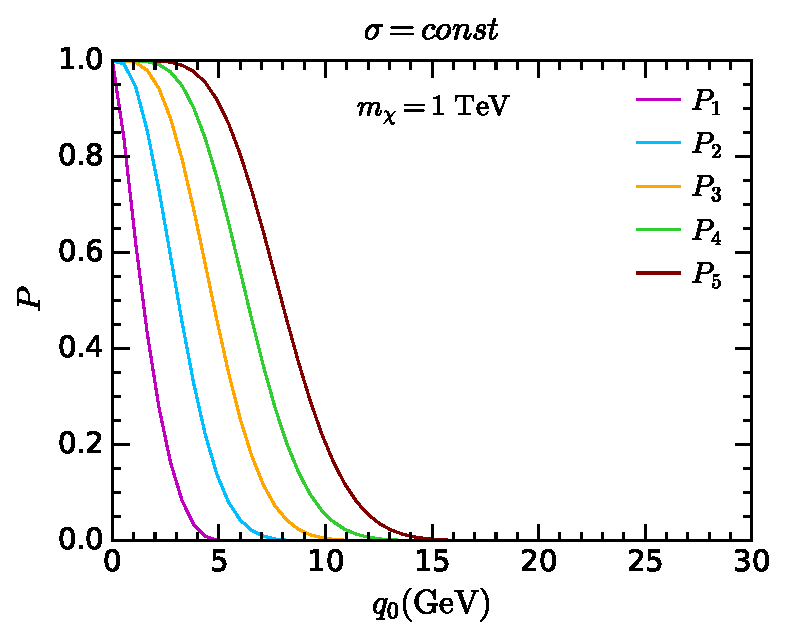
\includegraphics[width=.48\textwidth]{capture_1/probs_n0.pdf}
    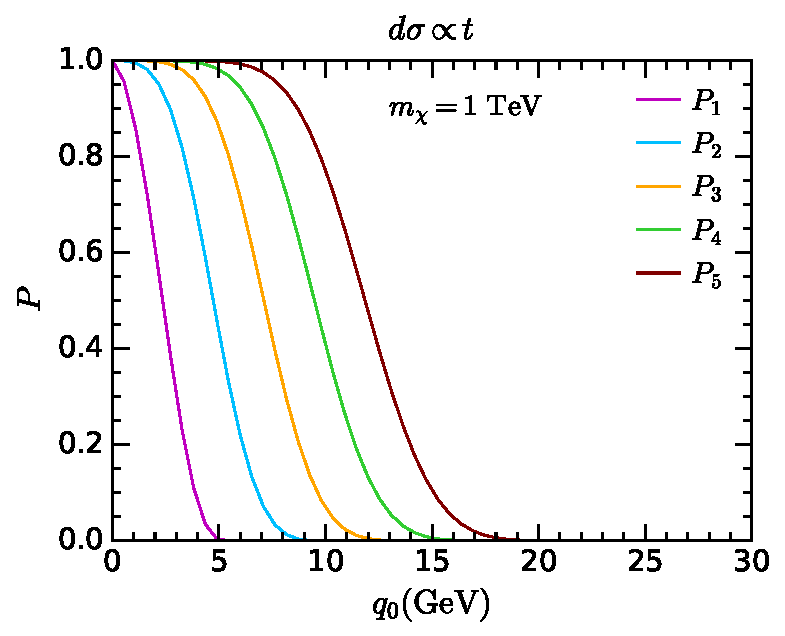
\includegraphics[width=.48\textwidth]{capture_1/probs_n1.pdf}\\
    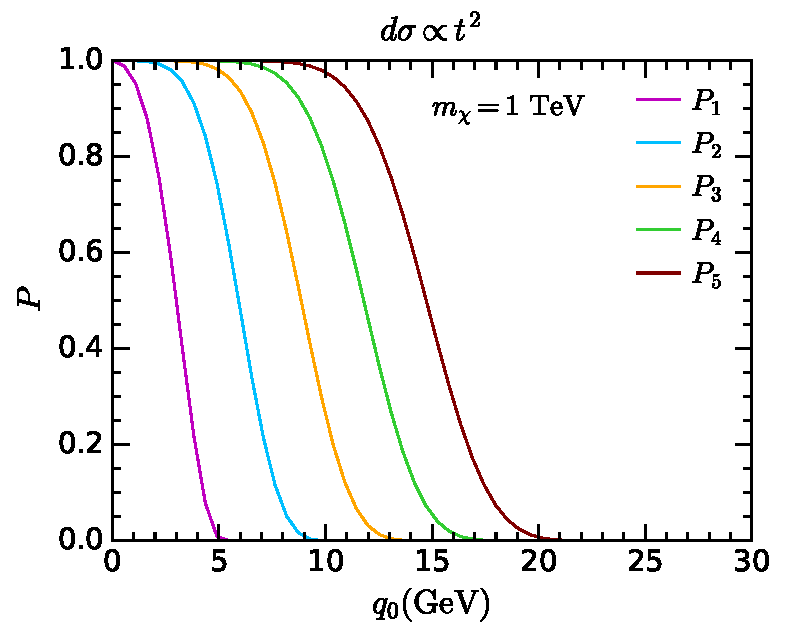
\includegraphics[width=.48\textwidth]{capture_1/probs_n2.pdf}
    \caption{Probabilities to lose at least an amount of energy $\delta q_0$  after $1,...,5$ scatterings,  $P_1,...,P_5$, as a function of the energy loss $q_0$,  assuming $B=0.5$ and $\kinFn=400\MeV$. Results are shown for different dependence on the cross-section on the Mandelstam variable $t$: constant DM-neutron cross-section (top left), $d\sigma\propto t$ (top right) and $d\sigma\propto t^2$ (bottom). }
    \label{ch3:fig:pn}
\end{figure}
%%%%%%%%%%%%%%%%%%%%%%%%%%%%%%%%%%%


We can define the probability of losing at least an amount of energy $q_0 = \delta q_0$ in a single collision as
\begin{equation}
    P_1(\delta q_0) = \int_{\delta q_0}^\infty dx \xi(x).
    \label{ch3:eq:P1}
\end{equation}
The probability of losing at least the same amount of energy after 2 collisions will then be
\begin{align}
 P_2(\delta q_0) &= \int_{\delta q_0}^\infty dy \int_0^\infty dx\;\xi(x) \xi(y-x)\\
    & =  P_1(\delta q_0) + \int_{\delta q_0}^\infty dy \int_0^y dx\; \xi(x)\xi(y-x)\\
    & = P_1(\delta q_0) + \int_0^{\delta q_0} dz \;P_1(\delta q_0-z)\xi(z).
\end{align}
From this, we obtain the following recursive relation for the probabilities, $P_N$, of losing at least $q_0 = \delta q_0$ in $N$ scatters,
\begin{equation}
 P_{N+1}(\delta q_0) = P_N(\delta q_0) + \int_0^{\delta q_0} dz P_N(\delta q_0-z)\xi(z).\label{ch3:eq:pnrecurrent}
\end{equation} 
In Fig.~\ref{ch3:fig:pn} we show how the probability functions $P_1,...,P_5$ changes based on the $t$ dependence of the differential cross-section. We show results for $\sigma=$const. (top left), $d\sigma\propto t$ (top right) and $d\sigma\propto t^2$ (bottom), for fixed values of $B=0.5$, $\kinFn=400\MeV$.

%%%%%%%%%%%%%%%%%%%%%%%%%%%%%%
\begin{figure}
    \centering
    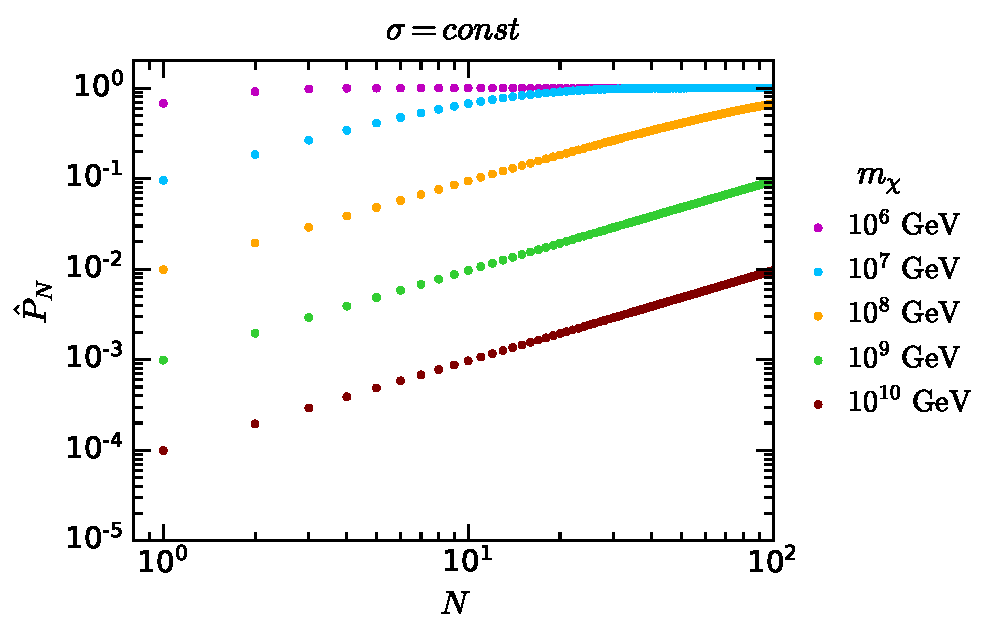
\includegraphics[width=.6\textwidth]{capture_1/cumprobN_n0.pdf}
    \caption{Cumulative probability $\hat{P}_N$ for $B=0.5$,  $\kinFn=400\MeV$ and for $\sigma = \mathrm{const.}$ as a function of the number of scatterings $N$ for several DM masses.}
    \label{ch3:fig:pnofn}
\end{figure}
%%%%%%%%%%%%%%%%%%%%%%%%%%%%%%

To connect this back to the capture probability, we define the probability for a DM particle to be captured after exactly $N$ interactions, $c_N$, to be $P_N(E^C_\chi) - P_{N-1}(E^C_\chi)$ averaged over the MB distribution of the initial velocity,
\begin{equation}
    \begin{split}
        c_N(r) &= \frac{1}{\int_0^\infty \frac{\fMB(u_\chi)}{u_\chi}du_\chi}\int_0^\infty \frac{\fMB(u_\chi)}{u_\chi}du_\chi \left[P_N\left(\frac{1}{2}\frac{m_\chi u_\chi^2}{\sqrt{B(r)}}\right)\right.\\
        &\hspace{18em}\left. -P_{N-1}\left(\frac{1}{2}\frac{m_\chi u_\chi^2}{\sqrt{B(r)}}\right)\right], 
    \end{split}
\end{equation}
where $c_N$ depends on $r$ through the dependence of $P_N$  on $B(r)$ and $\kinFn(r)$. Note that although our results will assume a Maxwell-Boltzmann velocity distribution, it is straightforward to generalise the results to any other DM velocity distribution. The cumulative probability $\hat{P}_N$ that a DM particle is captured after $N$ interactions with a total energy loss  $\delta q_0=E_\chi^C$ is then
\begin{equation}
\hat{P}_N(r) = \sum_{i=1}^N c_i = \frac{1}{\int_0^\infty \frac{\fMB(u_\chi)}{u_\chi}du_\chi}\int_0^\infty \frac{\fMB(u_\chi)}{u_\chi}du_\chi P_N\left(\frac{1}{2}\frac{m_\chi}{\sqrt{B(r)}} u_\chi^2\right).
\end{equation}
%
The resulting cumulative probability is shown as a function of the number of scatterings $N$ in Fig.~\ref{ch3:fig:pnofn}, for constant cross-section and several DM masses. 

The cumulative probability $\hat{P}_N$ for the above values of $B,\kinFn$ is well approximated by the function\footnote{Further discussion of the multi-scattering regime, and justification of this fitting function, can be found in Appendix~C of Ref.~\cite{Bell:2020jou_sep_ImprovedTreatmentDark}.}
\begin{equation}
\hat{P}_N \sim  1-e^{-\frac{N \mstar}{m_\chi}}.\label{ch3:eq:pncum}
\end{equation}
In particular, the probability that the DM is captured in a single scatter is 
\begin{equation}
c_1=\hat{P}_1 \sim  1-e^{-\frac{\mstar}{m_\chi}}.
\label{ch3:eq:c1}
\end{equation}
From this, we see that $c_1$ will begin to significantly fall below unity for $\mchi \gtrsim \mstar$, and hence multiple scattering will only significantly reduce the capture rate for DM masses above $\mstar$. 

To give an idea for how large the value of $\mstar$ will be, for neutron targets and the values $B=0.5$ and $\kinFn=400$~MeV, we find
\begin{align}
m^{*} &=1.08 \times 10^6 \GeV,\quad |\overline{M}|^2\propto t^0,\\
m^{*} &=1.62 \times 10^6 \GeV,\quad |\overline{M}|^2\propto t^1,\\
m^{*} &=2.01 \times 10^6 \GeV,\quad |\overline{M}|^2\propto t^2.
\end{align}
We illustrate how $m^*_n$ varies with $B$ and $\kinFn$ in Fig.~\ref{ch3:fig:mstarbmu}. 

%%%%%%%%%%%%%%%%%%%%%%%%%%%%%%
\begin{figure}[t!bp]
    \centering
    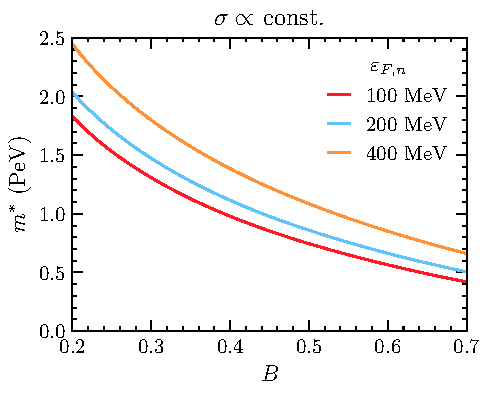
\includegraphics[width=.48\textwidth]{capture_1/mstar_B_n0.pdf}
    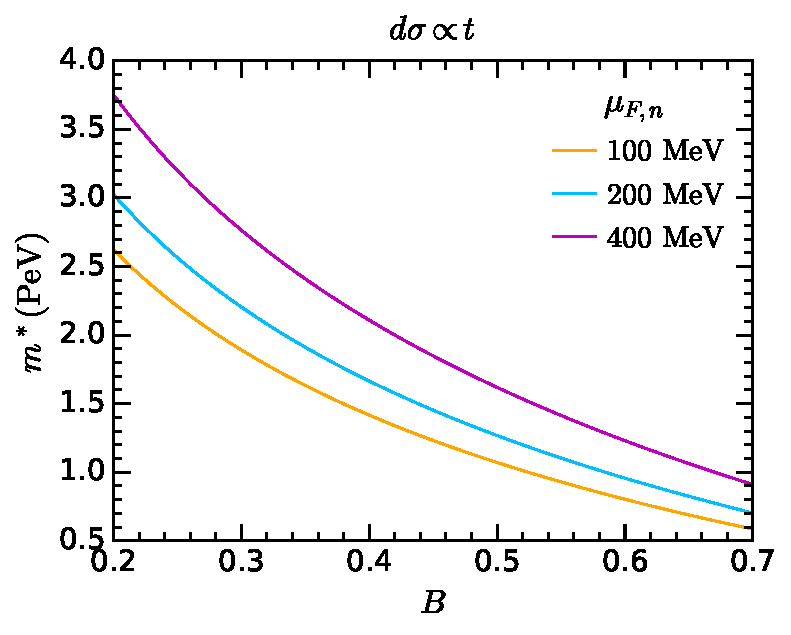
\includegraphics[width=.48\textwidth]{capture_1/mstar_B_n1.pdf}    
    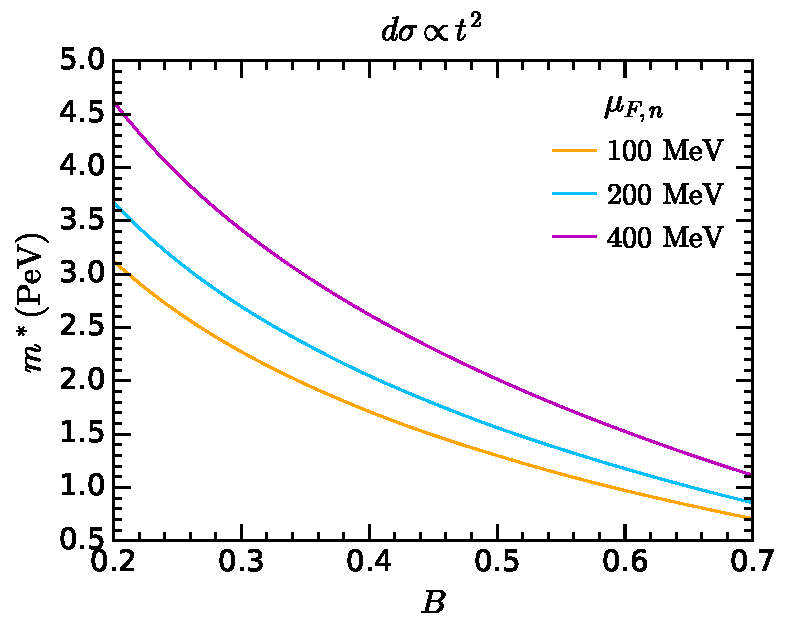
\includegraphics[width=.48\textwidth]{capture_1/mstar_B_n2.pdf}      
    \caption{Value of $m^*_n$ as a function of $B$ for different values of $\kinFn$, $\sigma=const.$ (top left), $d\sigma\propto t$ (top right) and $d\sigma\propto t^2$ (bottom).}
    \label{ch3:fig:mstarbmu}
\end{figure}
%%%%%%%%%%%%%%%%%%%%%%%%%%%%%%

When the cross-section is small, $\sigma\ll\sigmath$, such that we are in the optically thin regime, if the DM does not get captured in its initial scatter, then it will leave the star without interacting again. To account for this, the factor of $c_1$ should be included in the capture rate calculation, Eq.~\ref{ch3:eq:cap_rel_full_1}. However, as we have jsut seen, $c_1\ll1$ only for $\mchi\gtrsim\mstar$, which will always be significantly larger than the target mass and chemical potential. Therefore, multiple scattering is only important in the regime where PB is negligible, and so a suitable approximation for the capture rate in this regime is
\begin{equation}
    C_\mathrm{approx}^* = \frac{4\pi}{\vstar}\frac{\rho_\chi}{m_\chi}{\rm Erf}\left(\sqrt{\frac{3}{2}}\frac{\vstar}{v_d}\right)  \int  r^2 dr  \frac{\sqrt{1-B(r)}}{B(r)}\Omega^{-}(r) c_1(r).
    \label{ch3:eq:capturesimplelargem}
\end{equation}
    
% %%%%%%%%%%%%%%%%%%%%%%%%%%%%%%%%%%%%%
% %%%%%%%%%%%%%%%%%%%%%%%%%%%%%%%%%%%%%
\section{Results}
\label{ch3:sec:results}
% %%%%%%%%%%%%%%%%%%%%%%%%%%%%%%%%%%%%%
% %%%%%%%%%%%%%%%%%%%%%%%%%%%%%%%%%%%%%


In this section, we present our results for the capture rate of fermionic DM scattering from neutrons within a NS in the zero temperature approximation. We calculate the capture rate only for scalar/pseudoscalar-scalar/pseudoscalar interactions between DM and neutrons, i.e. effective operators D1-D4 in Table~\ref{ch1:tab:opers_defn_full}, whose differential cross-sections depend only on the Mandelstam variable $t$ and not on $s$. 
We assume realistic radial profiles for the neutron number density, chemical potential, and relativistic corrections encoded in $B(r)$ as explained in section~\ref{ch2:subsec:NS_EoS} for the configurations of the EoS BSk24 in Table~\ref{ch2:tab:BSk_configs}. 

\fixMV{Fix to include the s-dep changes made}
Most of our results apply generally to other operators or to other targets (with the mass ranges adjusted appropriately).  Specifically, Eqs.~\ref{eq:captureclsimplrel},~\ref{eq:omegampaulitext}, which are to be evaluated numerically, are applicable to all operators and targets, and work until multiple scattering becomes relevant, when $m_\chi\gtrsim \qomax/v_{\star}^2$.
The optical factor of Eq.~\ref{eq:optfactor} for the intermediate mass range is also applicable to all operators and targets. The optical factor of Eq.~\ref{eq:optfactorlargem} and the value of $m^*$, which are used to include multiple scattering effects in the large mass range, $m_\chi\gtrsim \qomax/v_{\star}^2$, can be easily computed for operators D1-D4 (or any other operator that depends only on $t$) for all targets. For other operators it can be used only by numerically solving the shape of the differential rate, a task that may be computationally intensive to achieve with high precision.
Our approximated formulas, Eqs.~\ref{eq:csimplelargemtext},~\ref{eq:capturesimplelargem} and \ref{eq:captureopticaldepth} have been checked to be accurate only for nucleon targets, but can be applied to any operator (for $s$-dependent ones, see Appendix~\ref{sec:capratesimple} on how to remove the $s$ dependence). In any case, one can substitute the relevant factors ($\eta,m^*$) into Eqs.~\ref{eq:captureclsimplrel},~\ref{eq:omegampaulitext} to calculate the capture rate, in the appropriate mass range, for other targets.







In order to estimate the NS EoS impact on the DM capture rate computation,  we numerically calculate it using the exact expression in the optically thin limit, Eq.~\ref{eq:capturefinal}, that properly accounts for gravitational focusing and Pauli blocking but neglects the star opacity.  In this approximation, the capture rate is proportional to the differential DM-neutron cross-section. 
Fig.~\ref{ch3:fig:captureEOS} shows how this rate varies with the NS  EoS  for operators D1-D4 and the EoS configurations given in Table~\ref{tab:eos}, and in turn with the NS mass and radius. 
The value of the cross-section was chosen so that at large DM mass the capture rate is equal to the geometric limit. 
Note that properly including the optical depth factor $\eta$ would have given a lower value of $C$ (see section~\ref{sec:largemassandsigma}). It is worth remarking that we  should not use larger values of the cross-section in the optically thin approximation, as this would lead to capture rates exceeding the geometric limit.
Depending on the operator considered, going from the lightest to the heaviest NS can change the capture rate by a minimum of one order of magnitude, such as in the case of operators D1, D2 and D3 (at low DM mass), and up to 2 orders of magnitude, as in the case of operators D2 (only at large DM mass) and D4. 

%%%%%%%%%%%%%%%%%%%%%%%%%%%%%%
\begin{figure}
    \centering
    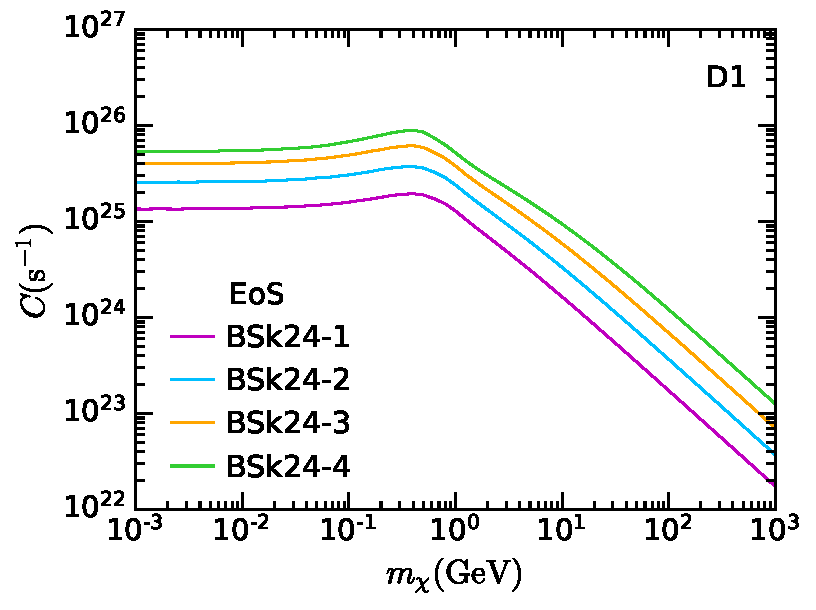
\includegraphics[width=.45\textwidth]{capture_1/capture_rate_numeric_EOS_D1.pdf}
    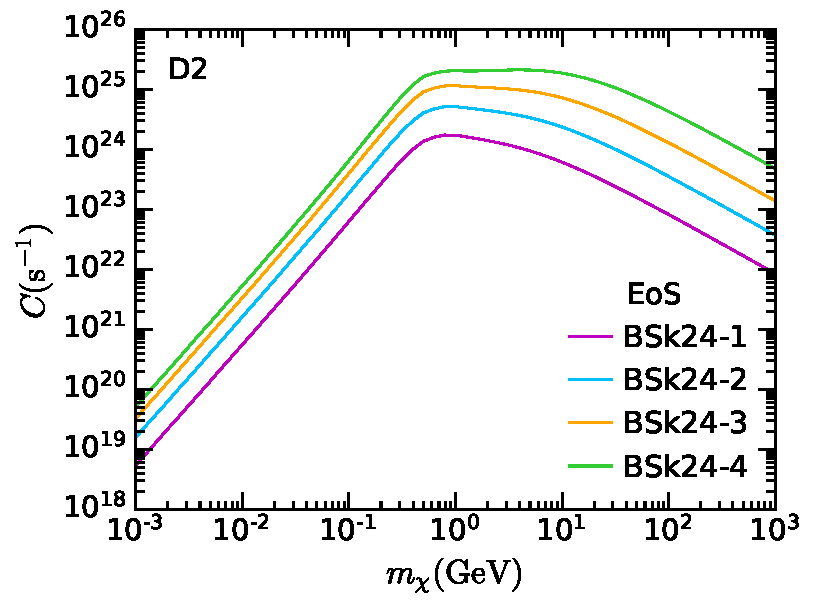
\includegraphics[width=.45\textwidth]{capture_1/capture_rate_numeric_EOS_D2.pdf}\\
    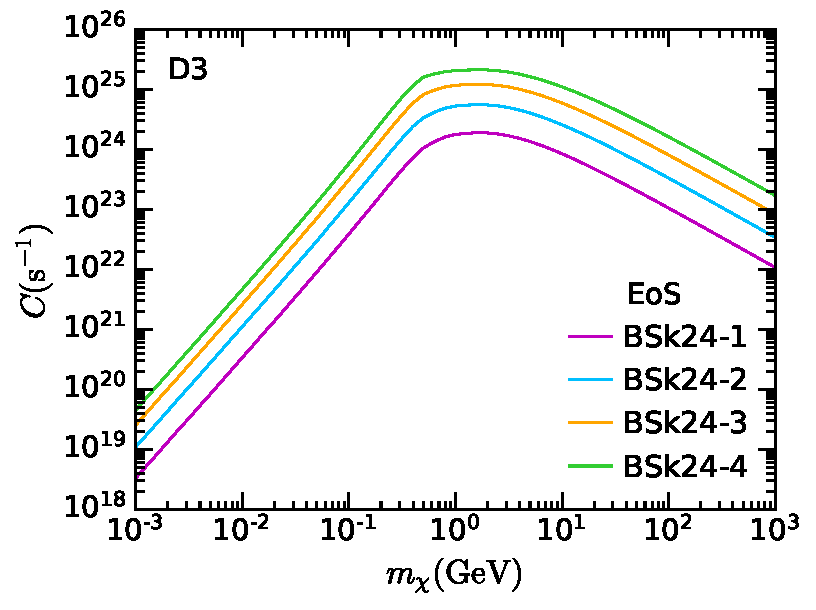
\includegraphics[width=.45\textwidth]{capture_1/capture_rate_numeric_EOS_D3.pdf}
    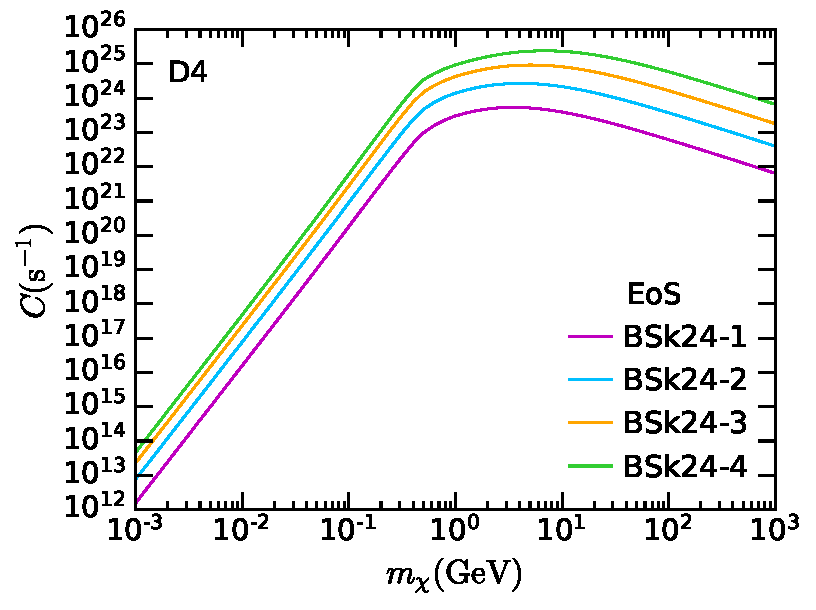
\includegraphics[width=.45\textwidth]{capture_1/capture_rate_numeric_EOS_D4.pdf}
    \caption{Capture rate in the optically thin limit as a function of the DM mass for $\sigma=\sigma_{ref}\sim 1.7 \times 10^{-45} \cm^2$ and the configurations of the EoS BSk24 given in Table~\ref{tab:eos}. Rate calculated using the 4-dimensional integral in Eq.~\ref{eq:capturefinal}, which includes Pauli blocking and neglects the  NS opacity and multiple scattering for the EFT operators D1 (top left), D2 (top right), D3 (bottom left) and D4 (bottom right) in Table~\ref{tab:operatorshe}.}
    \label{ch3:fig:captureEOS}
\end{figure}
%%%%%%%%%%%%%%%%%%%%%%%%%%%%%%




At large DM mass, all operators  show the same scaling with the DM mass. At  $m_\chi\lesssim1\GeV$, a different picture arises as Pauli blocking leads to different suppressions of the capture rate for the different operators. However, we observe that the four operators give very similar results to those of Fig.~\ref{ch3:fig:approxc}, where we analysed the dependence of the capture rate on the momentum transfer $t$.  We note that  operator D1, which contains in its squared matrix element, $|\overline{M}|^2$, a term independent of $t$, gives a result that is very similar to that of $\sigma=const$. Operators D2 and D3, for which $|\overline{M}|^2$ does not include terms independent of $t$, but rather terms proportional to $t$ and $t^2$, yield  very similar results to that of $d\sigma\propto t$. 
Overall, we conclude that the lowest power of the transferred momentum determines the mass scaling of the capture rate at low DM  mass.







%%%%%%%%%%%%%%%%%%%%%%%%%%%%%%
\begin{figure}
    \centering
    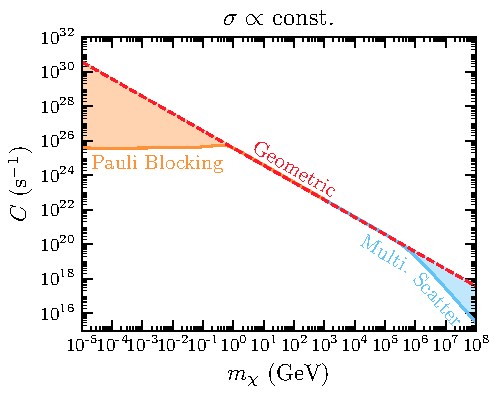
\includegraphics[width=.45\textwidth]{capture_1/capture_rate_n0_fullmassrange.pdf}    
    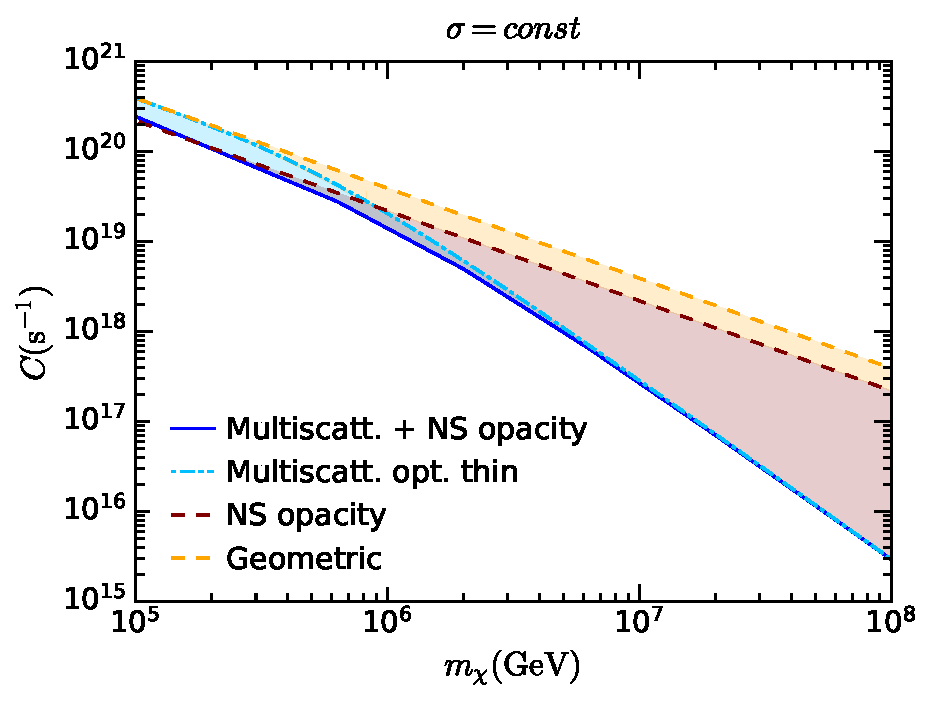
\includegraphics[width=.45\textwidth]{capture_1/capture_rate_n0_largemass.pdf} %\\
    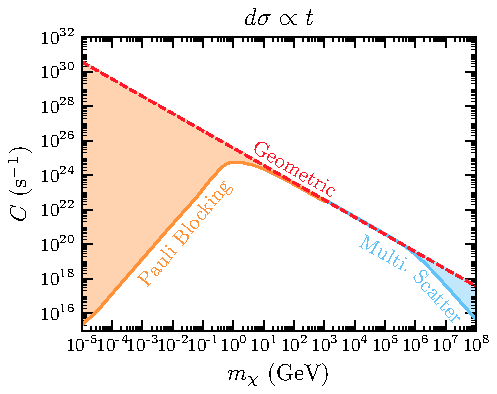
\includegraphics[width=.45\textwidth]{capture_1/capture_rate_n1_fullmassrange.pdf}       
    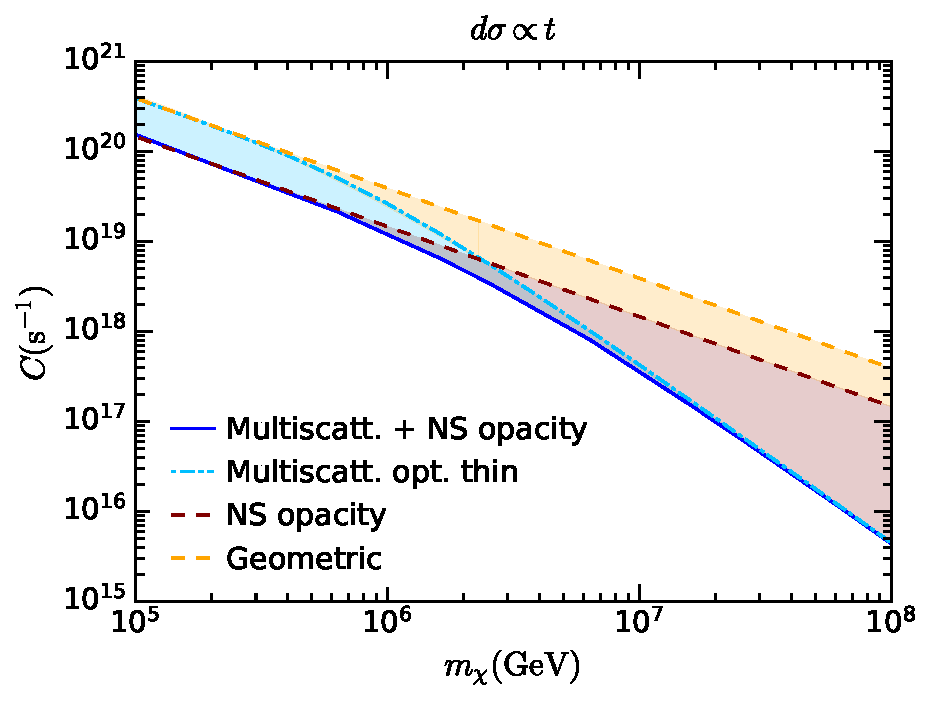
\includegraphics[width=.45\textwidth]{capture_1/capture_rate_n1_largemass.pdf} \\
    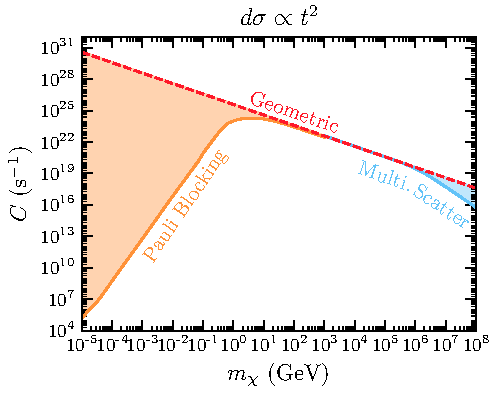
\includegraphics[width=.45\textwidth]{capture_1/capture_rate_n2_fullmassrange.pdf}       
    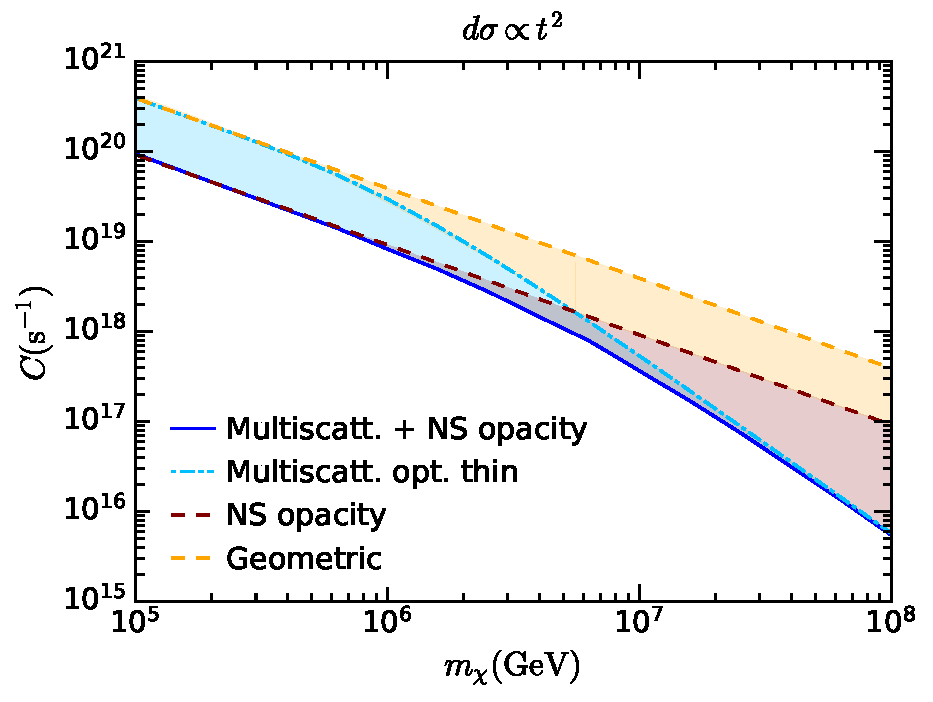
\includegraphics[width=.45\textwidth]{capture_1/capture_rate_n2_largemass.pdf}        
    \caption{Capture rate for constant cross-section (top row), $d\sigma\propto t$ (middle row) and $d\sigma\propto t^2$ (bottom row),  for  $\sigma=\sigma_{ref}\sim 1.7 \times 10^{-45}\cm^2$ and NS EoS configuration BSk24-2. We extend the plot in the top left panel of Fig.~\ref{ch3:fig:approxc} to large DM masses. Left: Full mass range. Right: Same as before but only for large DM mass range. 
    }
    \label{ch3:fig:capturelargemass}
\end{figure}
%%%%%%%%%%%%%%%%%%%%%%%%%%%%%%

In Fig.~\ref{ch3:fig:capturelargemass}, we show the capture rate for a broad DM mass range, spanning 13 orders of magnitude from $m_\chi=10\keV$ to $m_\chi=10^8\GeV$, including all the regimes identified in Table~\ref{tab:caprecap}, for $d\sigma\propto const.$ (first row), $t^1$ (second row) and $t^2$ (third row).
In the left panels, we show the full mass range.  As in previous figures, the magenta line indicates the capture rate calculated in the optically thin limit using the 4-dimensional integration in Eq.~\ref{eq:captureclsimplrel} that accounts for Pauli blocking. 
At large DM masses, Pauli suppression plays no role and the capture rate approaches the geometric limit (dashed orange line). 
We also show in Fig.~\ref{ch3:fig:capturelargemass} three new lines, portraying the effect of the inclusion of the NS optical depth and multiple scattering, which become relevant at $m_\chi\sim10^6\GeV$. 
The difference among these calculations is better shown in the right panels, where only the large DM mass range is considered. The brown dashed line indicates the result that includes the optical depth factor $\eta$ but neglects multiple scattering, obtained using Eq.~\ref{eq:optfactor} in Eq.~\ref{eq:captureopticaldepth}.   
As we can see, for $\sigma=\sigma_{ref}$ this causes a small suppression of the capture rate, when compared to the result where the optical depth factor is ignored (light blue dot dashed line). For larger $\sigma$, neglecting the optical depth would result in a capture rate that exceeds the geometric limit (orange dashed line), while the inclusion of the optical depth factor $\eta$ causes the capture rate to saturate, tending to  $C_{geom}$ for large cross-sections. 
The light blue dot dashed line indicates the capture rate calculated by neglecting the optical depth factor, but including multiple scattering, given by Eq.~\ref{eq:capturesimplelargem}. At $m_\chi\sim 10^5\GeV$ that line matches the geometric limit, due to the chosen value of the cross-section $\sigma=\sigma_{ref}$. On the other hand, at larger DM masses $m_\chi\gtrsim10^6\GeV$, multiple scattering is required to capture DM particles, hence an additional suppression factor of $1/m_\chi$ arises, as given in Eq.~\ref{eq:capturesimplelargem}. Therefore the capture rate becomes increasingly smaller than $C_{geom}$ (orange and brown shaded areas). Finally, the capture rate calculated including both effects is depicted in blue. At $m_\chi\sim10^5\GeV$, we can observe the suppression produced by the optical depth factor $\eta$ (light blue shaded region), while at larger DM masses the proper additional suppression $1/m_\chi$ emerges. 

Comparing the plots for different $t^n$ dependence, we can see that increasing the power of $n$ has a small effect on the mass scale where the various suppressions become relevant. For example, comparing the blue and light blue lines, which both include multiple scattering effects, we see that the change of slope moves further to the right for larger $n$. This is a consequence of the fact that larger powers of $n$ result in larger energy transfer (see, for example, Fig.~\ref{ch3:fig:diffgamma}) and therefore a larger capture probability $c_1$ and larger $m^*$.
However, the qualitative behaviour is the same for all choices of $d\sigma$: the suppression of the capture rate is primarily due to Pauli blocking at low mass, opacity effects in the $1$--$10^6$~GeV mass range, and multiscattering effects (i.e. a low capture probability) at the largest masses.


% %%%%%%%%%%%%%%%%%%%%%%%%%%%%%%%%%%%%%
% %%%%%%%%%%%%%%%%%%%%%%%%%%%%%%%%%%%%%
% %%%%%%%%%%%%%%%%%%%%%%%%%%%%%%%%%%%%%
% \section{White Dwarfs: Electron Targets}
% %%%%%%%%%%%%%%%%%%%%%%%%%%%%%%%%%%%%%
% %%%%%%%%%%%%%%%%%%%%%%%%%%%%%%%%%%%%%
% %%%%%%%%%%%%%%%%%%%%%%%%%%%%%%%%%%%%%

% %%%%%%%%%%%%%%%%%%%%%%%%%%%%%%%%%%%%%
% %%%%%%%%%%%%%%%%%%%%%%%%%%%%%%%%%%%%%
% %%%%%%%%%%%%%%%%%%%%%%%%%%%%%%%%%%%%%
% \section{Neutron Stars: Leptoinc Targets}
% %%%%%%%%%%%%%%%%%%%%%%%%%%%%%%%%%%%%%
% %%%%%%%%%%%%%%%%%%%%%%%%%%%%%%%%%%%%%
% %%%%%%%%%%%%%%%%%%%%%%%%%%%%%%%%%%%%%


  \graphicspath{{img/chapter_4/}}

\chapter{Thermalisation in Compact Objects}
\label{chapter:thermalisation}

\begin{synopsis}
  Go Over the full thermalisation process for WDs and Neutron Stars
\end{synopsis}


  \graphicspath{{img/chapter_5/}}

\chapter{Dark Matter Induced Heating of Neutron Stars}
\label{chapter:heating}

\begin{synopsis}
  We analyse the various timescales at play when determining the extent of heating dark matter can induce in neutron stars. This heating occurs in two stages. Kinetic heating requires a significant fraction of the dark matter's kinetic energy to be deposited through scattering. Further annihilation heating requires the captures and annihilation rates to come into equilibrium. The timescales for these processes is calculated and compared to the age of the star. 
\end{synopsis}








%%%%%%%%%%%%%%%%%%%%%%%%%%%%%%%%%%%%%%%%%%%%%%%%%%%%%%%%%%%%%%%%%%%%%%%%%%%%%%%%%%%%
%%%%%%%%%%%%%%%%%%%%%%%%%%%%%%%%%%%%%%%%%%%%%%%%%%%%%%%%%%%%%%%%%%%%%%%%%%%%%%%%%%%%
\section{Neutron Star Temperature from Dark Matter  Heating}
\label{sec:temperature}
%%%%%%%%%%%%%%%%%%%%%%%%%%%%%%%%%%%%%%%%%%%%%%%%%%%%%%%%%%%%%%%%%%%%%%%%%%%%%%%%%%%%
%%%%%%%%%%%%%%%%%%%%%%%%%%%%%%%%%%%%%%%%%%%%%%%%%%%%%%%%%%%%%%%%%%%%%%%%%%%%%%%%%%%%

We now discuss the potential NS heating that can be achieved by DM scattering and annihilation. 
We assume a nearby NS, located in the Solar neighborhood, and thus take $\rho_\chi=0.4\GeV\cm^{-3}$, $\vstar=230\km\s^{-1}$ and $v_d=270\km\s^{-1}$ as the DM density, NS velocity, and DM dispersion velocity respectively. 
%
DM deposits energy into the NS via two mechanisms: (i) kinetic heating due to scattering with the constituents of the NS and (ii) annihilation of DM to SM particles that do not escape the star. 
We define the DM contribution to the temperature, measured by an observer far from the star, as $T^\infty_{\chi}=\sqrt{B(\Rstar)} \, T_\chi$, where, $B(r)$ is the time component of the Schwarzchild metric.  
Assuming black body radiation, this temperature will be given by 
\begin{equation}
  T^\infty_{\chi}  = \left[\frac{B^2(\Rstar)}{4\pi\sigma_\text{SB} R_\star^2} \dot{E}_{\chi}  \right]^{1/4},
  \label{eq:Tkin} 
\end{equation}
where $\dot E_{\chi}= \dot E_{\chi, \rm kin} + \dot E_{\chi, \rm ann}$ is the rate of energy deposition, and we have assumed the absence of any other source of heating. 


The DM kinetic energy is deposited at the rate
\begin{align}
  \dot E_{\chi, \rm kin} & \simeq m_\chi \left( \frac{1}{\sqrt{B(0)}} - 1\right)C_{\rm geom}f, \label{eq:kinenergy}
\end{align}
where $C_{\rm geom}$ is the maximum DM capture rate and $f$ quantifies how efficiently the DM is captured, 
\begin{align}
  f & \simeq \min\left[ 1,  \frac{ \sum_i C_i}{C_{\rm geom}} \right],
\end{align}
where we sum over the capture rates $C_i$ for scattering on all baryonic species $i$ in the star. 
Note that we have used $B(0)$ in Eq.~\ref{eq:kinenergy}, instead of $B(\Rstar)$, which was previously used in the literature. This is because gravitational potential energy is converted to kinetic energy as the DM falls deeper into the NS. Therefore, the total energy the DM can deposit is equal to the kinetic energy it gains when moving from infinity to the centre of the star. 
If this were the only source of heating, the observed temperature would be  $T^\infty_{\chi,\rm kin}  \sim 1870\K\;f^{1/4}$ for the QMC-2 ($1.5\Msun$) benchmark NS. For the $1\Msun$ and $1.9\Msun$ NSs, we find 
$\sim 1510\K\; f^{1/4}$ and $\sim2240\K\; f^{1/4}$, respectively.


The annihilation of DM in the centre of the NS causes further heating. The annihilation rate $\Gamma_{\rm ann}$, and hence the annihilation heating, is maximized when capture-annihilation equilibrium has been achieved. In this limit, the DM annihilation rate is given by $\Gamma_{\rm ann} = C/2$. Then, the rate at which DM deposits all of its energy, both kinetic and rest-mass, can be expressed as 
\begin{equation}
  \dot E_{\chi, \rm kin + ann} = \dot E_{\chi, \rm kin} + 2 \Gamma_{\rm ann} m_\chi \simeq \frac{m_\chi}{\sqrt{B(0)}} C_{\rm geom}f. \label{eq:massheating}
\end{equation} 
This rate implies a temperature of $T^\infty_{\chi,\rm kin+ann}  \sim  2410\K\;f^{1/4}$ for the $1.5\Msun$ NS. For the lightest NS considered ($1\Msun$) this value decreases to $\sim  2160\K$, while for the heaviest NS ($1.9\Msun$), this temperature reaches $\sim  2640\K\;f^{1/4}$. Therefore, annihilation heating contributes an additional $\sim 400-650\K$ to the NS temperature compared to kinetic heating alone, depending on the NS configuration. 
  


%%%%%%%%%%%%%%%%%%%%%%%%%%%%%%%%%%%%%%%%%%%%%%%%%%%%%%%%%%%%%%%%%%%%%%%%%%%%%%%%%%%%
%%%%%%%%%%%%%%%%%%%%%%%%%%%%%%%%%%%%%%%%%%%%%%%%%%%%%%%%%%%%%%%%%%%%%%%%%%%%%%%%%%%%
\section{Scattering Rate}
\label{sec:intratetext}
%%%%%%%%%%%%%%%%%%%%%%%%%%%%%%%%%%%%%%%%%%%%%%%%%%%%%%%%%%%%%%%%%%%%%%%%%%%%%%%%%%%%
%%%%%%%%%%%%%%%%%%%%%%%%%%%%%%%%%%%%%%%%%%%%%%%%%%%%%%%%%%%%%%%%%%%%%%%%%%%%%%%%%%%%
\fixMV{This section will be removed once preceding chapters are added.}
The DM-baryon scattering rate is a key ingredient in both the capture and thermalisation processes. 
It is used in constructing the DM energy loss probability distribution function, which, in turn, determines the probability that the DM is captured~\cite{Bell:2020jou_sep_ImprovedTreatmentDark}, and the average energy lost in each collision during the thermalisation process.

The most general expression for the DM down-scattering rate, expressed in terms of the DM-target response function $S(q_0,q)$~\cite{Bertoni:2013bsa_dec_DarkMatterThermalization,Bell:2020jou_sep_ImprovedTreatmentDark}, is 
\begin{equation}
\Gamma^-(K_\chi) =   \int \frac{d^3k'}{(2\pi)^3} \frac{1}{(2K_\chi)(2K'_\chi)(2m_i)(2m_i)} \Theta(E'_\chi-m_\chi)\Theta(q_0)S(q_0,q), \label{eq:intratedeftext}
\end{equation} 
where
\begin{align}
S(q_0,q)  =   2 & \int \frac{d^3p}{(2\pi)^3}\int \frac{d^3p'}{(2\pi)^3} \frac{m_i^2}{E_i E'_i}|\overline{M}(s,t,m_i)|^2 
(2\pi)^4\delta^4\left(k_\mu+p_\mu-k'_\mu-p'_\mu\right)\nonumber\\
 &\times\fFD(E_i)(1-\fFD(E'_i)) \Theta(E_i-m_i)\Theta(E'_i-m_i),
 \label{eq:responsefunc}
\end{align}
$k^\mu=(K_\chi$,$\vec{k})$ and $k'^{\mu}=(K'_\chi,\vec{k'})$ are the DM initial and final momenta,  $p^\mu=(E_i,\vec{p})$ and $p'^{\mu}=(E'_i,\vec{p'})$ are the target particle initial and final momenta, $q_0=E'_i-E_i$ is the DM energy loss, $\vec{q}=\vec{p}-\vec{p'}$ is the three-momentum exchanged in the scattering, $m_i$  is the mass of the target, $|\overline{M}(s,t,m_i)|^2$ is the  spin-averaged squared matrix element, and $\fFD$ is the Fermi Dirac distribution. Note that the purpose of $\Theta(q_0)$ is to select only the down-scattering interactions.


When the energy transfer is small compared to the Fermi energy, Pauli blocking strongly suppresses the scattering rate.  Since the targets are in a highly degenerate Fermi plasma, we can take the target energy levels to be either full or empty in the zero temperature limit. Therefore, the interaction rate depends on the number of targets with energy $E_i$ in the initial state, and on the number of empty final states with energy $E_i+q_0$, where $q_0$ is the dark matter energy loss. As a result, the interaction rate necessarily vanishes in the limit that  $q_0\rightarrow 0$.  More generally,  Pauli blocking suppresses the differential interaction rate when $E_i+q_0\le \kinFi$. 



To calculate the squared matrix elements, $|\overline{M}|^2$, we take the DM-quark couplings to be described by the four-fermion effective field theory (EFT) operators listed in Table~\ref{tab:opers_defn_full}, where the strength of the coupling is parameterized by a cutoff scale, $\Lambda_q$. For each of these operators, the corresponding $|\overline{M}|^2$ is expressed in terms of the Mandelstam variables $s$ and $t$, and the DM-target mass ratio 
\begin{equation}
  \mu=\frac{m_\chi}{m_i}.
\end{equation}
In the following sections, we shall derive approximations for interaction rates and timescales that depend on the form of the matrix element. We therefore define the parameter $n$ to denote the $t$-dependence of  the squared matrix element as 
\begin{equation}
\Msq \propto t^n, 
\label{eq:ndef}
\end{equation}
with $n=0,1,2$. 

For DM interactions with baryons, the squared matrix elements contain hadronic coefficients, $c_i^I(t)$, which depend on the transferred momentum $t$. In the case of scalar and pseudoscalar interactions, these coefficients also depend on the baryon mass $m_i$. 
In general, these coefficients can be defined as a function of their values at zero momentum transfer as $c_i^I(0)$~\cite{Thomas:2001kw_Structurenucleon}
\begin{eqnarray}
c_i^I(t) &= c_i^I(0) F(t),\quad I\in\{S,P,V,A,T\},\label{eq:tdep}
\end{eqnarray}
where S, P, V, A and T denote scalar, pseudoscalar, vector, axial, and tensor interactions, respectively. The coefficients $c_i^I(0)$  are given in appendix~A of ref.~\cite{Anzuini:2021lnv_nov_Improvedtreatmentdark}, while $F(t)$ is the square of the dipole form-factor,
%
\begin{equation}
    F(t) = \frac{1}{(1-t/Q_0^2)^4}. 
    \label{eq:formfactor}
  \end{equation}
%
Note that the energy scale $Q_0$ depends on the specific hadronic form factor. As in refs.~\cite{Bell:2020obw_sep_NucleonStructureStrong,Anzuini:2021lnv_nov_Improvedtreatmentdark}, we conservatively assume $Q_0=1\GeV$ for all operators and baryonic target species. 
%
The effect of the strong interactions between the baryons is incorporated in the proper calculation of the Fermi energies of the baryonic species, $\kinFi$, and in the use of baryon effective masses for the target masses. These depend on the microphysics embedded in the EoS~\cite{Bell:2020jou_sep_ImprovedTreatmentDark,Anzuini:2021lnv_nov_Improvedtreatmentdark}. 



For the collisions that result in DM capture, analytic scattering rate expressions can be obtained~\cite{Bell:2020jou_sep_ImprovedTreatmentDark,Bell:2020lmm_mar_ImprovedTreatmentDark} because the DM kinetic energy is always significantly higher than the NS temperature and hence the zero temperature $\Tstar\rightarrow0$ approximation holds. 
During the thermalisation process, however, the DM kinetic energy and NS temperature become comparable, and so finite temperature effects become important. 
It is numerically intensive to calculate the interaction rate directly from Eq.~\ref{eq:intratedeftext} for these low temperatures, hence we keep only the lowest order thermal corrections.
This amounts to a modification of the differential interaction rate, i.e. the $q_0$ integrand of Eq.~\ref{eq:intratedeftext}, such that
\begin{equation}
    \frac{d }{d q_0}\Gamma^-(K_\chi, T_\star) = \frac{1}{1 - \exp(-q_0/T_\star)} \frac{d }{d q_0}\Gamma^-(K_\chi, T_\star = 0).
    \label{eq:diffGammaFiniteTemp}
  \end{equation}
  As a result, we can no longer obtain fully analytic expressions for the interaction rate. Therefore, all the results we present below have been calculated numerically. 
  
  
%%%%%%%%%%%%%%%%%%%%%%%%%%%%%%%%%%%%%%%%%%%%%%%%%%%%%%%%%%%%%%%%%%%%%%%%%%%%%%%%%%%%
%%%%%%%%%%%%%%%%%%%%%%%%%%%%%%%%%%%%%%%%%%%%%%%%%%%%%%%%%%%%%%%%%%%%%%%%%%%%%%%%%%%%
\section{Thermalisation}
\label{sec:thermalisation}
%%%%%%%%%%%%%%%%%%%%%%%%%%%%%%%%%%%%%%%%%%%%%%%%%%%%%%%%%%%%%%%%%%%%%%%%%%%%%%%%%%%%
%%%%%%%%%%%%%%%%%%%%%%%%%%%%%%%%%%%%%%%%%%%%%%%%%%%%%%%%%%%%%%%%%%%%%%%%%%%%%%%%%%%%



After becoming gravitationally bound to the NS, the DM particles continue to scatter with NS targets, losing energy in each collision until reaching thermal equilibrium at the centre of the star. 
We outline the calculation of the thermalisation time in terms of the average DM energy lost in a single collision, and use first-order approximations to derive scaling relations that allow us to understand the qualitative features of our numerical results.


%%%%%%%%%%%%%%%%%%%%%%%%%%%%%%%%%%%%%%%
\subsection{Average DM energy loss}
\label{sec:energyloss}
%%%%%%%%%%%%%%%%%%%%%%%%%%%%%%%%%%%%%%%


The average energy a DM particle loses per collision can be calculated by weighting the DM energy loss, $q_0$, with the differential interaction rate. We thus obtain
\begin{equation}
  \langle \Delta K_\chi\rangle = \frac{1}{\Gamma^{-}} \int_{0}^{\qomax} dq_0 q_0  \frac{d\Gamma^-}{dq_0}, 
\end{equation}
where $\qomax$ is the maximum energy lost in a single scatter. 
Figure~\ref{fig:q0max} shows $\qomax$ as a function of the DM kinetic energy, $K_\chi=E_\chi-m_\chi$, for DM-neutron collisions. We see that heavier DM particles lose a smaller fraction of their kinetic energy per collision than lighter DM\footnote{In this figure, the additional suppression introduced by the momentum-dependent hadronic matrix elements is neglected.}.  
Nevertheless, as $K_\chi$ approaches the Pauli blocked region, $K_\chi \ll m_i \kinFn/m_\chi$ (dashed blue line), the maximum energy loss per collision becomes independent of the DM mass. 


For the initial collision that results in the capture, Pauli blocking represents, at most, a sub-leading correction to the capture rate for DM masses above the Fermi energy of the targets. 
Following capture, however, the DM energy will continue to decrease as a result of subsequent scattering, eventually reaching kinetic energies where Pauli blocking is an important effect. Consequently, Pauli blocking will strongly impact the rate at which dark matter is thermalised, for a wide DM mass range that extends well above $\kinFi$.  


It is useful to define a critical DM mass, above which Pauli blocking is never in effect throughout the entire thermalisation process. We do this by analysing the regions of the interaction rate phase space that are suppressed by Pauli blocking, arriving at
\begin{equation}
  m_\chi \gtrsim \frac{2\kinFi(2 m_i + \kinFi)}{K_\chi} =m_\chi^{\rm crit}. 
  \label{eq:mucrit}
\end{equation}
For neutron targets with $\kinFn=200\MeV$, and assuming an equilibrium temperature of $10^3\K$, i.e. $K_\chi \gtrsim 10^3 \K$, we find (neglecting the nucleon form factors) $m_\chi^{\rm crit} \sim 9.65\times 10^9\GeV$.\footnote{Note that at low energies, where $K_\chi \ll m_\chi$, and DM masses  $m_\chi\lesssim m_i \frac{\kinFi}{K_\chi}$,  the maximum DM energy loss in a single scattering is $\qomax\sim K_\chi\ll\kinFi$.} 
Pauli blocking will then suppress at least some part of the thermalisation process for all DM masses below this value. 


%%%%%%%%%%%%%%%%%%%%%%%%%%%%%%%%%%%%%%%
\begin{figure}
  \centering
  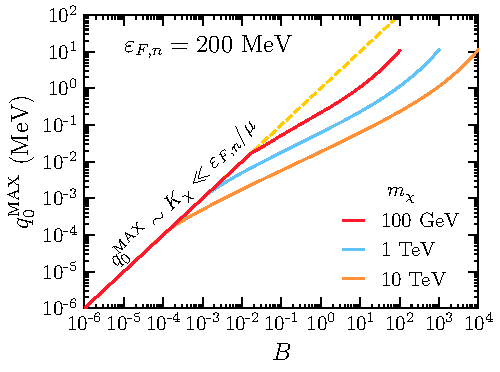
\includegraphics[width=0.49\textwidth]{q0max_Tdm.pdf}
  \caption{Maximum energy loss per collision with neutron targets, as a function of the DM kinetic energy. We have assumed $\kinFn=200\MeV$.} 
  \label{fig:q0max}
\end{figure}
%%%%%%%%%%%%%%%%%%%%%%%%%%%%%%%%%%%%%%%



In either regime, we can obtain first-order approximations for the average fraction of energy that a DM particle loses in a single collision by making use of the zero temperature approximation, a constant target mass, and nucleonic form factors at zero momentum transfer, i.e., $F(t)\sim1$. 
First, we consider the regime in which Pauli blocking is negligible, $m_\chi \gtrsim m_\chi^{\rm crit}$. For a constant cross-section (i.e. $\Msq \propto t^0$) we find 
\begin{equation}
  \langle \Delta K_\chi^{(n=0)} \rangle 
  \sim 2 \sqrt{\frac{\kinFi}{\mu}} K_\chi^{1/2} \ll K_\chi, 
\label{eq:aveElossn0largem}
\end{equation}
at first order in $m_\chi^{\rm crit}/m_\chi$. (See appendix 
% \ref{sec:pauliblockingle} for the corresponding approximation of the interaction rate, Eq.~\ref{eq:intraten0largem}.) 
~\fixMV{ADD APPENDIX} for the corresponding approximation of the interaction rate, Eq.~\fixMV{IN APPENDIX}) 
For cross-sections proportional to $t^1$ and $t^2$, the average energy losses
can be obtained in the same way, starting from the relevant expressions for  $\frac{d\Gamma}{d q_0}$.

Figure~\ref{fig:Taven0} shows the average energy loss fraction per collision. We see the  $\langle \Delta K_\chi^{(n=0)} \rangle/K_\chi \propto K_\chi^{-1/2}$ scaling of Eq.~\ref{eq:aveElossn0largem}
in the $m_\chi \gtrsim m_\chi^{\rm crit}$ phase of the evolution, where the kinetic energy is driven down toward values where Pauli blocking eventually becomes active. The latter Pauli blocked phase is indicated by the horizontal arrows in Fig.~\ref{fig:Taven0}. 





Moving to the case where Pauli blocking suppresses the scattering rate, $m_\chi\lesssim m_\chi^{\rm crit}$, the average energy loss per collision for the case of a constant cross-section is
\begin{equation}
\langle \Delta K_\chi^{(n=0)} \rangle \sim 
\frac{4}{7}K_\chi. 
\label{eq:aveElossn0}
\end{equation}
The average energy loss now scales linearly with $K_\chi$ (the flat regions in Fig.~\ref{fig:Taven0}) in contrast to the $K_\chi^{1/2}$ dependence of Eq.~\ref{eq:aveElossn0largem}.
As the DM kinetic energy decreases, the average fraction of energy transferred to the targets progressively increases until $K_\chi$ no longer satisfies Eq.~\ref{eq:mucrit} and consequently, the interaction rate becomes Pauli blocked.
As expected from Eq.~\ref{eq:mucrit}, the Pauli-suppressed region starts at higher kinetic energy for lower DM masses. 


%%%%%%%%%%%%%%%%%%%%%%%%%%%%%%%%%%%%%%%
\begin{figure}
  \centering
  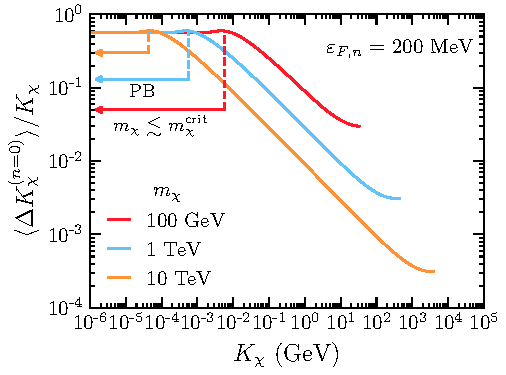
\includegraphics[width=0.49\textwidth]{q0ave_Tdm_n0.pdf}
  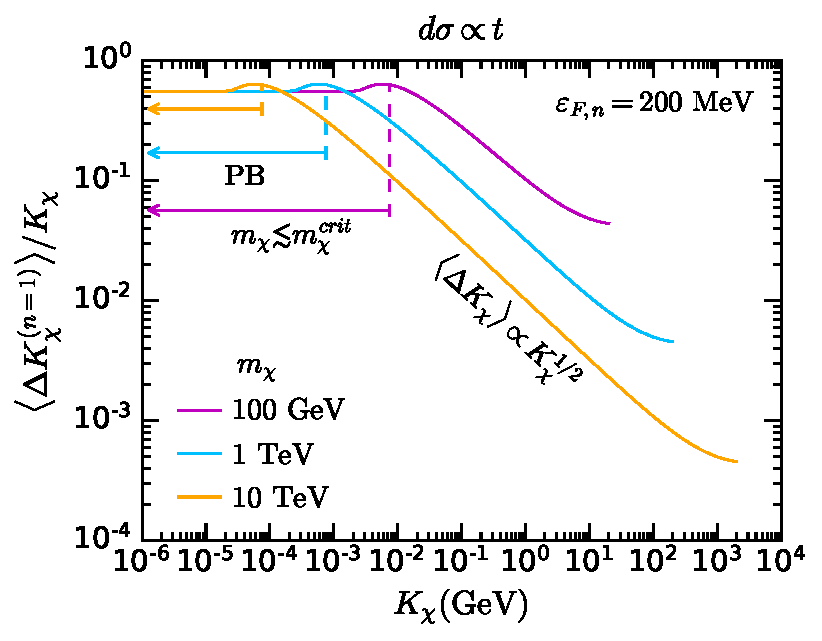
\includegraphics[width=0.49\textwidth]{q0ave_Tdm_n1.pdf}
  \caption{Average fraction of energy loss per DM-neutron collision for constant cross-section (left) and $d\sigma\propto t$ (right) as a function of the DM kinetic energy. Horizontal arrows indicate the Pauli blocked (PB) regime, $m_\chi\lesssim m_\chi^{\rm crit}$. 
  } 
  \label{fig:Taven0}
\end{figure}
%%%%%%%%%%%%%%%%%%%%%%%%%%%%%%%%%%%%%%%




For interactions with $t$-dependent matrix elements, the average energy loss per collision also scales linearly with $K_\chi$ in the Pauli blocked regime. For $\Msq \propto t^n$, with $n=1,2$, we find 
\begin{equation}
  \langle \Delta K_\chi^{(n=1)}\rangle \sim \frac{5}{9}K_\chi, \qquad 
  \langle \Delta K_\chi^{(n=2)} \rangle \sim \frac{28}{55}K_\chi ,
  \label{eq:aveElossn12}
\end{equation}
respectively, where we have used Eqs.~\fixMV{eq:intraten1} and \fixMV{eq:intraten2} for the interaction rates.
Note that the average energy loss fraction per collision exhibits similar behavior for all the interaction types considered,  
as seen by comparing the left and right panels of Fig.~\ref{fig:Taven0}. 
This is true in both the Pauli-blocked and non-blocked regimes.





%%%%%%%%%%%%%%%%%%%%%%%%%%%%%%%%%%%%%%%%%%%%%%%%%%%%%%%%%%%%%%%%%%%%%%%%%%%%%%%%%%%%
%%%%%%%%%%%%%%%%%%%%%%%%%%%%%%%%%%%%%%%%%%%%%%%%%%%%%%%%%%%%%%%%%%%%%%%%%%%%%%%%%%%%
\subsection{Thermalisation timescale}
\label{sec:thermstandard}
%%%%%%%%%%%%%%%%%%%%%%%%%%%%%%%%%%%%%%%%%%%%%%%%%%%%%%%%%%%%%%%%%%%%%%%%%%%%%%%%%%%%
%%%%%%%%%%%%%%%%%%%%%%%%%%%%%%%%%%%%%%%%%%%%%%%%%%%%%%%%%%%%%%%%%%%%%%%%%%%%%%%%%%%%




Once a DM particle is captured, it becomes gravitationally bound to the NS and follows an orbit that may or may not lie completely within the NS. If the orbit lies partly outside the NS, subsequent scatterings will be required for the DM particle to lose enough energy so that the complete orbit lies within the NS. This is the first stage in the thermalisation process. When estimating the amount of time needed for the DM orbit to lie completely within the star,  we find that this time is always much shorter than the full time required for DM to reach thermal equilibrium with the neutron targets. Consequently, this first step in the thermalisation process can be safely neglected. This finding is in agreement with ref.~\cite{Garani:2018kkd_may_NewAnalysisNeutron}. 

We shall also assume that up-scattering of the DM to larger kinetic energy does not play an important role\footnote{Up-scattering refers to collisions with negative energy transfer $q_0<0$, such that the DM particle gains energy instead of losing it. When complete thermalisation has been achieved, the rates for up-scattering and down-scattering must become equal, and hence we expect the up-scattering rates to become more significant as thermalisation is approached.
If this were to be significant, our calculation below would underestimate the full thermalisation time. As we shall see, this does not impact our conclusions.}. These effects will become relevant as the DM approaches thermal equilibrium, increasing the thermalisation time. We estimate that up-scattering will, at most, increase the thermal equilibrium time by $\mathcal{O}(10\%)$, and thus we neglect this correction. 


For DM of mass much larger than the target mass, $m_\chi\gg \mbeff$, there is an additional stage in the thermalisation process where either Pauli blocking plays no role, or the interaction rate has a different power law relationship with the temperature than those identified in Section~\ref{sec:energyloss}. These initial scatterings make a negligible contribution to the thermalisation time, as  $\Gamma^{-}$ is a sharply decreasing function of the DM kinetic energy $K_\chi$. 

 
Let us denote the number of initial collisions before reaching the Pauli blocked regime as $N_1$, and the number of additional collisions required for complete thermalisation as $N_2$. For light DM, $m_\chi\lesssim \mbeff$, Pauli blocking affects the entire thermalisation process, i.e. $N_1=0$. Let $K_N$ be the kinetic energy after $N$ scatterings. After $N_1+N_2$ collisions, the DM will reach the equilibrium temperature $T_{\rm eq}$, which can be written as
\begin{equation}
K_{N_1+N_2} = 
K_{N_1}\left(1-\frac{\langle \Delta K_\chi \rangle}{K_\chi}\right)^{N_2} = \Tstareq,  
\label{eq:Teq}
\end{equation}
where we have used the fact that the average fractional energy loss is the same in each collision. 
The thermalisation time can then be defined as the sum of the average time between collisions, up until the final energy transfer is equal to $T_{\rm eq}$~\cite{Bertoni:2013bsa_dec_DarkMatterThermalization}
\begin{equation}
\tth = \sum_{n=0}^{N_2} \frac{1}{\Gamma^{-}(K_n)} \sim \sum_{n=N_1}^{N_2} \frac{1}{\Gamma^{-}(K_n)}.  
\label{eq:thermtime}
\end{equation}


For  $m_\chi \lesssim m_\chi^{\rm crit}$, the fraction of energy lost in the last few scatters is still a considerable fraction of the DM kinetic energy before the collision. Furthermore, these scatterings may take a considerably long time to occur, indicating that the process is discrete. 
As an example, consider thermalisation to a temperature of $10^3$~K, for a DM particle of mass $m_\chi=1\TeV$ and constant cross-section $\sigma_{n\chi} \sim 10^{-45}\cm^2$.\footnote{ For a wide DM mass range (GeV--TeV), this value is comparable to the cross-section that results in maximal capture, and hence we will use this cross-section as a reference value in some of the estimates that follow.} Hundreds of collisions are required to fully thermalise; the last 10 or so are spaced longer than a second apart; and the last couple are longer than $10 \kyr$ apart.    



To compute the thermalisation time, we numerically integrate Eq.~\ref{eq:diffGammaFiniteTemp} to obtain the interaction rate and the average energy lost in each collision for each of the EFT operators in Table~\ref{tab:opers_defn_full}. We find that the thermalisation time for a particular interaction type scales according to the dominant power of the Mandelstam variable $t$ in the corresponding matrix element; see the last column of  Table~\ref{tab:opers_defn_full}. Thus, to understand how the thermalisation times scale, it is enough to consider differential cross-sections that are proportional to a given power of $t$, i.e. $d\sigma\propto t^n$, with $n=0,1,2$. 
Below, we present results for operators that depend only on $t$ (D1-4 in Table~\ref{tab:opers_defn_full}), and not on the centre of mass energy, $s$. In Appendix~\fixMV{Add s dep appendix}, we outline the procedure used to obtain analytic expressions for those operators with an explicit dependence on $s$ (operators D5-10). 


In Figure~\ref{fig:thermtime}, we show the full numerical results for the thermalisation time as a function of the DM mass for different equilibrium temperatures. It is clear that the power law scaling of the thermalisation time with DM mass depends on whether $m_\chi$ is larger or smaller than the nucleon mass. To understand these results, we make use of the analytic approximations for the average DM energy loss derived in Section~\ref{sec:energyloss} and valid in the zero temperature limit. 

%%%%%%%%%%%%%%%%%%%%%%%%%%%%%%%%%%%%
\begin{figure}
\centering 
  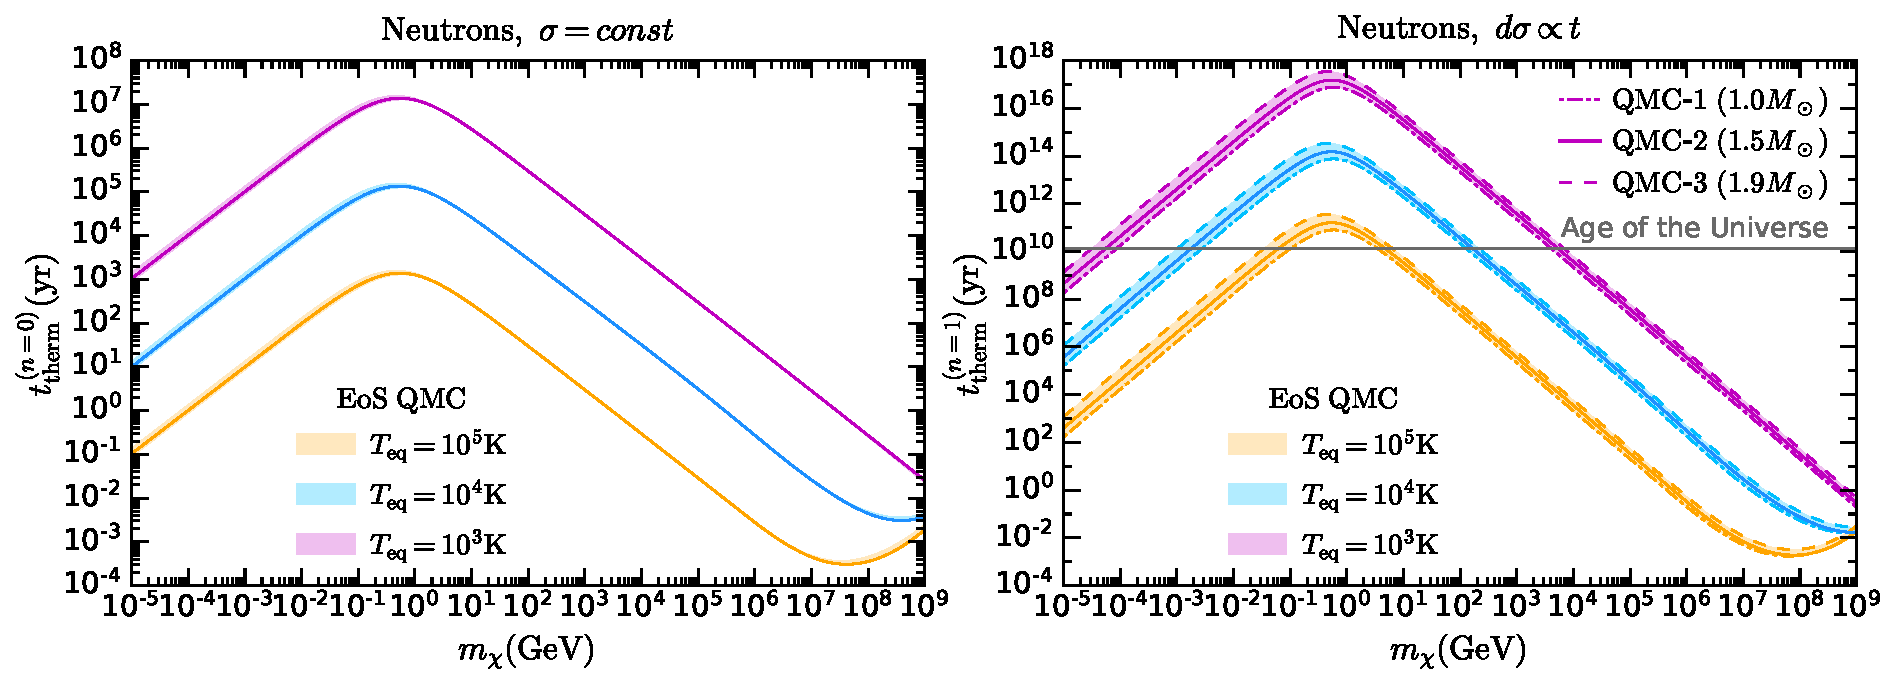
\includegraphics[width=\textwidth]{ttherm_mdm_n0_n1.pdf}
  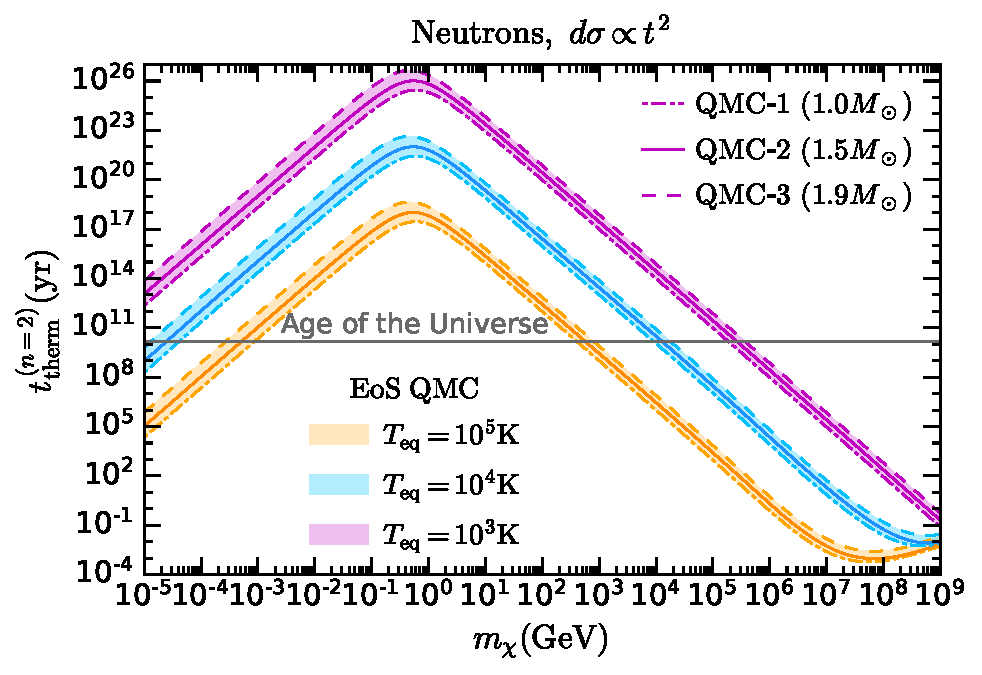
\includegraphics[width=.525\textwidth]{ttherm_n2_eos.pdf}
  \caption{thermalisation time as a function of the DM mass for constant cross-section (top left), $d\sigma \propto t$ (top right)  and $d\sigma\propto t^2$ (bottom). We have used the NS benchmark models in Table~\ref{tab:QMC_configs} and a reference cross-section of $\sigma_{\rm n\chi}= 10^{-45}\cm^2$ close to the NS surface. Shaded regions indicate the variation with the choice of EoS: QMC-1 (dot-dashed), QMC-2 (solid), and QMC-3 (dashed). 
  }
  \label{fig:thermtime}
\end{figure}
%%%%%%%%%%%%%%%%%%%%%%%%%%%%%%%%%%%%


We begin by studying the Pauli blocked regime, $m_\chi \lesssim m_\chi^{\rm crit}$. 
In this case, the majority of the thermalisation time is dictated by the final few scatters, for which the form factors are close to their value at zero momentum transfer.  These last collisions occur close to the NS centre, so we can take the target mass as constant and equal to the value at the centre of the star, $\mbeff(0)$. For the case of a constant DM-neutron cross-section, $d\sigma \propto t^0$, the thermalisation time can thus be obtained by using  Eqs.~\fixMV{eq:intraten0}, \ref{eq:Teq} and \ref{eq:aveElossn0} in Eq.~\ref{eq:thermtime}. This leads to
%
\footnotesize
\begin{equation}
  \tthn{0} \sim   \frac{147}{16 }\frac{\pi^2 m_\chi}{ \left(\mbeff(0) + m_\chi\right)^2}\frac{1}{\sigma_{i\chi}^{n=0}}\frac{1}{T_{\rm eq}^2}, 
  \label{eq:thermtimen0}
\end{equation} 
\normalsize
%
where $\sigma_{i\chi}^{n=0}$ is the DM-baryon cross-section. 
The scaling of this expression with $\Tstareq$, DM mass, and DM-target cross-sections 
agrees with ref.~\cite{Bertoni:2013bsa_dec_DarkMatterThermalization}. 
Numerically we obtain
\footnotesize
\begin{equation}
  \tthn{0} \sim \begin{dcases}
    4.4\times 10^{6}\yrs \, \left(\frac{m_\chi}{10\MeV}\right)\left(\frac{10^{-45}\cm^2}{\sigma_{i\chi}^{n=0}}\right)\left(\frac{10^3K}{T_{\rm eq}}\right)^{2},\quad m_\chi \ll \mbeff(0)\\
    9.7\times 10^{6}\yrs \, \left(\frac{10\GeV}{m_\chi}\right)\left(\frac{10^{-45}\cm^2}{\sigma_{i\chi}^{n=0}}\right)\left(\frac{10^3K}{T_{\rm eq}}\right)^{2},\quad m_\chi \gg \mbeff(0)
  \end{dcases} \label{eq:t_therm_0}
\end{equation}
\normalsize
%
where we have set $\mbeff(0) = 0.5\,m_n$. 
The $m_\chi$ dependence of these expressions explains the features observed in the top left panel of Fig.~\ref{fig:thermtime}. For $m_\chi \ll \mneff(0)$, the thermalisation time scales with the DM mass as the number of scatterings needed for thermalisation increases. Conversely, for $m_\chi \gg \mneff(0)$, $\tthn{0}$ is inversely proportional to $m_\chi$ due to the reduced Pauli blocking, explaining the change of slope around the value of the neutron effective mass in the NS centre. 




We repeat the same analysis for cross-section proportional to higher powers of $t$, i.e., $d\sigma \propto t^n$ with $n=1,2$. Using Eqs.~\fixMV{eq:intraten1}, \fixMV{eq:intraten2} and \ref{eq:aveElossn12}, we find
% 
\small
\begin{align}
    \tthn{1} &\sim 14 %\frac{2187}{152}
    \frac{\pi^2 m_\chi^2 (\mbeff(0))^2}{\left(\mbeff(0) + m_\chi\right)^2 \left((\mbeff(0))^2+ m_\chi^2\right)}\frac{1}{\sigma_{i\chi}^{n=1}}\frac{1}{T_{\rm eq}^3} \frac{1-B(\Rstar)}{B(\Rstar)},  
    \label{eq:thermtimen1}\\
    \tthn{2} &\sim 17 %\frac{27451875}{1231312}
    \frac{\pi^2 m_\chi^3 (\mbeff(0))^4}{\left(\mbeff(0) + m_\chi\right)^2 \left((\mbeff(0))^2+ m_\chi^2\right)^2}\frac{1}{\sigma_{i\chi}^{n=2}}\frac{1}{T_{\rm eq}^4} \left[\frac{1-B(\Rstar)}{B(\Rstar)}\right]^2, 
    \label{eq:thermtimen2}
\end{align}
\normalsize
% 
where the factors involving $B(R_\star)$ arise from fixing the cross-section to its value at the surface; 
see Appendix~\fixMV{sec:pauliblockingle} for details.


To gain insight into the order of magnitude of these thermalisation times, we set  $B(\Rstar)=0.5$ and $\mbeff(0) = 0.5\,m_n$, yielding
% 
\footnotesize{
\begin{align}
    \tthn{1} &\sim \begin{dcases}
        2.5\times 10^{14}\yrs \, \left(\frac{m_\chi}{10\MeV}\right)^2\left(\frac{10^{-45}\cm^2}{\sigma_{i\chi}^{n=1}}\right)\left(\frac{10^3K}{T_{\rm eq}}\right)^{3},\quad m_\chi \ll \mbeff(0)\\
        3.9\times 10^{15}\yrs \, \left(\frac{10\GeV}{m_\chi}\right)^2\left(\frac{10^{-45}\cm^2}{\sigma_{i\chi}^{n=1}}\right)\left(\frac{10^3K}{T_{\rm eq}}\right)^{3},\quad m_\chi \gg \mbeff(0)
    \end{dcases}
    \label{eq:t_therm_1} \\
   \tthn{2} &\sim\begin{dcases}
        1.1\times 10^{23}\yrs \, \left(\frac{m_\chi}{10\MeV}\right)^3\left(\frac{10^{-45}\cm^2}{\sigma_{i\chi}^{n=2}}\right)\left(\frac{10^3K}{T_{\rm eq}}\right)^{4},\quad m_\chi \ll \mbeff(0)\\
        1.2\times 10^{24}\yrs \, \left(\frac{10\GeV}{m_\chi}\right)^3\left(\frac{10^{-45}\cm^2}{\sigma_{i\chi}^{n=2}}\right)\left(\frac{10^3K}{T_{\rm eq}}\right)^{4},\quad m_\chi \gg \mbeff(0).
    \end{dcases}
    \label{eq:t_therm_2}
\end{align} 
}
\normalsize
% 
As anticipated, we see that the momentum-suppressed cross-sections translate into significantly longer thermalisation times than for the case of a constant (unsuppressed) cross-section.
These expressions also allow us to understand the dependence of $\tth$ on the DM mass.
For $d\sigma\propto t^n$, the thermalisation time scales as $m_\chi^{n+1}$ for $m_\chi \ll \mneff(0)$, and as the inverse of this quantity for $m_\chi \gg \mneff(0)$.



The choice of EoS has a small but non-negligible impact on the thermalisation time, as indicated by the widths of the shaded regions in Fig.~\ref{fig:thermtime}. 
For a constant cross-section, we observe almost no variation in $\tth$ with the NS configuration, except for the $m_\chi \lesssim m_n$ region. This is due to the dependence of $\mneff(0)$ on the NS model; see Table~\ref{tab:QMC_configs} and Eq.~\ref{eq:thermtimen0}.
For cross-sections $d\sigma\propto t^n$, with $n=1,2$, the dependence on $B(\Rstar)$ in Eqs.~\ref{eq:thermtimen1} and \ref{eq:thermtimen2} adds an extra dependence on the choice of NS model. For these momentum-suppressed interactions, DM requires more time to reach an equilibrium temperature in heavier NSs. This is due to the combination of two effects: the effective mass of the targets in the centre of the NS is smaller in more massive NS configurations, while $B(\Rstar)$ increases. Nonetheless, the dependence on NS configuration remains relatively mild. 

%%%%%%%%%%%%%%%%%%%%%%%%%%%%%%%%%%%%%



We now turn to the $m_\chi \gtrsim \mcrit$ regime, which is observed only for temperatures above $10^4\K$ in Fig.~\ref{fig:thermtime}. This regime change is indicated by the change of slope that occurs at large DM masses, clearly evident for  $T_{eq}=10^5\K$ (orange)  at a DM of mass $m_\chi\gtrsim5\times10^7\GeV$.  
In this regime, the energy lost in each collision is a tiny fraction of the initial DM kinetic energy, and the time between scatterings is of order a fraction of a second. This indicates that a continuous approximation becomes more appropriate than a discrete sum to estimate $\tth$.
In this case, the momentum-dependent part of the form factor, $F(t)$, will be relevant only at the beginning of the thermalisation process and become less and less relevant as the average momentum transfer decreases in each subsequent scatter.\footnote{We have numerically verified that the $t$-dependent form factors do not alter the results in any significant manner.} It is these low momentum-transfer collisions that dominate the thermalisation time.
%
For a constant cross-section ($n=0$), in the zero temperature approximation, we obtain 
(see Appendix~\fixMV{sec:thermsuperheavy} for details)
\begin{equation}
    \tthn{0} \sim \frac{9 \pi^2 m_\chi}{8 (\mbeff(0))^2 \kinFi^2 \sigma_{i\chi}^{n=0} }\log\left[\frac{m_\chi}{T_{\rm eq}}\left(\frac{1}{\sqrt{B(\Rstar)}}-1\right)\right]. %\quad m_\chi\gtrsim m_\chi^{\rm crit}.
\label{eq:tthemheavy0text}
\end{equation}
In this super heavy DM mass regime, we see that the thermalisation time is an increasing function of $m_\chi$. 


It is worth remarking that for a constant DM-neutron cross-section (top left panel) thermalisation will always occur within the age of the Universe. However, this is not true for momentum-suppressed cross-sections, for a range of DM masses. Specifically, for $T_{\rm eq}=10^3\K$ and the assumed reference cross-section,  DM of mass $m_\chi\lesssim 10 \TeV$ ($m_\chi\lesssim 1 \PeV$)  will not have enough time to  thermalise  for $d\sigma \propto t$ ($d\sigma \propto t^2$).
Importantly, however, we shall see below that even when full thermalisation takes longer than the age of the Universe, the majority of the kinetic energy is deposited on a much shorter timescale.



Finally, we must incorporate the fact that DM will scatter with various baryonic species in the NS rather than just the neutrons. To do this, the thermalisation times from scattering off each species are combined appropriately based on their abundances. Specifically, we sum the inverse single-species thermalisation times, weighted by their relative abundance at the centre of the NS, such that
\begin{equation}
    \frac{1}{t_{\text{therm},\; \text{tot}}} = \sum_i \frac{Y_i(0)}{t_{\text{therm},\;i}},
    \label{eq:tthermtot}
\end{equation}
where $Y_i(0)$ is the abundance of the species in the centre of the NS, and the sum runs over all possible baryons. For the case of the heaviest NS we consider, 1.9 $\Msun$, this includes the $\Lambda^0$, $\Xi^0$ and $\Xi^-$ hyperons. The resulting thermalisation time then lies between the fastest and slowest single-species times, as is expected.










%%%%%%%%%%%%%%%%%%%%%%%%%%%%%%%%%%%%%%%%%%%%%%%%%%%%%%%%%%%%%%%%%%%%%%%%%%%%%%%%%%%%
%%%%%%%%%%%%%%%%%%%%%%%%%%%%%%%%%%%%%%%%%%%%%%%%%%%%%%%%%%%%%%%%%%%%%%%%%%%%%%%%%%%%
\section{Capture-Annihilation Equilibrium}
\label{sec:CAEquilibrium}
%%%%%%%%%%%%%%%%%%%%%%%%%%%%%%%%%%%%%%%%%%%%%%%%%%%%%%%%%%%%%%%%%%%%%%%%%%%%%%%%%%%%
%%%%%%%%%%%%%%%%%%%%%%%%%%%%%%%%%%%%%%%%%%%%%%%%%%%%%%%%%%%%%%%%%%%%%%%%%%%%%%%%%%%%




The captured DM will accumulate in the centre of the NS, where it will begin to annihilate. The annihilation rate will grow until sufficient time has elapsed for the capture and annihilation processes to reach equilibrium. In this limit, the total amount of DM in the NS is maximised and will remain constant. Once this occurs, annihilation efficiently deposits the DM mass-energy into the star. 


Let us begin by assuming that the dark matter has fully thermalised. After reviewing the standard capture-annihilation equilibrium calculation, we will relax this assumption to consider the more general case of partially thermalised dark matter and derive new expressions that hold in that scenario. Importantly, we shall see that capture-annihilation equilibrium, and hence efficient annihilation can occur without full thermalisation.

%%%%%%%%%%%%%%%%%%%%%%%%%%%%%%%%%%%%%%
\subsection{Capture-annihilation equilibrium of thermalised dark matter}
%%%%%%%%%%%%%%%%%%%%%%%%%%%%%%%%%%%%%%


The thermalised DM will collect within an isothermal sphere at the centre of the NS where it will begin to annihilate. The efficiency of the annihilation will depend on the volume of this sphere, which is expected to be very small for the DM masses we consider. 
Very close to the centre of the NS, the density does not vary significantly and can be taken to be constant. Then, working in the weak field approximation such that $B(r) \sim  1+2\Phi(r)$, 
we can obtain the gravitational potential inside the NS,
\begin{align}
\Phi(r) & = -\int_r^\infty \frac{G M_\star(r')}{r'^2}dr' 
\approx \frac{2}{3}\pi G \rho_c r^2, 
\end{align}
where $\rho_c$ is the central density of the NS. 
The  number density of DM particles that have thermalised to a temperature $\Tstareq$ as a function of radius will then be given by a Maxwell-Boltzmann distribution
\begin{align}
n_{\chi}(r) & \simeq n_0 \exp\left[ -\frac{m_\chi\Phi(r)}{T_{\rm eq}}\right] 
= \frac{N_\chi}{\pi^{3/2}  r_{\rm iso}^3}\exp\left( -\frac{r^2}{ r_{\rm iso}^2}\right), 
\end{align}
where $N_\chi$ is the total number of DM particles within the isothermal sphere, and $r_{\rm iso}$ is the radius of the DM isothermal sphere. 
Applying the viral theorem leads to the following expression for $r_{\rm iso}$, 
\begin{align}
r_{\rm iso} & = \sqrt{\frac{3 \Tstareq}{2\pi G m_\chi \rho_c}} \nonumber\\
& \approx  0.26\,\text{m}\left[\left(\frac{T_{\rm eq}}{10^3\,\text{K}}\right)\left(\frac{1\GeV}{m_\chi}\right)\left(\frac{8\times10^{14}\,\textrm{g}\,\text{cm}^{-3}}{\rho_c}\right)\right]^{1/2}.
\end{align}
The total number of DM particles enclosed in this sphere is then
\begin{equation}
    N_\chi    \simeq  4\pi\int dr \, r^2n_{\chi}(r),
\end{equation} 
and the velocity distribution of the thermalised DM is  given by
\begin{equation}
f_{\rm MB}(v_\chi)  = 4\pi \left(\frac{m_\chi}{4 \pi \Tstareq}\right)^{3/2} v_\chi^2 \exp\left[ -\frac{m_\chi v_\chi^2}{4 \Tstareq} \right].
\end{equation}




In the absence of evaporation, which can safely be neglected for $m_\chi \gtrsim 1.17\times 10^{-8}\GeV$ for a Gyr old NS with core temperature $\sim 10^3\K$~\cite{Bell:2020lmm_mar_ImprovedTreatmentDark}, the time evolution of the total number of DM particles present inside the NS is governed by
\begin{equation}
    \frac{dN_\chi}{dt} = C - A N_\chi^2 \label{eq:ndm}.
\end{equation}
Here $C$ is the capture rate and  $A$ is related to the DM annihilation rate, $\Gamma_{\rm ann}$, through
\begin{equation}
    \Gamma_{\rm ann} =  \frac{1}{2}A N_\chi^2,
\end{equation}
where
\begin{equation}
    A = \frac{\langle \sigma_\text{ann}v_\chi \rangle}{N_\chi^2} \int n_\chi^2(r) d^3 r \simeq \frac{\langle \sigma_\text{ann} v_\chi\rangle}{(2\pi)^{3/2} r_{\rm iso}^3}, \label{eq:annrate}
\end{equation}
and $\langle \sigma_{\rm ann} v_\chi \rangle$ is the
thermally averaged DM annihilation cross-section. These are given in Table~\ref{tab:annCS} for the EFT interactions we consider, where $\langle v^2_\chi \rangle = v_{\rm th}^2 =  6 \Tstareq/ m_\chi$.


We note that the cross-sections shown in Table~\ref{tab:annCS} are quark-level expressions. For most of the mass range of interest, these provide excellent approximations to the hadron-level annihilation cross-sections, provided we impose a lower bound on the DM mass for which an annihilation channel is open, taken to be the pion mass. See Appendix~\fixMV{sec:quarkhadron} for details.




%%%%%%%%%%%%%%%%%%%%%%%%%%%%%%%%%%%%%%%%%%%%%%%%%%%%%%%%%%%%%%%%
\begin{table}[t]
    \centering
    \begin{tabular}{c c l}
    \toprule
         Name & Operator & $\langle \sigma_{ann} v_\chi\rangle$\\
        \midrule\midrule 
         D1  & $\bar\chi  \chi\;\bar q  q $ & 
         $\frac{3 m_\chi^2}{8\pi\Lambda^4}\sum_q y_q^2 \left( 1 - \frac{m_q^2}{m_\chi^2}\right)^{3/2} v_{\rm th}^2 $\\ 
         D2  &  $\bar\chi \gamma^5 \chi\;\bar q q $ & \small $\frac{3 m_\chi^2}{2\pi \Lambda^4}\sum_q y_q^2 \sqrt{1 - \frac{m_q^2}{m_\chi^2}} \left[ \left( 1 - \frac{m_q^2}{m_\chi^2}\right) + \frac{3}{8}\frac{m_q^2}{m_\chi^2}v_{\rm th}^2\right]$\\
         D3  & $\bar\chi \chi\;\bar q \gamma^5  q $  & \small $\frac{3 m_\chi^2}{8\pi\Lambda^4}\sum_q y_q^2 \sqrt{ 1 - \frac{m_q^2}{m_\chi^2}} v_{\rm th}^2$\\
         D4  & $\bar\chi \gamma^5 \chi\; \bar q \gamma^5 q $ & \small $ \frac{3 m_\chi^2}{2\pi\Lambda^4}\sum_q y_q^2 \sqrt{1 - \frac{m_q^2}{m_\chi^2}}\left[ 1 + \frac{m_q^2}{8(m_\chi^2 - m_q^2)} v_{\rm th}^2\right]$\\
         D5  & $\bar \chi \gamma_\mu \chi\; \bar q \gamma^\mu q$ & \small $\frac{3 m_\chi^2}{2\pi \Lambda^4}\sum_q \sqrt{1 - \frac{m_q^2}{m_\chi^2}} \left[ \left( 2 +\frac{m_q^2}{m_\chi^2}\right) + \left( \frac{-4m_\chi^4 +2m_q^2 m_\chi^2 +11m_q^4}{24m_\chi^2 ( m_\chi^2 - m_q^2)} \right) v_{\rm th}^2 \right]$\\
         D6  & $\bar\chi \gamma_\mu \gamma^5 \chi\; \bar  q \gamma^\mu q $ & \small $\frac{m_\chi^2}{4\pi \Lambda^4}\sum_q \sqrt{1 - \frac{m_q^2}{m_\chi^2}} \left[ 2 +\frac{m_q^2}{m_\chi^2}\right] v_{\rm th}^2$\\
         D7  & $\bar \chi \gamma_\mu  \chi\; \bar q \gamma^\mu\gamma^5  q$  & \small $ \frac{3 m_\chi^2 }{\pi\Lambda^4}\sum_q \sqrt{1 - \frac{m_q^2}{m_\chi^2}} \left[ \left( 1 - \frac{m_q^2}{m_\chi^2} \right) - \frac{1}{24}\left( 2 - 11\frac{m_q^2}{m_\chi^2}\right) v_{\rm th}^2 \right]$ \\
         D8  & $\bar \chi \gamma_\mu \gamma^5 \chi\; \bar q \gamma^\mu \gamma^5 q $ & \small $ \frac{3 m_\chi^2}{2\pi \Lambda^4} \sum_q \sqrt{1 - \frac{m_q^2}{m_\chi^2}} \left[ \frac{m_q^2}{m_\chi^2} + \left( \frac{8m_\chi^4 - 28m_\chi^2 m_q^2 + 23 m_q^4}{24 m_\chi^2(m_\chi^2 - m_q^2)} \right) v_{\rm th}^2 \right] $ \\
         D9  & $\bar \chi \sigma_{\mu\nu} \chi\; \bar q \sigma^{\mu\nu} q $  & \small $ \frac{6 m_\chi^2}{\pi\Lambda^4} \sum_q \sqrt{1 - \frac{m_q^2}{m_\chi^2}} \left[ \left( 1 + 
         2\frac{m_q^2}{m_\chi^2}\right) -\left( \frac{2m_\chi^4 +17m_q^2 m_\chi^2 -28m_q^4}{24m_\chi^2(m_\chi^2 - m_q^2) }\right) v_{\rm th}^2\right] $ \\     
         D10 & $\bar \chi \sigma_{\mu\nu} \gamma^5\chi\; \bar q \sigma^{\mu\nu} q$ & \small $\frac{6 m_\chi^2}{\pi\Lambda^4} \sum_q \sqrt{1 - \frac{m_q^2}{m_\chi^2}} \left[ \left( 1 - \frac{m_q^2}{m_\chi^2}\right)  -\frac{1}{24}\left(2 -17\frac{m_q^2}{m_\chi^2}\right) v_{\rm th}^2 \right] $\\
         \bottomrule
    \end{tabular}
    \caption{Thermally averaged annihilation cross-sections $\sigmav$ for the dimension 6 EFT operators, expanded to second order in $v_\chi$. The $y_q$ factors are the quark Yukawa couplings~\cite{Zheng:2010js_Constraininginteractionstrength}.}
    \label{tab:annCS} 
\end{table}
%%%%%%%%%%%%%%%%%%%%%%%%%%%%%%%%%%%%%%%%%%%%%%%%%%%%%%%%%%%%%%%%




The solution to Eq.~\ref{eq:ndm} in terms of the capture and annihilation rates is
%
\begin{equation}
    N_\chi(t) = \sqrt{\frac{C}{A}}\tanh\left(\sqrt{CA} \,t\right).\label{eq:Noft}
\end{equation}
%
Ultimately, we are interested in the behavior of Eq.~\ref{eq:Noft} at late stages in the NS evolution, i.e., for $t\rightarrow \tstar$, where $\tstar$ is the age of the NS, which we take to be $\sim 1\Gyr$. In this limit, the hydrostatic NS structure, and hence the capture rate, are not expected to change with time. Of particular interest is whether or not an equilibrium is reached between the capture and annihilation rates. Such a state is reached for timescales greater than 
\begin{equation}
     t_{\rm eq} = \frac{1}{\sqrt{C A}}.
     \label{eq:teqold}
\end{equation}
For earlier times, $ t < t_{\rm eq}$, one can neglect the loss of DM particles due to annihilation, leaving $N_\chi\sim C t$. 


%%%%%%%%%%%%%%%%%%%%%%%%%%%%%%%%%%%%%%
\subsection{Capture-annihilation equilibrium of partially\\ thermalised dark matter}
%%%%%%%%%%%%%%%%%%%%%%%%%%%%%%%%%%%%%%



The standard calculation of the annihilation rate, using Eq.~\ref{eq:annrate}, assumes that the DM has thermalised, i.e., $t > t_{\rm therm}$. 
If thermalisation has not been achieved by a time $t\sim\tstar<\tth$, the DM kinetic energy distribution will peak around the lowest temperature that DM has had enough time to reach. This is given by 
%
\begin{equation}
K_\chi \sim T_{\rm eq} \left(\frac{\tth+\tstar}{\tstar}\right)^{\frac{1}{2+n}},
\label{eq:lowtemp}
\end{equation}
%
where $n$ is the exponent of the dominant $t^n$ term in the differential cross-section, $d\sigma \propto t^n$, as given in the last column of Table~\ref{tab:opers_defn_full}. See Appendix~\fixMV{sec:minTempDerivation} for details. 
We can then find the radius of the DM distribution (which is no longer isothermal) and the $\sigmav$ corresponding to the peak of the energy distribution $K_\chi$. 
We obtain $A$ via the replacement  
%
\begin{equation}
    A \rightarrow A \left(\frac{T_\text{eq}}{K_\chi}\right)^{\alpha} = 
   A \left(\frac{\tstar}{t_\text{therm}+\tstar}\right)^{\frac{\alpha}{2+n}},  
\end{equation}
%
where $\alpha=3/2$ for $s$-wave annihilation, and $\alpha=1/2$ for $p$-wave. 
Making this replacement in Eq.~\ref{eq:teqold} leads to a capture-annihilation equilibrium time of
\begin{equation}
 t_{\rm eq} = \frac{1}{\sqrt{C A}} \left(\frac{t_\text{therm}+\tstar}{\tstar}\right)^{\frac{\alpha}{2(2+n)}}. \label{eq:teq} 
\end{equation}

No previous estimate of the capture-annihilation equilibrium time has considered the case of partially thermalised DM. If thermalisation has not been achieved, the additional factor in Eq.~\ref{eq:teq}, compared to Eq.~\ref{eq:teqold}, increases the equilibrium time. (Or, equivalently, increases the cross-sections required to reach equilibrium within a specified time.) However, it is critical to realize that $t_\text{eq}$ can be shorter than $t_\text{therm}$. 
In fact, annihilation can occur efficiently even if complete thermalisation never occurs. In this scenario, we must use Eq.~\ref{eq:teq}.



Assuming the DM is captured at the geometric limit, we arrive at the following result for our benchmark NS QMC-2
\begin{eqnarray}
    t_{\rm eq}  &\sim&  4\times10^{-6}\yr\left(\frac{100\GeV}{m_\chi}\right)^{\frac{1}{4}}\left(\frac{10^{-26}\cm^3 \s^{-1}}{\langle\sigma_\text{ann} v_\chi\rangle}\right)^{\frac{1}{2}} \left(\frac{1\GeV\cm^{-3}}{\rho_\chi}\right)^{\frac{1}{2}}\left(\frac{T_{\rm eq}}{10^3\K}\right)^{\frac{3}{4}} 
    \nonumber \\ &&\times
    \left(\frac{t_{\rm therm}+\tstar}{\tstar}\right)^{\frac{\alpha}{2(2+n)}}.
\end{eqnarray}
Comparing this expression with the thermalisation times in the previous section, we anticipate that  $t_\text{eq}$ will typically be shorter than $t_\text{therm}$, often by many orders of magnitude.




%%%%%%%%%%%%%%%%%%%%%%%%%%%%%%%%%%%%%%%%%%%%%%%%
%%%%%%%%%%%%%%%%%%%%%%%%%%%%%%%%%%%%%%%%%%%%%%%%
\section{Neutron Star Heating Timescales}
\label{sec:results}
%%%%%%%%%%%%%%%%%%%%%%%%%%%%%%%%%%%%%%%%%%%%%%%%
%%%%%%%%%%%%%%%%%%%%%%%%%%%%%%%%%%%%%%%%%%%%%%%%



%%%%%%%%%%%%%%%%%%%%%%%%%%%%%%%%%%%%%%%%%%%%%%%%
\subsection{Kinetic heating timescale}
\label{subsec:KinHeating}
%%%%%%%%%%%%%%%%%%%%%%%%%%%%%%%%%%%%%%%%%%%%%%%%


It has commonly been assumed that the DM kinetic energy deposition occurs instantaneously. However, it is not immediately obvious that this is true. In particular, for scattering interactions suppressed by powers of the momentum transfer, $t$, full thermalisation can take longer than the age of the Universe. We must therefore determine whether a {\it significant fraction} of the initial kinetic energy can be deposited on a shorter timescale.



To quantify the timescale on which kinetic heating takes place, we define $t_{\rm kin}$ to be the time required for a DM particle to lose 99\% of its maximum kinetic energy, $K_\chi = m_\chi (1/\sqrt{B(0)} - 1)$.  
This time is calculated in the same way as the thermalisation time, while also keeping track of the time the DM spends outside the star along its orbit, i.e., the initial stage of the thermalisation process that was neglected in Section~\ref{sec:thermstandard}. For simplicity, the DM particle orbits are taken to be linear, passing through the centre of the star, with the radial extent calculated using the geodesic equations. We expect an ${\cal O}(1)$ correction to our results when considering circular orbits.
Additionally, we randomize the radial position in the NS where the DM interacts with a target. 

%%%%%%%%%%%%%%%%%%%%%%%
\begin{figure}[t] 
    \centering  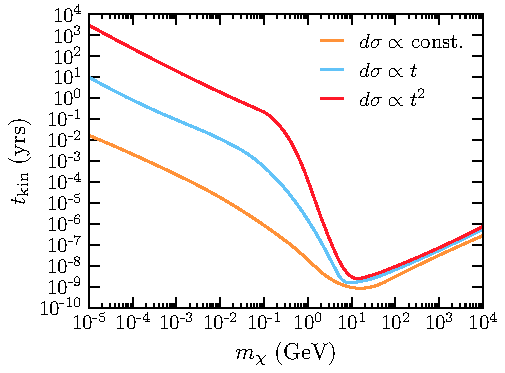
\includegraphics[width=.5\textwidth]{kinheattime_mdm.pdf}
    \caption{Timescale on which the DM deposits $99\%$ of its initial kinetic energy in the NS. We have assumed an NS with configuration QMC-2, and a DM-neutron scattering cross-section of $\sigma_{n\chi}=10^{-45}\cm^2$ at the surface of the star. 
    }
    \label{fig:kinheattimes}
\end{figure}
%%%%%%%%%%%%%%%%%%%%%%%

Figure~\ref{fig:kinheattimes} shows the time required for kinetic heating to be achieved, assuming DM-neutron interactions of the form $d\sigma \propto t^n$, with cross-sections normalized to $\sigma_{n\chi} = 10^{-45}\cm^2$ at the surface of the star. As the location of each interaction is randomized, these results are obtained by averaging over several simulations for each DM mass. For light DM, $t_{\rm kin}$ decreases with increasing DM mass, due to the decreased effects of Pauli blocking, with the change of slope at $m_\chi \sim 0.1\GeV$ indicating the point where Pauli blocking affects only a fraction of the total process.
For masses $\gtrsim 10\GeV$, Pauli blocking is not relevant to this part of the thermalisation process, and hence the $t_{\rm kin}$ monotonically increases with the DM mass, as was seen in the thermalisation of super-heavy DM. 

Fig.~\ref{fig:kinheattimes} illustrates two key facts. First, $t_{\rm kin}$ differs by orders of magnitude for the different cross-section types, $d\sigma\propto t^n$, with larger values of $t_{\rm kin}$ for the most highly momentum-suppressed interactions, as expected. Second, and importantly, the kinetic heating occurs relatively quickly for all interaction types, on timescales much shorter than a typical NS age. Indeed, for the case of a constant cross-section, $\tkin$ is much shorter than a year.



%%%%%%%%%%%%%%%%%%%%%%%%%%%%%%%%%%%%%%%%%%%%%%%%
\subsection{Annihilation heating timescale}
\label{subsec:AnnHeatTimes}
%%%%%%%%%%%%%%%%%%%%%%%%%%%%%%%%%%%%%%%%%%%%%%%%



%%%%%%%%%%%%%%%%%%%%%%%%%%
\begin{figure}[t]
\centering    
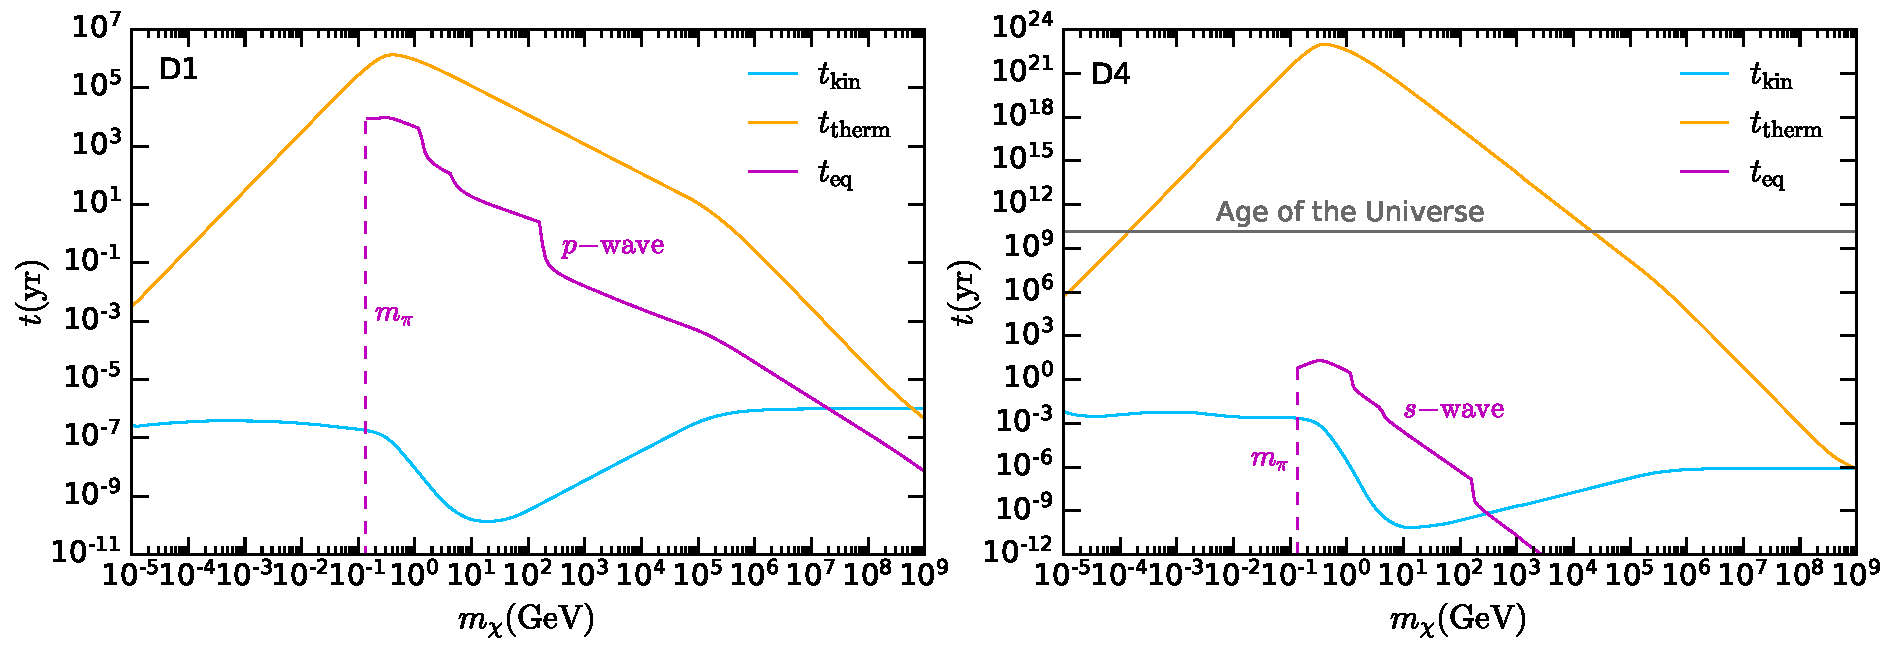
\includegraphics[width=\textwidth]{timescales_maxcap_n.pdf}
    \caption{Timescales for kinetic heating (blue), thermalisation (orange), and capture-annihilation equilibrium (magenta), for operators D1 (left) and D4 (right). The operator D1 has an unsuppressed scattering cross-section and a $p$-wave suppressed annihilation cross-section, while $D4$ has a $q_\text{tr}^4$ suppressed scattering cross-section and an unsuppressed ($s$-wave) annihilation cross-section.
    The interaction strength has been chosen to give maximal capture. (Specifically, we used $\Lambda_q$ values corresponding to a capture cross-section at the geometric limit, assuming scattering with the neutron targets in the QMC-2 NS.)   
    }
    \label{fig:timescales}
\end{figure}
%%%%%%%%%%%%%%%%%%%%%%%%%%



Figure~\ref{fig:timescales} shows all relevant timescales for DM-induced heating of old neutron stars. These timescales have been calculated considering DM scattering off the neutron targets in the benchmark NS QMC-2, for the case of maximal capture, $f = 1$ (i.e., we have set the EFT parameter $\Lambda_q$ as required to achieve capture at the geometric limit).
We show these results for two indicative operators: The scalar-scalar interaction D1 (left), which has a $p$-wave suppressed annihilation cross-section, and the pseudoscalar-pseudoscalar operator D4 (right), which has an $s$-wave annihilation cross-section. 

As anticipated, capture-annihilation equilibrium takes longer to achieve for the velocity-suppressed $p$-wave annihilation cross-section than for the $s$-wave.  Nonetheless,  
equilibrium (and hence maximal annihilation heating) is reached relatively quickly in both cases, on timescales of $10^4$ years for the scalar interaction, and even quicker for the pseudoscalar, well within the age of a typical NS. 


For both interaction types, the kinetic and annihilation heating contributions are both realized on timescales much shorter than that required for full thermalisation. If the scattering cross-section is momentum suppressed (as with the $d\sigma \propto t^2=q_\text{tr}^4$ dependence for D4), the thermalisation time is increased; if the annihilation cross-section is velocity suppressed (as with the $p$-wave annihilation cross-section for D1) the capture-annihilation equilibrium time is increased.


 
Finally, note that there are parameters for which the annihilation timescale $\teq$ is shorter than the kinetic heating timescale $\tkin$. In this case, the annihilation process deposits the DM mass energy and any remaining kinetic energy, which is carried by the annihilation products. Therefore, the minimum time required for DM to deposit {\it all} of its energy, both kinetic and rest-mass, is $\teq$.


%%%%%%%%%%%%%%%%%%%%%%%%%%%%%%%%%%%
\subsection{Neutron star heating sensitivity for various interaction types}   
\label{ref:heatingresults}
%%%%%%%%%%%%%%%%%%%%%%%%%%%%%%%%%%%


%%%%%%%%%%%%%%%%%%%%%%%%%%%%%%%%%%%
\begin{figure}[t]
    \centering
    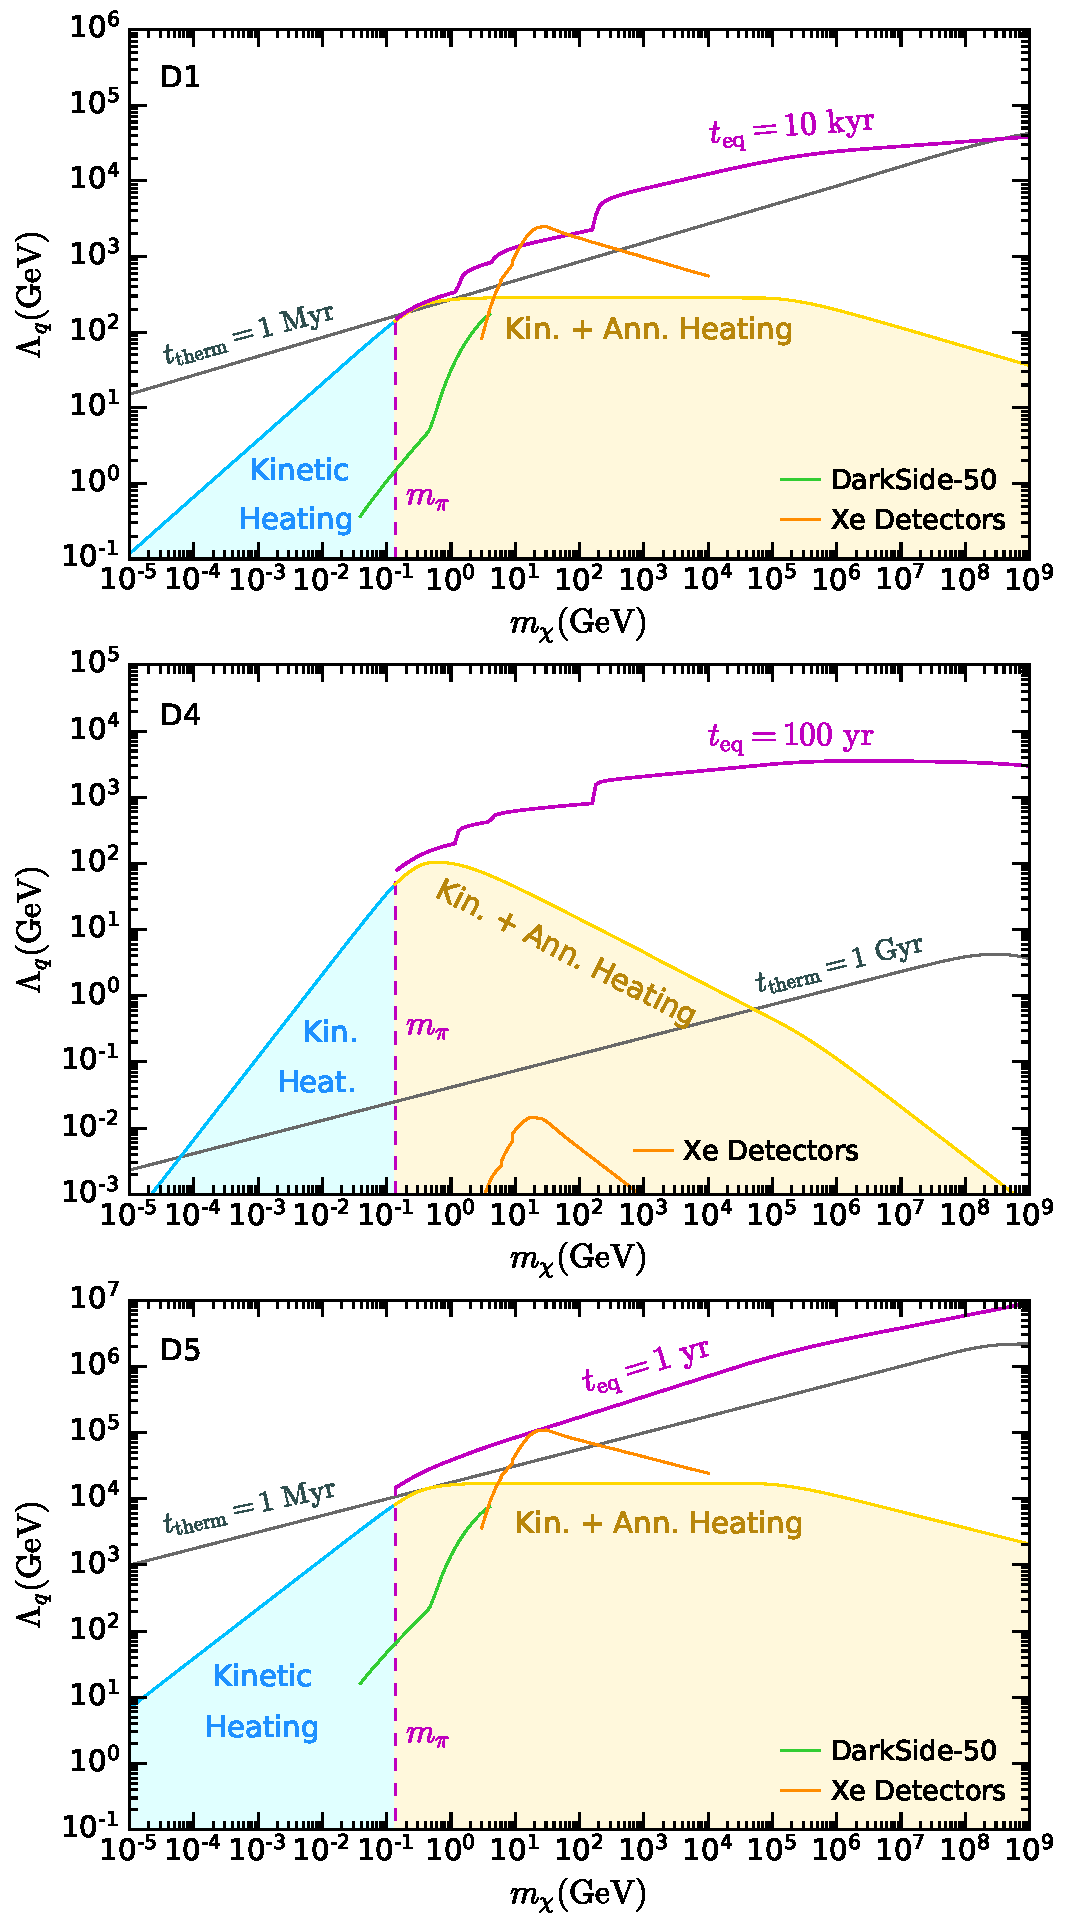
\includegraphics[width=0.6\textwidth]{ann_heat_sensitivity_3ops.pdf}   
    \caption{
    Projected NS heating sensitivity for maximal capture efficiency, for DM-baryon interactions described by operators D1, D4 and D5.  We have used the QMC-2 ($1.5\Msun$) benchmark NS configuration.
    We show the regions where DM kinetic and annihilation heating both contribute to the NS luminosity (yellow) and where kinetic heating alone contributes (light blue).
    Contour lines for capture-annihilation equilibrium (magenta) and thermalisation (grey) are shown for indicative timescales.    
     Lower limits on $\Lambda_q$ from leading  direct detection experiments~\cite{DarkSide:2022dhx_mar_SearchDarkMatterNucleon,XENON:2020gfr_mar_SearchCoherentElastic,PandaX-4T:2021bab_dec_DarkMatterSearch,LZ:2022lsv_jul_FirstDarkMatter} are also shown.  
    }
    \label{fig:NS_heating}
\end{figure}
%%%%%%%%%%%%%%%%%%%%%%%%%%%%%%%%%%%

We now examine the regions of parameter space where maximal heating can be achieved, for DM-hadron interactions described by the four-fermion operators of Table~\ref{tab:opers_defn_full}. As the extent of DM-induced heating depends on how efficiently the DM is captured, it is clear that maximal heating corresponds to the case of $f=1$ in Eqs.~\ref{eq:kinenergy} and~\ref{eq:massheating}, i.e., when the dark matter scattering cross-section is at or above the geometric limit. 


In Figure~\ref{fig:NS_heating}, we show the parameters for which the DM deposits its entire kinetic and rest mass energy (yellow region) or only its full kinetic energy (light blue region).  Above these shaded regions, the value of $\Lambda_q$ is too large (and hence the scattering cross-section is too small) for maximal capture.
The overall shape of the shaded regions is dictated by the behaviour of the capture rate. For sub-GeV DM, Pauli blocking suppresses the capture rate, and so smaller $\Lambda_q$ values are required to reach the geometric limit. At large DM mass, $\gtrsim 10^5\GeV$, the capture rate is suppressed because a single collision does not transfer enough energy to result in capture.


We see from the $\teq$ contours (magenta) that capture-annihilation equilibrium, and hence full annihilation heating, is achieved on a timescale much shorter that the NS lifetime, which we take to be $t_\star\sim 1\Gyr$. 
We do not show the contours for the kinetic heating timescale, $t_\mathrm{kin}$, as this is significantly shorter than the age of the star.  Moreover, for masses where DM annihilation to hadrons is possible, $m_\chi>m_\pi$, it is not necessary for kinetic heating to occur before capture-annihilation equilibrium is established, as the total kinetic plus mass energy will be deposited when the DM annihilates. 
For completeness, we include the contours of the thermalisation time (grey). We stress again that the DM does not need to fully thermalise to achieve maximal heating.


To highlight how the sensitivity varies for different interaction types, we show results for operators D1, D4 and D5 in Figure~\ref{fig:NS_heating}, with the remaining operators presented in Figure~\fixMV{fig:NSheating2}. These operators were chosen because they allow us to compare interactions with and without momentum or velocity-suppressed scattering or annihilation cross-sections. Specifically: 
\begin{itemize}
\item D1 (scalar): unsuppressed scattering cross-section; $p$-wave suppressed annihilation.
\item D4 (pseudoscalar): $q_{\rm tr}^4$ suppressed scattering cross-section; unsuppressed $s$-wave annihilation.
\item D5 (vector): unsuppressed scattering and annihilation cross-sections.
\end{itemize}

Comparing the projected NS heating sensitivity with limits from terrestrial direct detection experiments (shown as green and orange curves in Fig.~\ref{fig:NS_heating}) we find similar behaviour for D1 and D5. This is expected, as both of these operators give rise to unsuppressed spin-independent DM-nucleon scattering cross-sections. The $p$-wave suppression of the D1 annihilation cross-section increases $\teq$ compared to that for D5; nonetheless, equilibrium is reached relatively quickly compared to $t_\star$.  The D4 (pseudoscalar) interaction has dismal prospects of being observed in direct detection experiments, due to the severe  $q_{\rm tr}^4$ suppression for the scattering of non-relativistic DM. In contrast, NS heating has much greater sensitivity.

Note that the time required for complete thermalisation (grey contours) is much longer for D4 (momentum-suppressed scattering) than for D1 and D5. In fact, for operator D4, full thermalisation is not achieved for most of the interesting parameter space. This illustrates the importance of correctly identifying $\teq$ as the timescale on which full heating is achieved, rather than the much longer $\tth$. 



%%%%%%%%%%%%%%%%%%%%%%%%%%%%%%%%%%%%%%%%%%
\section{Interaction rate in the zero temperature approximation}
\label{sec:pauliblockingle}
%%%%%%%%%%%%%%%%%%%%%%%%%%%%%%%%%%%%%%%%%%



In this section,  we calculate the interaction rate in the zero temperature approximation for $\Msq = \alpha \, t^n$, where $n=0,1,2$ and $\alpha$ is a constant, in the low energy, Pauli suppressed regime where $K_\chi=E_\chi-m_\chi<\kinFi$. 
We assume the simplest scenario of constant target mass and point-like targets, as justified in Section~\ref{sec:thermstandard}. 

In this approximation, the interaction rate in the energy regime relevant for thermalization is given by~\cite{Bell:2020jou_sep_ImprovedTreatmentDark}
\begin{equation}
\Gamma^{-}(K_\chi,\Tstar=0) \propto \, \frac{1}{2^7\pi^3 K_\chi k }  \int_0^{K_\chi} q_0 dq_0 \,\, \int \frac{t_E^n dt_E }{\sqrt{q_0^2+t_E}}\Theta(\kinFi-q_0),
\label{eq:gammafinal}
\end{equation}
where $t_E=-t$,   and 
\begin{equation}
\int \frac{t_E^n dt_E }{\sqrt{q_0^2+t_E}} = 2D_n(q_0^2,t_E)\sqrt{q_0^2+t_E}.
\end{equation}
The $D_n$  functions can be found in Appendix B of  ref.~\cite{Bell:2020jou_sep_ImprovedTreatmentDark}. 
As we shall see, the integration intervals in Eq.~\ref{eq:gammafinal} depend on whether or not Pauli blocking suppresses any part of the thermalization process.
In both cases, we can find simple analytic approximations to these integrals. 
The minimal DM mass for which Pauli blocking is never in effect is denoted by $\mcrit$. 
  
We first consider the case where $m_\chi \lesssim \mcrit$. 
For the cases of $\mu \ll \kinFi/K_\chi$ or $\mu \gg K_\chi/\kinFi$, 
$\Gamma^{-}$ at first order in $K_\chi$ is given by
% 
\begin{align}
\Gamma^{-}(K_\chi) &\sim \frac{\alpha}{2^7\sqrt{2}\pi^3m_\chi^{3/2}K_\chi^{1/2}}\int_0^{K_\chi}q_0 dq_0 \left(\int_{t_{E}^{-}}^{t_{E}^{+}} \frac{t_E^n dt_E }{\sqrt{q_0^2+t_E}} \right)\\
&= \frac{\alpha}{2^6\sqrt{2}\pi^3m_\chi^{3/2}K_\chi^{1/2}}\int_0^{K_\chi}q_0 dq_0 \left(\sqrt{q_0^2+t_E^{+}}D_n(q_0^2,t_E^{+})-\sqrt{q_0^2+t_E^{-}}D_n(q_0^2,t_E^{-})\right), \label{eq:intratelowe}
\end{align}
% 
where $t_E^\pm$ are defined in ref.~\cite{Bell:2020jou_sep_ImprovedTreatmentDark}. 
For matrix elements independent of $t$ ($n=0$), we have $D_0(q_0^2,t_E^{\pm})=1$  and this result simplifies to
% 
\begin{align}
\Gamma_{n=0}^{-}(K_\chi) 
&\sim  \frac{|\overline{M}|^2}{2^6\pi^3m_\chi}\int_{0}^{K_\chi} dq_0 q_0 \left[\sqrt{2\left(1+\sqrt{1-\frac{q_0}{K_\chi}}\right)-\frac{q_0}{K_\chi}}-\sqrt{2\left(1-\sqrt{1-\frac{q_0}{K_\chi}}\right)-\frac{q_0}{K_\chi}}\right] \nonumber \\
&= \frac{|\overline{M}|^2}{120\pi^3m_\chi}K_\chi^2.
\end{align}
% 
We can rewrite the previous expression in terms of the DM-baryon scattering cross-section using the following expression
\begin{equation}
\sigma_{i\chi}^{n=0} = \frac{\Msq}{16\pi m_i^2 (1+\mu)^2}, 
\label{eq:intraten0}
\end{equation}
giving the interaction rate at first order in $K_\chi$
\begin{equation}
\Gamma_{n=0}^{-}(K_\chi)  \sim \frac{2 m_i}{15}\frac{(1+\mu)^2}{\mu}K_\chi^2 \sigma_{i\chi}^{n=0}.
\end{equation}
This result has the same $K_\chi$ and $\mu$ scaling as that of ref.~\cite{Bertoni:2013bsa_dec_DarkMatterThermalization}.



Performing a similar analysis for $\Msq=\alpha (-t)^n$, $n=1,2$, 
we find 
\begin{equation}
\Gamma_{n=1}^{-}(K_\chi) 
\sim \frac{2\alpha }{105\pi^3}K_\chi^3,\qquad 
\Gamma_{n=2}^{-}(K_\chi) 
\sim \frac{4\alpha }{63\pi^3}m_\chi K_\chi^4. 
\end{equation}
The expressions for the cross-sections for $n=1,2$ are 
\begin{equation}
\sigma^{n=1}_{i\chi} = \frac{\alpha}{16\pi m_i^2(1+\mu)^2}t_{max},\qquad
\sigma^{n=2}_{i\chi} = \frac{4}{3}\frac{\alpha}{16\pi m_i^2(1+\mu)^2}t_{max}^2.   
\end{equation}
These cross-sections must be normalized to sensible momentum transfer. We take this reference point to be the surface of the star, such that 
\begin{equation}
      t_{max} \sim \frac{4m_\chi^2}{1+\mu^2}\frac{1-B(\Rstar)}{B(\Rstar)}.   
\end{equation}
The interaction rates for $n=1,2$ can then be written as
\begin{eqnarray}
    \Gamma_{n=1}^{-}(K_\chi) &\sim& \frac{8}{105 \pi^2} \frac{(1+\mu)^2(1+\mu^2)}{\mu^2} \sigma_{\rm surf} \, K_\chi^3 \frac{B(\Rstar)}{1-B(\Rstar)}, \label{eq:intraten1}\\
\Gamma_{n=2}^{-}(K_\chi) &\sim& \frac{1}{21 \pi^2} \frac{(1+\mu)^2(1+\mu^2)^2}{\mu^3} \frac{\sigma_{\rm surf}}{m_i} \, K_\chi^4\left[\frac{B(\Rstar)}{1-B(\Rstar)}\right]^2.
\label{eq:intraten2}
\end{eqnarray}


We now look at the interaction rate in the super-heavy DM mass regime, $m_\chi \gtrsim \mcrit$.
The exact value of $\mcrit$ will depend on the NS configuration. However, we can take some typical values relevant to thermalization to give an estimate of its value. Taking $K_\chi=10^3\K$, $\kinFi=200\MeV$, we see that
\begin{equation}
    m_\chi \ge \frac{2\kinFi(2m_i+\kinFi)}{ K_\chi} \sim \frac{4\kinFi m_i}{K_\chi} = m_\chi^{\rm crit}\sim 9.65\times10^9\GeV. 
\end{equation}
The maximum energy transfer in this regime will always be $\qomax<K_\chi$, with
\begin{equation}
    \qomax\sim K_\chi\left[2\sqrt{\frac{m_\chi^{\rm crit}}{m_\chi }} - \frac{m_\chi^{\rm crit}}{m_\chi } +\mathcal{O}\left(\left(\frac{m_\chi^{\rm crit}}{m_\chi}\right)^{\frac{3}{2}}\right)\right].
 \end{equation}
Performing a similar analysis as the $m_\chi \lesssim \mcrit$ regime leads to the following expression for $\Gamma^-$,
\begin{equation}
\Gamma^{-}(K_\chi) \sim \frac{|\overline{M}|^2}{2^7\sqrt{2}\pi^3m_\chi^{3/2}K_\chi^{1/2}}\int_0^{	\qomax}q_0 dq_0 \left(\int_{t_{E}^{-}}^{t_{\mu^-}^{+}} \frac{t_E^n dt_E }{\sqrt{q_0^2+t_E}} \right),  
\end{equation} 
where $t_{\mu^-}^+$ is defined in ref.~\cite{Bell:2020jou_sep_ImprovedTreatmentDark}. 
For the simplest case of constant $|\overline{M}|^2$ this results in 
\begin{align}
\Gamma^{-}_{n=0}(K_\chi) & \sim  
\frac{K_\chi \kinFi |\overline{M}|^2}{24\pi^3\mu^2m_i}\left[\sqrt{\frac{m_\chi^{\rm crit}}{m_\chi}}+\mathcal{O}\left(\frac{m_\chi^{\rm crit}}{m_\chi}\right)\right] \nonumber\\
& = \frac{|\overline{M}|^2(m_i\kinFi)^{3/2}}{12 \pi^3m_\chi^{5/2}}K_\chi^{1/2}.\label{eq:intraten0largem}
\end{align}



%%%%%%%%%%%%%%%%%%%%%%%%%%%%%%%%%%%%%%%%%%%%%%%%%%%%%%%%%%%%%%%%%%%%%%%%%%%%%%%%%%%%
%%%%%%%%%%%%%%%%%%%%%%%%%%%%%%%%%%%%%%%%%%%%%%%%%%%%%%%%%%%%%%%%%%%%%%%%%%%%%%%%%%%%
\section{Thermalization of super-heavy DM}
\label{sec:thermsuperheavy}
%%%%%%%%%%%%%%%%%%%%%%%%%%%%%%%%%%%%%%%%%%%%%%%%%%%%%%%%%%%%%%%%%%%%%%%%%%%%%%%%%%%%
%%%%%%%%%%%%%%%%%%%%%%%%%%%%%%%%%%%%%%%%%%%%%%%%%%%%%%%%%%%%%%%%%%%%%%%%%%%%%%%%%%%%



For DM that is heavier than the critical mass  $m_\chi\gtrsim m_\chi^{\rm crit}$,
the energy lost in each scatter is a tiny fraction of the total DM kinetic energy. Moreover, the average time between collisions is typically on the order of fractions of a second. This warrants the use of a continuous approximation in this regime rather than performing the discrete summation. The thermalization time is then found by integrating the rate at which the DM kinetic energy changes, 
\begin{equation}
    \frac{dK_\chi}{dt} = -\Gamma^{-}(K_\chi) \langle\Delta K_\chi\rangle,  
    \label{eq:contttherm}
\end{equation}
from the initial kinetic energy, $K_\chi=m_\chi\left(\frac{1}{\sqrt{B(r)}}-1\right)$, to the final value $T_{\rm eq}\ll m_\chi$. For a constant cross-section ($n=0$), we substitute  Eqs.~\ref{eq:intraten0largem} and \ref{eq:aveElossn0largem} into the expression above leading to
\begin{equation}
    \tthn{0} \sim \frac{9 \pi^2 m_\chi}{8 (\mbeff)^2 \kinFi^2 \sigma_{i\chi}^{n=0}}\log\left[\frac{m_\chi}{T_{\rm eq}}\left(\frac{1}{\sqrt{B(\Rstar)}}-1\right)\right].
    \label{eq:tthemheavy0}
\end{equation}
Taking the final temperature to be $T_{\rm eq}=10^3\K$ and $B(\Rstar)=0.5$, this yields 
\begin{equation}
    \tthn{0} \sim 1.7  \yrs \left(\frac{m_\chi }{10^{10}\GeV}\right)\left(\frac{0.5\;m_n}{\mbeff(0)}\right)^{2}\left(\frac{0.2\GeV}{\kinFi(0)}\right)^{2}\left(\frac{10^{-45}\cm^2}{\sigma_{i\chi}^{n=0}}\right).    
\end{equation}
%
Repeating for $d\sigma\propto t^n$ ($n=1,2$), we calculate the thermalization time for $n=1$ to be
\begin{eqnarray}
    \tthn{1} &\sim& \frac{9\pi^2 m_\chi}{ 64 \mbeff \kinFi^3 \sigma_{i\chi}^{n=1}}\left[\frac{1-B(\Rstar)}{B(\Rstar)}\right] \log\left[\frac{m_\chi}{T_{\rm eq}} \left(\frac{1}{\sqrt{B(\Rstar)}}-1\right)\right],\\
    &\sim& 3.5 \yrs\; \left(\frac{m_\chi}{10^{10} \GeV}\right)\left(\frac{0.5\;m_n}{\mbeff(0)}\right) \left(\frac{0.2\GeV}{\kinFi(0)}\right)^{3}\left(\frac{10^{-45}\cm^2}{\sigma_{i\chi}^{n=1}}\right),
\end{eqnarray}
and that for $n=2$ to be
\begin{eqnarray}
    \tthn{2} &\sim& \frac{5 \pi^2 m_\chi}{ 32 \kinFi^4\sigma_{i\chi}^{n=2}} \left[\frac{1-B(\Rstar)}{B(\Rstar)}\right]^2 \log\left[\frac{m_\chi}{T_{\rm eq}}\left(\frac{1}{\sqrt{B(\Rstar)}}-1\right)\right],\\
    &\sim& 3.5 \yrs \left( \frac{m_\chi}{10^{10} \GeV}\right) \left(\frac{0.2\GeV}{\kinFi(0)}\right)^{4}\left(\frac{10^{-45}\cm^2}{\sigma_{i\chi}^{n=2}}\right). 
\end{eqnarray}







%%%%%%%%%%%%%%%%%%%%%%%%%%%%%%%%%%%%
\section{Thermalization time for $s$- and $t$-dependent interactions}
\label{sec:sdeptherm}
%%%%%%%%%%%%%%%%%%%%%%%%%%%%%%%%%%%%


In Section~\ref{sec:thermstandard}, we assumed $\Msq\propto t^n$ when deriving analytical approximations for the thermalization timescale. To understand the behavior of the thermalization time for the operators in Table.~\ref{tab:opers_defn_full}, we can make use of the results for $t^n$ dependent interactions. For cross-sections that are linear combinations of different powers of $t$, we can approximate the thermalization time using the previous results in the following way
\begin{align}
\Msq &= a_0 + a_1 t + a_2 t^2,\\
\sigma &= a_0\sigma_0 + a_1 \sigma_1 + a_2 \sigma_2,\\
\frac{1}{\tth} &\sim \frac{a_0}{ \tthn{0}(\sigma_{i\chi}=\sigma_0)} + \frac{a_1} {\tthn{1}(\sigma_{i\chi}=\sigma_1)} 
 + \frac{a_2}{  \tthn{2}(\sigma_{i\chi}=\sigma_2)}. 
\label{eq:ttherm_weighted}
\end{align}
Hence, the inverse of the thermalization time will be given by a weighted linear combination of the inverse times for each contribution. As higher powers of $t$ require significantly longer thermalization times, for coefficients of similar size, the resulting sum will be dominated by the lowest power of $t$ appearing in  $\Msq$.  We can thus identify the dominant terms for operators D1-D4  based on power counting, which we have listed in Table~\ref{tab:opers_defn_full}.

 For $s$-dependent amplitudes, we can in principle use the interaction rates calculated  in Appendix A of ref.~\cite{Bell:2020lmm_mar_ImprovedTreatmentDark}, perform a series expansion in $K_\chi$  and repeat the same procedure outlined in Section~\ref{sec:thermstandard} for $s$-independent matrix elements. Interestingly, we find that for the purpose of calculating the thermalization time, there is an easier way to obtain the correct result. One can indeed check that, at zero order in $\kinFi/\mbeff$, the resulting time for $s^1, s^2$ is equivalent to the constant case, with the matrix element calculated by setting 
\begin{equation}
    s\rightarrow (m_\chi+\mbeff)^2,
    \label{eq:ssubst}
\end{equation}
while the $s t $ case has a result equivalent to the $t$ case, with the matrix element calculated using the same substitution. This is, in practice, equivalent to setting both the DM and neutron targets at rest. There is, however, an important exception, when it comes to calculating the thermalization time of a linear combination of these terms. In particular, when the amplitudes at order $\mathcal{O}(t^0)$, are proportional to combinations of $1,s,s^2$ such as
\begin{gather}
s-(m_\chi+\mbeff)^2,\nonumber\\
\left[s-(m_\chi+\mbeff)^2\right]^2,\nonumber\\
\left[s-(\mbeff)^2-m_\chi^2\right]^2-4(\mbeff)^2 m_\chi^2.\label{eq:m2veldep}
\end{gather}
All these combinations give a null result after applying substitution \ref{eq:ssubst}. In such a case, one may think that the dominant term is given by some remaining $t^n$ term. It is worth noting that the expressions in  Eq.~\ref{eq:m2veldep}  appear in operators that, at low energy, are known as  velocity-dependent, because their matrix elements are proportional to positive even powers of the DM-target relative speed. Consequently, it is important not to neglect the motion of the targets in the neutron star, moving at relativistic speeds that are of the order of the Fermi velocity $v_F^2=2\kinFi/\mbeff$. In those cases, one should instead set $s$ to\footnote{We assume that $\mu\gg \mbeff/m_\chi^{\rm crit}$ when making this substitution.}
\begin{equation}
    s\rightarrow (m_\chi+\mbeff)^2+2m_\chi\kinFi.
    \label{eq:ssubstmu}
\end{equation}



In summary, operators D5, D8 and D9 can be safely expanded using \ref{eq:ssubst}, while operators D6, D7 and D10 have velocity-dependent amplitudes and require Eq.~\ref{eq:ssubstmu}. 
The dominant terms for each operator can be found in Table~\fixMV{Add the dominant terms in a new table}. 
For equal values of the leading term in $\Msq$, the thermalization time for each operator will be the same as the relevant $t^n$ power law. 


%%%%%%%%%%%%%%%%%%%%%%%%%%%%%%%%%%%%%%%%%%%%%%%%%%%%%%%%%%%%%%%
\section{Temperature distribution of captured dark matter}
\label{sec:minTempDerivation}
%%%%%%%%%%%%%%%%%%%%%%%%%%%%%%%%%%%%%%%%%%%%%%%%%%%%%%%%%%%%%%



As seen in Fig.~\ref{fig:thermtime}, interactions that depend on the momentum transfer, namely $d\sigma \propto t^n$ with $n = 1,2$, there are regions of the DM mass parameter space where thermalization does not occur within the age of the star. For the DM masses and NS temperatures of interest, this region of non-thermalization always occurs in the $m_\chi\ll \mcrit$ regime.
From Eqs.~\ref{eq:thermtimen0}, \ref{eq:thermtimen1} and \ref{eq:thermtimen2},  we can estimate the time required for the DM to reach a kinetic energy $K_\chi$ 
\begin{equation}
    t_{K_\chi} \propto \frac{1}{K_\chi^{n+2}}.
\end{equation}
% 
If the DM does not thermalize within the age of the star, it will instead reach a minimum temperature, $K_\chi^{\mathrm{min}}$.  Comparing the time required to achieve this temperature to the thermalization time, $\tth$ i.e. to have reached the equilibrium temperature $\Teq$, we find 
\begin{equation}
    \frac{t_{K_\chi^\mathrm{min}}}{\tth}  \sim \left( \frac{\Teq}{K^{\rm min}_\chi} \right)^{n+2}. 
\end{equation}
Accounting for the case where the DM reaches thermalization, we can write $K_\chi^\mathrm{min}$
\begin{align}
    K^{\rm min}_\chi & \sim \Teq \left(\max\left[ 1,\frac{\tth}{t_{K_\chi^\mathrm{min}}}\right ]\right)^{\frac{1}{n + 2}}\\
           & \approx \Teq \left( 1 + \frac{\tth}{t_{K_\chi^\mathrm{min}}}\right )^{\frac{1}{n + 2}}. 
\end{align}
The population of captured DM will have a distribution of energies at any given time, with this distribution being peaked at this minimum energy.
As the orbital periods of the DM will be much shorter than the average time between interactions, the DM will be able to virialize between each interaction. Therefore, we can treat the DM as being contained within an isothermal sphere with temperature $K^{\rm min}_\chi > \Teq$. 

Finally, it is worth noting that at times  $t>\tth$, even though the thermalization condition has been reached, the captured DM would consist of two components: a fraction of it (whose amount depends on time) would be in thermal equilibrium with the NS at temperature $T_{\rm eq}$; and another component still in the cooling down process. Assuming a  capture rate constant over time, the fraction of thermalized DM is 
\begin{equation}
    f_{\rm therm}(t) = \frac{t-t_{\rm therm}}{t}.
\end{equation}



%%%%%%%%%%%%%%%%%%%%%%%%%%%%%%%%%%%%%%%%%%%%%%%%%%%%%%%%%%%%%%%
\section{Quark-level vs hadron-level annihilation cross-sections}
\label{sec:quarkhadron}
%%%%%%%%%%%%%%%%%%%%%%%%%%%%%%%%%%%%%%%%%%%%%%%%%%%%%%%%%%%%%%%

The annihilation cross-sections shown in Table~\ref{tab:annCS} are for DM annihilation to quark final states.  More properly, we should consider the hadron-level annihilation cross-section.
However, we are primarily concerned with the capture-annihilation equilibrium timescale, and not the details of the annihilation process. Therefore, if the annihilation rate to hadrons is not significantly different from the quark level result, this subtlety can be avoided. 

To check the validity of the quark-level approximation, we estimate the annihilation rate to hadrons, working at lowest order in Chiral Perturbation Theory. We use couplings to the meson octet obtained from  ref.~\cite{Kumar:2018heq_dec_IndirectDetectionSubGeV}; for annihilation to baryons, the operators listed in Table~\ref{tab:opers_defn_full} are used. 
For DM masses in the range $m_\pi < m_\chi \lesssim m_{\rm charm} = 1.27\GeV$, we find that the cross-section for annihilation to hadrons differs by less than an order of magnitude than that for annihilation to quarks. For larger DM mass, the difference is negligible. Therefore, to simplify the discussion, we consider DM annihilation to quark final states for DM masses above the pion mass.


Below the pion mass, the only kinematically allowed DM annihilation channels would be to leptons or photons. The size of the DM couplings to these states would, in general, be unrelated to the DM-quark couplings we have assumed. (They are expected to be non-zero, because they would be induced at loop level~\cite{Bell:2019pyc_jun_CaptureLeptophilicDark}, even if absent at tree level.)
However, due to the considerable Fermi energies of the electrons and muons near the centre of the NS, these channels will be Pauli blocked for the whole DM mass range below $m_\pi$, forbidding these annihilations from occurring. To remain as model-independent as possible, we will not consider lepton and photon annihilation channels.

Figure~\ref{fig:ann_xs_plots} shows $t_{\rm eq}$ contour lines in the $\Lambda_q-m_\chi$ plane for the NS benchmark model QMC-2, $\Tstareq=1000\K$ and two representative operators D7 (left) and D8 (right). 
Operators whose thermally averaged annihilation cross-section $\sigmav$ has a  $m_f/m_\chi$ leading order term, namely D1-D4 and D8 (see Table~\ref{tab:annCS}), exhibit a sudden change in the slope wherever a new annihilation channel opens (see dotted lines on the right panel of Fig.~\ref{fig:ann_xs_plots}). Note that the higher the cutoff scale $\Lambda_q$, the lower the scattering and annihilation cross-sections, resulting in a larger $t_{\rm eq}$ timescale. For lower $\Teq$ temperatures, DM requires more time to reach both equilibrium conditions, thermalization and capture-annihilation. The variation of these results with respect to the NS configuration amounts at most to a factor of $\sim2$ in the $t_{\rm eq}$ contours (see shaded regions in the left panels) from the lightest configuration (QMC-1, $1\Msun$) to the heaviest (QMC-3, $1.9\Msun$) for most operators, with the sole exception of D4 for which this factor rises up to $\sim 2.4$. 

%%%%%%%%%%%%%%%%%%%%%%%%%%%%%%
\begin{figure*}
    \centering
    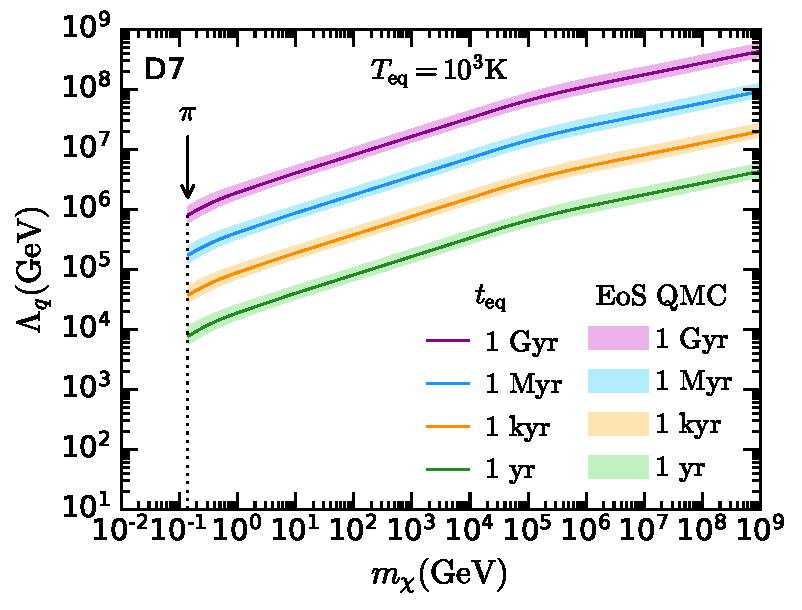
\includegraphics[width = 0.496\textwidth]{D7_Lambda_mdm_teq.pdf}
    \includegraphics[width = 0.496\textwidth]{D8_Lambda_mdm_teq.pdf}    
    \caption{
    Contours of the capture annihilation timescale, $t_{\rm eq}$,  in the $\Lambda_q-m_\chi$ plane for operators D7 (left) and D8 (right) and $\Tstareq=1000\K$. 
    Solid lines represent the calculation for the NS benchmark model QMC-2, and shaded regions denote the variation with the NS choice for the QMC EoS family. 
    Dotted lines in the right panel indicate the mass thresholds for various annihilation channels.  
    }
    \label{fig:ann_xs_plots}
\end{figure*}
%%%%%%%%%%%%%%%%%%%%%%%%%%%%%%%%%%%%%%


%%%%%%%%%%%%%%%%%%%%%%%%%%%%%%%%%%%%%%%%%%%%%%%%%%%%%%%%%%%%%%%
\section{Capture-annihilation equilibrium for the EFT operators}
\label{sec:resultsEFTop}
%%%%%%%%%%%%%%%%%%%%%%%%%%%%%%%%%%%%%%%%%%%%%%%%%%%%%%%%%%%%%%%

\begin{figure*}
    \centering
    \includegraphics[width=\textwidth]{ann_heat_sensitivity.pdf}    
    \caption{Projected NS heating sensitivity for maximal capture efficiency, for the full set of DM-baryon interactions described by the EFT operators of Table~\ref{tab:opers_defn_full}. We have used the QMC-2 ($1.5\Msun$) benchmark NS configuration.  
    Color coding as in Fig.~\ref{fig:NS_heating}. 
    }
    \label{fig:NS_heating2}
\end{figure*}



In Fig.~\ref{fig:NS_heating2}, we show isocontours of maximal capture (yellow and light blue lines) and capture-annihilation equilibrium (magenta lines) timescale in the $\Lambda_q-m_\chi$ plane for all  EFT operators.  
Values of $\Lambda_q$ below the $t_{\rm eq}$ lines result in smaller capture-annihilation equilibrium timescales. 
We can see in Fig.~\ref{fig:NS_heating} that for all operators the $t_{\rm eq}$ timescale is always smaller than the time required for captured DM to thermalize. Captured DM achieves the steady state condition in a timescale as short as $\sim1\yr$ (D1, D6-D10) or as long as $10^5\yr$ (D3). 
Note that the displayed lines for the $t_{\rm eq}$ are the values for which the entire parameter space relevant for capture reaches equilibrium with annihilation. 

For D1 and D6-D10, we observe that captured DM achieves thermal equilibrium in less than $\sim 1\Myr$ (grey lines). 
On the other hand, as expected from Fig.~\ref{fig:thermtime} captured DM whose interactions are momentum suppressed, namely operators D2-D4, would never thermalize to the temperature expected from DM-induced heating in $1\Gyr$, or even in less than the age of the 
Universe,
with the sole exception of the corner region of very light DM $m_\chi\lesssim 2\MeV$ and an even narrower corner of the parameter space for D4. 

Therefore, for all EFT operators,  the energy released in the annihilation process adds up to the energy deposited via capture increasing the DM-induced heating  
for $m_\chi\gtrsim m_\pi$ (yellow shaded area). 
Recall that we have made no assumptions about the energy scale that controls DM interactions with leptons. 
For DM of mass below $m_\pi$ (light blue lines), at least kinetic heating is expected to contribute to the star luminosity.  
\begin{comment}


\end{comment}
  

  \graphicspath{{img/chapter_6/}}

\chapter{Conclusion }
\label{chapter:conclusion}

\begin{synopsis}
  Concluding remarks
\end{synopsis}


  %% Glossary
  % \myglossaryentry{}{}{}{}
\myglossaryentry{NS}{NS}{Neutron Star}{}
\myglossaryentry{DM}{DM}{Dark Matter}{}
\myglossaryentry{QMC}{QMC}{Quark-Meson-Coupling EoS}{}
\myglossaryentry{EoS}{EoS}{Equation of State}{}
\myglossaryentry{$\bm t_{\rm eq}$}{tEq}{Capture-Annihilation equilibrium time}{}
\myglossaryentry{$\bm t_{\rm therm}$}{tTHerm}{Thermalisation time}{}
\myglossaryentry{$\bm m_\chi$}{DMmass}{Dark Matter Mass}{}
\myglossaryentry{$\bm C_{\rm geo}$}{Cgeo}{Geometric Capture Rate}{}
\myglossaryentry{EFT}{EFT}{Effective Field Theory}{}
\myglossaryentry{$\bm f_{\rm FD}$}{fermidirac}{Fermi-Dirac Distribution}{}
\myglossaryentry{$\bm T_{\rm eq}$}{Teq}{Equilibrium Temperature}{}
\myglossaryentry{$\bm T_\star$}{Tstar}{Temperature of the star}{}
\myglossaryentry{$\bm K_\chi$}{DMkinenergy}{Dark Matter Kinetic Energy}{}
\myglossaryentry{$\bm \mu$}{muDM}{DM-Target mass ratio, $m_\chi/m_i$}{}
\myglossaryentry{$\bm \varepsilon_{F, i}$}{fermiKin}{Fermi kinetic energy of target species}{}
\myglossaryentry{PB}{PB}{Pauli Blocking}{}
\myglossaryentry{$\bm \rho_\chi$}{DMlocaldens}{DM halo density}{}
\myglossaryentry{$\bm v_\star$}{vstar}{Star velocity}{}
\myglossaryentry{$\bm v_d$}{vdisp}{DM halo dispersion velocity}{}
\myglossaryentry{$\bm \sigmath$}{sigmath}{Threshold Cross Section}{}
\myglossaryentry{$\bm \Msq$}{Msqr}{Spin-averaged squared matrix element}{}


\end{mainmatter}

%%
%% Appendix
%%
\begin{appendices}
  \symmetricmargin

    %% Kinematics
    \graphicspath{{img/appendix_kinematics/}}
%%%%%%%%%%%%%%%%%%%%%%%%%%%%%%%%%%%%%%%%%%%%%%
\chapter{Kinematics}
\label{appendix:kinematics}
%%%%%%%%%%%%%%%%%%%%%%%%%%%%%%%%%%%%%%%%%%%%%%



\begin{synopsis}
  Kinematics
\end{synopsis}

%%%%%%%%%%%%%%%%%%%%%%%%%%%%%%%%%%%%%%%%%%%%%%
\section{DM Orbits in General Isometric Metric}
\label{sec:DM_orbits}
%%%%%%%%%%%%%%%%%%%%%%%%%%%%%%%%%%%%%%%%%%%%%%

As stated in section~\ref{sec:CO_general_structure}, the most general spherically symmetric, static metric is given by
\begin{equation}
    -ds^2 = B(r) dt^2 - A(r) dr^2 - r^2( d\theta + \sin\theta d\phi^2).
\end{equation}
We wish to study the properties of a particle moving along some orbit governed by this metric. 
Along an orbit, the conserved conjugate momenta are the angular momentum per unit mass, $p_\phi = -L$ 
and the energy per unit mass $p_t = E_\chi$, and taking the orbit to lie in the $\theta = \pi/2$ plane 
leads to $p_\theta = 0$. 

The equation which describes the orbit can be obtained from the square of the energy-momentum 4-vector,
\begin{align}
    g_{\alpha\beta} p^\alpha p^\beta - m_\chi^2 & = 0,\\
    \implies g^{\alpha\beta} p_\alpha p_\beta - m_\chi^2 & = 0,
\end{align}
with
\begin{equation}    
g^{tt} = 1/B(r),\quad g^{rr} = -1/A(r),\quad g^{\phi \phi} = -1/r^2.
\end{equation}

Changing from the 4-momenta $p^\mu$ to the conserved momenta, $p_\mu$ gives
\begin{align}
    0 & = g^{tt} p_t p_t + g^{rr} p_r p_r + g^{\phi\phi} p_\phi p_\phi - m_\chi^2 \\
    & = \frac{E_\chi^2}{B(r)} - \frac{1}{A(r)} \left( g_{rr'} p^{r'} \right)\left( g_{rr'} p^{r'} \right) - \frac{L^2}{r^2} - m_\chi^2 \\
    & = \frac{E_\chi^2}{B(r)} - m_\chi^2 A(r) \left( \frac{dr}{d\tau} \right)^2 - \frac{L^2}{r^2} - m_\chi^2.
\end{align}

To find $dt/d\tau$, we use
\begin{align}
    p^t & = m_\chi \frac{dt}{d\tau} = g^{tt}p_t = \frac{E_\chi}{B(r)}\\
    \implies \frac{dt}{d\tau} & = \frac{1}{B(r)}\frac{E_\chi}{m_\chi}.
\end{align}
% \Mcomm{In the papers we have $d\tau = \sqrt{B(r)} dt$, so where is the inconsistency?}

Finally, the orbit of the particle is described by the equation
\begin{equation}
    \left(\frac{dr}{dt} \right)^2 = \frac{B}{\tilde E_\chi^2 A} \left[\tilde E_\chi^2- B(r) \left(  1 + \frac{\tilde L^2}{r^2} \right) \right].
    \label{eq:drdt2GR}
\end{equation}

% \Mcomm{with alternative $dt/d\tau$
% \begin{equation}
%     \left (\frac{dr}{dt} \right)^2 = \frac{1}{A} \left[ \tilde E_\chi - B(r) \left( 1 + \frac{\tilde L^2}{r^2} \right) \right]
% \end{equation}
% }

For simplicity, we will consider orbits that are a straight line ($\tilde L = 0$), which has a radial extent $R$. This is related to $\tilde E_\chi$ through
\begin{gather}
    \tilde E_\chi^2 = B(R)\label{eq:maxradgeneral}\\
    \implies R = \frac{2 G M_\star}{1 - \tilde E_\chi^2}, \quad R>R_\star
    \label{eq:MaxRadius}
\end{gather}
using $B(r>R_\star) = 1 - 2 G M_\star /r$.

It is important to note that $E_\chi$ so far has been the \textit{conserved} energy along the orbit, 
which for the initial approach is $E_\chi = m_\chi + \frac{1}{2}m_\chi u^2\sim m_\chi$. 
We now call this energy $E_\chi^{\rm orbit}$, which is related to the DM energy as seen by a distant observer, $E_\chi^{\rm int}$, 
and is the energy used in calculating the interaction rates. These two quantities are related through 
\begin{equation}
    E_\chi^{\rm orbit} = \sqrt{g_{tt}} E_\chi^{\rm int} = \sqrt{B(r)}E_\chi^{\rm int},
\end{equation}
and as $E_\chi^{\rm orbit} < m_\chi$ for all subsequent scatters after capture, Eq.~\ref{eq:MaxRadius} is always positive.

These ``orbits" are straight lines that pass through the star's centre and extend an amount $R - R_\star$ on either side. 
Due to the symmetry of the motion, the period of the orbit is then
\begin{equation}
    T_{\rm orbit} = 4 \int_0^R \frac{1}{dr/dt}dr
\end{equation}
More relevant to this application is the time spent inside and outside the star, which is given by
\begin{align}
    T_{\rm inside} & = 4 \int_0^{R_\star} \frac{1}{dr/dt}dr\label{eq:timeinside}\\
    T_{\rm outside} & = 4 \int_{R_\star}^R \frac{1}{dr/dt}dr\label{eq:timeoutside}
\end{align}

% %%%%%%%%%%%%%%%%%%%%%%%%%%%%%%%%%%%%%%%%%%%%%%

% \section{Keeping Angular Dependence}
% %%%%%%%%%%%%%%%%%%%%%%%%%%%%%%%%%%%%%%%%%%%%%%

% For $\tilde L \neq 0$, we need the equation of motion for the angular coordinate $\phi$,

% \begin{align}
%     \frac{d \phi}{d\tau } & = g^{\phi\phi}p_\phi = \frac{\tilde L}{r^2}\\
%     \implies \frac{d\phi}{dt} & = \frac{B(r)}{\tilde E_\chi}\frac{\tilde L^2}{r^2}
% \end{align}
% The maximum value of  $\tilde L^2$ is  given by
% \begin{equation}
%     \tilde L^2_{\rm MAX} = \frac{ \tilde E_\chi^2 - B(r)}{B(r)}r^2
% \end{equation}
% and we parameterise the possible angular momentum along the orbit as 
% \begin{equation}
%     \tilde L^2 = y \tilde L^2_{\rm MAX} ,\quad 0<y<1.
% \end{equation}
% leading to the equation for $dr/dt$ simplifying to 
% \begin{equation}
%     \frac{dr}{dt} = \frac{B(r)}{\tilde E_\chi^2 A(r)}\left( \tilde E_\chi^2 - B(r) \right)(1 - y)
% \end{equation}
% showing that the maximum radius of the orbit does not change from the $\tilde L = 0$ case, only the time spent outside the star changes.

% % \begin{align}
% %     \frac{dt}{d\phi} & = \left( \frac{dt}{dr}\right)
% % \end{align}

% %%%%%%%%%%%%%%%%%%%%%%%%%%%%%%%%%%%%%%%%%%%%%%
% \section{Checking Newtonian/Non-Relativistic Limit}
% %%%%%%%%%%%%%%%%%%%%%%%%%%%%%%%%%%%%%%%%%%%%%%


% In the Newtonian limit, we take 
% \begin{align}
% B - 1\approx2 \phi \ll 1,\\
% A - 1 \approx - 2 G M(r) / r \equiv -2V(r)\ll 1,\\
% \tilde L^2 /r^2 \ll 1,\\
% \tilde E - 1 = \varepsilon \ll 1,
% \end{align}
% with $\varepsilon$ the non-relativistic energy per unit mass. Then expanding Eq.~\ref{eq:drdt2GR} we get
% \begin{align}
%     \left(\frac{dr}{dt}\right)^2 & = (1 + 2 \phi)(1 + 2V) - (1 + 2\phi)^2(1 + 2 V)(1 - 2 \varepsilon)\left(1 + \frac{\tilde L^2}{r^2}\right)\\
%     & = 1 + 2 \phi + 2 V - \left(1 + 4 \phi + 2 V + \frac{\tilde L^2}{r^2} - 2 \varepsilon \right)\\
%     & = -2 \phi - \frac{\tilde L^2}{r^2} + 2 \varepsilon\\
%     \implies \frac{1}{2}\left(\frac{dr}{dt}\right)^2 & +\frac{\tilde L^2}{ 2 r^2} + \phi = \varepsilon
% \end{align}
% which is the standard result for a Newtonian orbit.

    %%%%%%%%%%%%%%%%%%%%%%%%%%%%%%%%%%%%%%%%%%%%%%
%%%%%%%%%%%%%%%%%%%%%%%%%%%%%%%%%%%%%%%%%%%%%%
\chapter{Kinetic Heating}
\label{appendix:kin_heating}
%%%%%%%%%%%%%%%%%%%%%%%%%%%%%%%%%%%%%%%%%%%%%%
%%%%%%%%%%%%%%%%%%%%%%%%%%%%%%%%%%%%%%%%%%%%%%

%%%%%%%%%%%%%%%%%%%%%%%%%%%%%%%%%%%%%%%%%%%%%%
\section{DM Orbits in General Isometric Metric}
%%%%%%%%%%%%%%%%%%%%%%%%%%%%%%%%%%%%%%%%%%%%%%

The metric at any point inside or outside the NS can be written as 
\begin{equation}
    ds^2 = B(r) dt^2 - A(r) dr^2 - r^2( d\phi + \sin\theta d\theta^2)
\end{equation}
Along an orbit, the conserved conjugate momenta are the angular momentum per unit mass, $p_\phi = -L$ 
and the energy per unit mass $p_t = E_\chi$, and taking the orbit to lie in the $\theta = \pi/2$ plane 
leads to $p_\theta = 0$. 

The equation which describes the orbit can be obtained from the square of the energy-momentum 4-vector,
\begin{align}
    g_{\alpha\beta} p^\alpha p^\beta - m_\chi^2 & = 0\\
    \implies g^{\alpha\beta} p_\alpha p_\beta - m_\chi^2 & = 0
\end{align}
with
\begin{equation}    
g^{tt} = 1/B(r),\quad g^{rr} = -1/A(r),\quad g^{\phi \phi} = -1/r^2
\end{equation}
\begin{align}
    \implies 0 & = g^{tt} p_t p_t + g^{rr} p_r p_r + g^{\phi\phi} p_\phi p_\phi - m_\chi^2 \\
    & = \frac{E_\chi^2}{B(r)} - \frac{1}{A(r)} \left( g_{rr'} p^{r'} \right)\left( g_{rr'} p^{r'} \right) - \frac{L^2}{r^2} - m_\chi^2 \\
    & = \frac{E_\chi^2}{B(r)} - m_\chi^2 A(r) \left( \frac{dr}{d\tau} \right)^2 - \frac{L^2}{r^2} - m_\chi^2
\end{align}

To find $dt/d\tau$, we use
\begin{align}
    p^t & = m_\chi \frac{dt}{d\tau} = g^{tt}p_t = \frac{E_\chi}{B(r)}\\
    \implies \frac{dt}{d\tau} & = \frac{1}{B(r)}\frac{E_\chi}{m_\chi}
\end{align}
% \Mcomm{In the papers we have $d\tau = \sqrt{B(r)} dt$, so where is the inconsistency?}

This gives
\begin{equation}
    \left (\frac{dr}{dt} \right)^2 = \frac{B}{\tilde E_\chi^2 A} \left[\tilde E_\chi^2- B(r) \left(  1 + \frac{\tilde L^2}{r^2} \right) \right]\label{eq:drdt2GR}
\end{equation}

% \Mcomm{with alternative $dt/d\tau$
% \begin{equation}
%     \left (\frac{dr}{dt} \right)^2 = \frac{1}{A} \left[ \tilde E_\chi - B(r) \left( 1 + \frac{\tilde L^2}{r^2} \right) \right]
% \end{equation}
% }

For simplicity, consider orbits that are a straight line ($\tilde L = 0$), which has a radial extent $R$. This is related to $\tilde E_\chi$ through
\begin{gather}
    \tilde E_\chi^2 = B(R)\label{eq:maxradgeneral}\\
    \implies R = \frac{2 G M_\star}{1 - \tilde E_\chi^2}, \quad R>R_\star
    \label{eq:MaxRadius}
\end{gather}
using $B(r>R_\star) = 1 - 2 G M_\star /r$.

It is important to note that $E_\chi$ so far has been the \textit{conserved} energy along the orbit, 
which for the initial approach is $E_\chi = m_\chi + \frac{1}{2}m_\chi u^2\sim m_\chi$. 
We now call this energy $E_\chi^{\rm orbit}$, which is related to the DM energy as seen by a distant observer, $E_\chi^{\rm int}$, 
and is the energy used in calculating the interaction rates, through 
\begin{equation}
    E_\chi^{\rm orbit} = \sqrt{g_{tt}} E_\chi^{\rm int} = \sqrt{B(r)}E_\chi^{\rm int}
\end{equation}
and as $E_\chi^{\rm orbit} < m_\chi$ for all subsequent scatters after capture, eq.~\ref{eq:MaxRadius} is always positive.

These ``orbits" are straight lines that pass through the star's centre and extend an amount $R - R_\star$ on either side. 
Due to the symmetry of the motion, the period of the orbit is then
\begin{equation}
    T_{\rm orbit} = 4 \int_0^R \frac{1}{dr/dt}dr
\end{equation}
More relevant to this application is the time spent inside and outside the star, which is given by
\begin{align}
    T_{\rm inside} & = 4 \int_0^{R_\star} \frac{1}{dr/dt}dr\label{eq:timeinside}\\
    T_{\rm inside} & = 4 \int_{R_\star}^R \frac{1}{dr/dt}dr\label{eq:timeoutside}
\end{align}

% %%%%%%%%%%%%%%%%%%%%%%%%%%%%%%%%%%%%%%%%%%%%%%

% \section{Keeping Angular Dependence}
% %%%%%%%%%%%%%%%%%%%%%%%%%%%%%%%%%%%%%%%%%%%%%%

% For $\tilde L \neq 0$, we need the equation of motion for the angular coordinate $\phi$,

% \begin{align}
%     \frac{d \phi}{d\tau } & = g^{\phi\phi}p_\phi = \frac{\tilde L}{r^2}\\
%     \implies \frac{d\phi}{dt} & = \frac{B(r)}{\tilde E_\chi}\frac{\tilde L^2}{r^2}
% \end{align}
% The maximum value of  $\tilde L^2$ is  given by
% \begin{equation}
%     \tilde L^2_{\rm MAX} = \frac{ \tilde E_\chi^2 - B(r)}{B(r)}r^2
% \end{equation}
% and we parameterise the possible angular momentum along the orbit as 
% \begin{equation}
%     \tilde L^2 = y \tilde L^2_{\rm MAX} ,\quad 0<y<1.
% \end{equation}
% leading to the equation for $dr/dt$ simplifying to 
% \begin{equation}
%     \frac{dr}{dt} = \frac{B(r)}{\tilde E_\chi^2 A(r)}\left( \tilde E_\chi^2 - B(r) \right)(1 - y)
% \end{equation}
% showing that the maximum radius of the orbit does not change from the $\tilde L = 0$ case, only the time spent outside the star changes.

% % \begin{align}
% %     \frac{dt}{d\phi} & = \left( \frac{dt}{dr}\right)
% % \end{align}

%%%%%%%%%%%%%%%%%%%%%%%%%%%%%%%%%%%%%%%%%%%%%%
\section{Checking Newtonian/Non-Relativistic Limit}
%%%%%%%%%%%%%%%%%%%%%%%%%%%%%%%%%%%%%%%%%%%%%%


In the Newtonian limit, we take 
\begin{align}
B - 1\approx2 \phi \ll 1,\\
A - 1 \approx - 2 G M(r) / r \equiv -2V(r)\ll 1,\\
\tilde L^2 /r^2 \ll 1,\\
\tilde E - 1 = \varepsilon \ll 1,
\end{align}
with $\varepsilon$ the non-relativistic energy per unit mass. Then expanding Eq.~\ref{eq:drdt2GR} we get
\begin{align}
    \left(\frac{dr}{dt}\right)^2 & = (1 + 2 \phi)(1 + 2V) - (1 + 2\phi)^2(1 + 2 V)(1 - 2 \varepsilon)\left(1 + \frac{\tilde L^2}{r^2}\right)\\
    & = 1 + 2 \phi + 2 V - \left(1 + 4 \phi + 2 V + \frac{\tilde L^2}{r^2} - 2 \varepsilon \right)\\
    & = -2 \phi - \frac{\tilde L^2}{r^2} + 2 \varepsilon\\
    \implies \frac{1}{2}\left(\frac{dr}{dt}\right)^2 & +\frac{\tilde L^2}{ 2 r^2} + \phi = \varepsilon
\end{align}
which is the standard result for a Newtonian orbit.

\section{Procedure for calculating kinetic heating time}

\begin{itemize}
    \item Select a point in the star for the DM to scatter off, $r_{\rm scatter, 0}$. 
    \item DM comes in from infinity with initial energy $E_\chi \approx m_\chi$
    \item Boost DM to local energy of $m_\chi/\sqrt{B(r_{\rm scatter})}$
    \item Scatter the DM and calculate initial $\Delta E_\chi$
    \item Set local DM energy to $E_\chi \equiv p^t = m_\chi/\sqrt{B(r_{\rm scatter})} - \Delta E_\chi$
    \item Calculate the new conserved energy per unit mass along the orbit as 
    \begin{equation}
        \tilde E_\chi^{\rm orbit} = \sqrt{B(r_{\rm scatter})}E_\chi/m_\chi = \frac{\sqrt{B(r_{\rm scatter})}}{ m_\chi} (m_\chi/\sqrt{B(r_{\rm scatter, 0})} - \Delta E_\chi)
    \end{equation}
    \item Use Equation~\ref{eq:maxradgeneral} to solve for the maximum radius of the orbit, $R_{\rm orbit}$. 
    \item Use equations~\ref{eq:timeinside} and~\ref{eq:timeoutside} to calculate $T_{\rm in} / (T_{\rm in} + T_{\rm out})$
    \item Adjust the time interval between scatter by $dt\rightarrow dt (T_{\rm in} / (T_{\rm in} + T_{\rm out}))^{-1}$
    \item Iterate until $R_{\rm orbit} < R_\star$
\end{itemize}
\end{appendices}

%%
%% Back matter
%%
\glsaddall
\begin{backmatter}
    \symmetricmargin
    \frontmatterheadings
    \printglossary[style=mcolindex, title=Definition of Symbols and Abbreviations]
    \clearpage
    % \addcontentsline{toc}{chapter}{Index}
    % \printindex
    % \bibliographystyle{utphys}
    % \bibliography{src/refs_main}
    \printbibliography
\end{backmatter}

\end{document}
